% ==============================================================================
% Capítulo: Tracking Cinemático y Decodificación de la Dinámica Orofacial
% Proyecto: NANDU LSD - Sistema de Adquisición EMG y Cinemática Facial
% Institución: Laboratorio de Sistemas Dinámicos (LSD) - FCEyN, UBA
% ==============================================================================

\documentclass[11pt,a4paper]{report}
\usepackage[utf8]{inputenc}
\usepackage[spanish,es-nodecimaldot]{babel}
\usepackage{amsmath,amssymb,amsfonts}
\usepackage{graphicx}
\usepackage{booktabs}
\usepackage{geometry}
\usepackage{fancyhdr}
\usepackage{xcolor}
\usepackage{hyperref}
\usepackage{subcaption}

\geometry{top=2.5cm,bottom=2.5cm,left=2.5cm,right=2.5cm}

\pagestyle{fancy}
\fancyhf{}
\fancyhead[L]{\small\nouppercase{\leftmark}}
\fancyhead[R]{\small LSD - UBA}
\fancyfoot[C]{\thepage}

\definecolor{nandu_red}{HTML}{E63946}
\definecolor{nandu_blue}{HTML}{1F77B4}
\definecolor{nandu_green}{HTML}{2CA02C}
\definecolor{nandu_purple}{HTML}{9D4EDD}
\definecolor{nandu_amber}{HTML}{E7A61A}

\title{\textbf{Caracterización Cinemática Tridimensional y Decodificación Articulada del Habla mediante Visión Artificial}}
\author{Laboratorio de Sistemas Dinámicos (LSD) -- FCEyN, UBA}
\date{Noviembre 2026}

\begin{document}

\maketitle

\chapter{Cinemática Orofacial y Seguimiento Fiduciario 3D}

\section{Introducción y Marco Teórico}
El aparato fonador humano articula el habla mediante una coordinación espacio-temporal dinámica entre la musculatura profunda (intrínseca lingual, velopalatina y faríngea) y la musculatura facial superficial. Mientras que las señales mioeléctricas de superficie (sEMG) registran la activación neuromuscular de las unidades motoras superficiales, el seguimiento cinemático fiduciario permite medir directamente la deformación elástica externa del tejido facial y el desplazamiento mandibular.

En este capítulo se presenta el sistema de tracking cinemático tridimensional en tiempo real desarrollado para el proyecto Ñandú, evaluando su capacidad de decodificación y consistencia métrica frente a variaciones de cadencia fonatoria (24, 30 y 40 BPM), fluctuaciones de temporización (jitter anti-sincronización estocástico) e invarianza a perturbaciones de distancia y rotación cefálica.

\section{Diseño y Descripción de los Cuatro Bloques Experimentales}
Para aislar rigurosamente la dinámica motora orofacial y validar el comportamiento de las variedades latentes lineales y no lineales, se diseñaron y registraron cuatro bloques experimentales continuos bajo secuencias balanceadas de De Bruijn:
\begin{enumerate}
    \item \textbf{Bloque 1 -- Hiperarticulado (24 BPM, $\tau = 2.50\,\text{s}$):}
    Diseñado para caracterizar la máxima excursión fisiológica externa sin coarticulación opresiva. Cada vocal dispone de $2.5\,\text{s}$ para desplegar la fase preparatoria completa, meseta fonatoria y relajación elástica basal ($N=115$ pulsos limpios).
    \item \textbf{Bloque 2 -- Cadencia Natural con Jitter Estocástico (30 BPM, Jitter 15\%, $\tau \approx 1.75\,\text{s}$):}
    Simula la cadencia de habla cotidiana. Incorpora una modulación temporal pseudo-aleatoria (distribución de riesgo exponencial, $\pm 15\%$) entre pulsos consecutivos para romper la adaptación rítmica anticipatoria del sujeto ($N=115$ pulsos limpios).
    \item \textbf{Bloque 3 -- Cadencia Rápida con Coarticulación Severa (40 BPM, Jitter 20\%, $\tau \approx 1.80\,\text{s}$):}
    Régimen de alta velocidad fonatoria destinado a evaluar el límite biomecánico del aparato facial externo. Pone a prueba la hipótesis de hipo-articulación lingual compensatoria bajo coarticulación extrema ($N=135$ pulsos limpios).
    \item \textbf{Bloque 4 -- Invarianza de Distancia y Movimiento Cefálico (24 BPM):}
    Protocolo de estrés métrico y desacoplamiento espacial: dividido en tres fases continuas (posición estándar a $50\,\text{cm}$, retroceso intencional a $\approx 85\,\text{cm}$ reduciendo la escala óptica, y aproximación a $40\,\text{cm}$ con rotaciones cefálicas de cabeceo y guiñada de $\pm 10^\circ$). Evalúa la invarianza del algoritmo de Procrustes y la escala física milimétrica ($N=80$ pulsos limpios).
\end{enumerate}

\section{Metodología de Sensado y Geometría Fiduciaria}

\subsection{Adquisición Óptica y Calibración Fiduciaria}
La captura visual se realiza a través de un sensor RGB calibrado espacialmente. El marco fiduciario se construye a partir de una malla tridimensional densa (MediaPipe FaceMesh, 468 vértices métricos normalizados) estabilizada mediante filtrado adaptativo de doble escala (One-Euro Filter 3D) para suprimir el temblor de alta frecuencia sin introducir retardo de fase observable.

\begin{figure}[htbp]
    \centering
    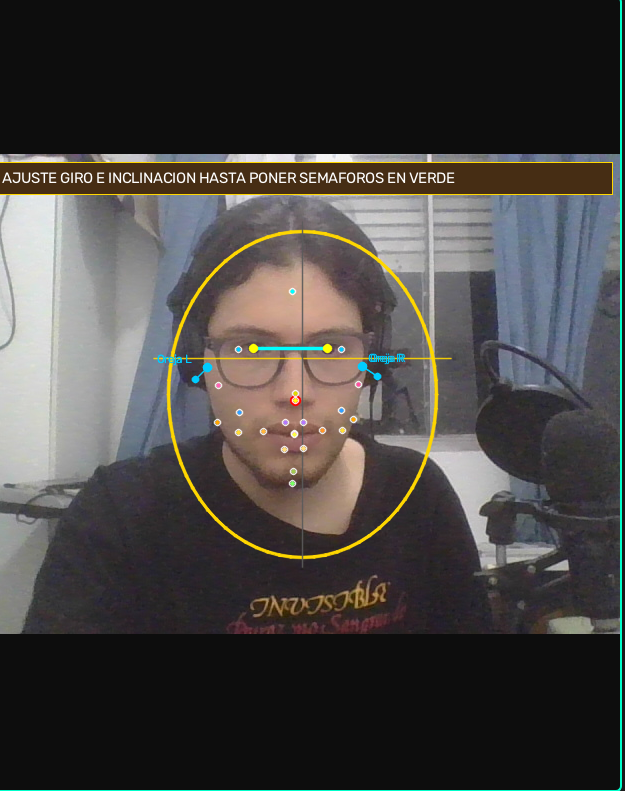
\includegraphics[width=0.48\textwidth]{figuras/foto_fiduciarios_calibracion.png}
    \caption{Asistente de calibración visual y orientación ortogonal en tiempo real. La elipse guía y los semáforos fiduciarios aseguran la alineación frontal, la distancia interocular basal y el centrado del plano cefálico antes del inicio de la secuencia continua.}
    \label{fig:calibracion_fiduciaria}
\end{figure}

\subsection{Cálculo de Variables Biomecánicas e Invarianza Rígida}
Para aislar la dinámica orofacial del movimiento global del torso y la cabeza, se implementa una transformación rígida tridimensional continua:
\begin{enumerate}
    \item \textbf{Alineación Ortogonal de Cráneo (Procrustes - Kabsch):} En cada cuadro de video $k$, se seleccionan puntos de anclaje óseo invariantes a la mímica (puente nasal $P_{\text{Sellion}}$, cantos oculares externos $P_{\text{Exo\_L}}, P_{\text{Exo\_R}}$ y procesos cigomáticos laterales). Se resuelve la matriz de rotación óptima $R_k \in \mathrm{SO}(3)$ y traslación $t_k \in \mathbb{R}^3$ respecto a la pose neutral de reposo:
    \begin{equation}
        \min_{R_k, t_k} \sum_{i \in \text{fijos}} \| P_i^{(0)} - (R_k P_i^{(k)} + t_k) \|^2
    \end{equation}
    \item \textbf{Calibración a Escala Física Real (mm):} La escala métrica $s_{\text{mm/px}}$ se calibra dinámicamente utilizando la distancia interocular fiduciaria fotorreflectiva ($D_{\text{ojo}} = 63.0\,\text{mm}$ basal):
    \begin{equation}
        s_{\text{mm/px}} = \frac{D_{\text{ojo, mm}}}{\| P_{\text{pupila\_L}} - P_{\text{pupila\_R}} \|_{\text{px}}}
    \end{equation}
    \item \textbf{Derivación de Variables Cinemáticas de 3 y 6 Canales:}
    A partir de los puntos fiduciarios proyectados en el marco corregido, se extraen las siguientes series temporales:
    \begin{itemize}
        \item \textbf{Apertura Mandibular ($c_1$):} Desplazamiento interlabial vertical y descenso del mentón (Gnathion fiduciario respecto al plano subnasal):
        \begin{equation}
            c_1(t) = (y_{\text{labio\_inf}}(t) - y_{\text{labio\_sup}}(t)) \cdot s_{\text{mm/px}} - \text{baseline}_{\text{ap}}
        \end{equation}
        \item \textbf{Ancho de Comisuras ($c_2$):} Distancia horizontal intercomisural (Cheilion izquierdo a Cheilion derecho):
        \begin{equation}
            c_2(t) = \max\left(0, \| P_{\text{comisura\_der}}(t) - P_{\text{comisura\_izq}}(t) \| \cdot s_{\text{mm/px}} - \text{baseline}_{\text{com}}\right)
        \end{equation}
        \item \textbf{Constricción Esfinteriana ($c_3$):} Reducción horizontal de comisuras y protrusión:
        \begin{equation}
            c_3(t) = \max\left(0, \text{baseline}_{\text{com}} - \| P_{\text{comisura\_der}}(t) - P_{\text{comisura\_izq}}(t) \| \cdot s_{\text{mm/px}}\right)
        \end{equation}
        \item \textbf{Variables Bio-Inspiradas Expandidas ($c_4, c_5, c_6$):} Distancias locales de retracción bucal (comisura a buccinador), elevación malar (comisura a arco cigomático menor) y compresión maseterina (comisura a gonion/masetero).
    \end{itemize}
\end{enumerate}

\subsection{Sincronización Multimodal y Parámetros de Filtrado Canónicos}
Conforme a la convención canónica del laboratorio, se adoptan los siguientes parámetros de acondicionamiento de señal:
\begin{itemize}
    \item \textbf{Master Clock Acústico:} Envolvente RMS calculada sobre el audio a $44.1\,\text{kHz}$ con ventana canónica inviolable de $250\,\text{ms}$. El instante $t=0$ se ancla dinámicamente al pico de intensidad fónica en cada pulso.
    \item \textbf{Suavizado Cinemático:} Filtro uniforme pasabajos continuo con ventana de $125\,\text{ms}$ adaptada a los cuadros por segundo efectivos de la cámara ($\text{FPS} \approx 29.5\,\text{Hz}$).
    \item \textbf{Ventana de Recorte Dinámica ($40\% - 60\%$):} En cada experimento con cadencia de pulso de período $\tau = \frac{60}{\text{BPM}}$, la ventana fónica se recorta asimétricamente respetando:
    \begin{equation}
        t_{\text{inicio}} = -0.40 \cdot \tau, \qquad t_{\text{fin}} = +0.60 \cdot \tau
    \end{equation}
    \item \textbf{Purga de Artefactos:} Aislamiento multivariado no lineal mediante \textit{Isolation Forest} con 8\% de contaminación máxima por clase.
\end{itemize}

\newpage
\section{Patrones Cinemáticos de Activación (3 Canales Directos)}
A continuación se presentan las curvas temporales promedio sincronizadas en $t=0$ para los 4 bloques experimentales. Todas las filas comparten escala vertical fija para garantizar comparabilidad directa de amplitudes.

\begin{figure}[htbp]
    \centering
    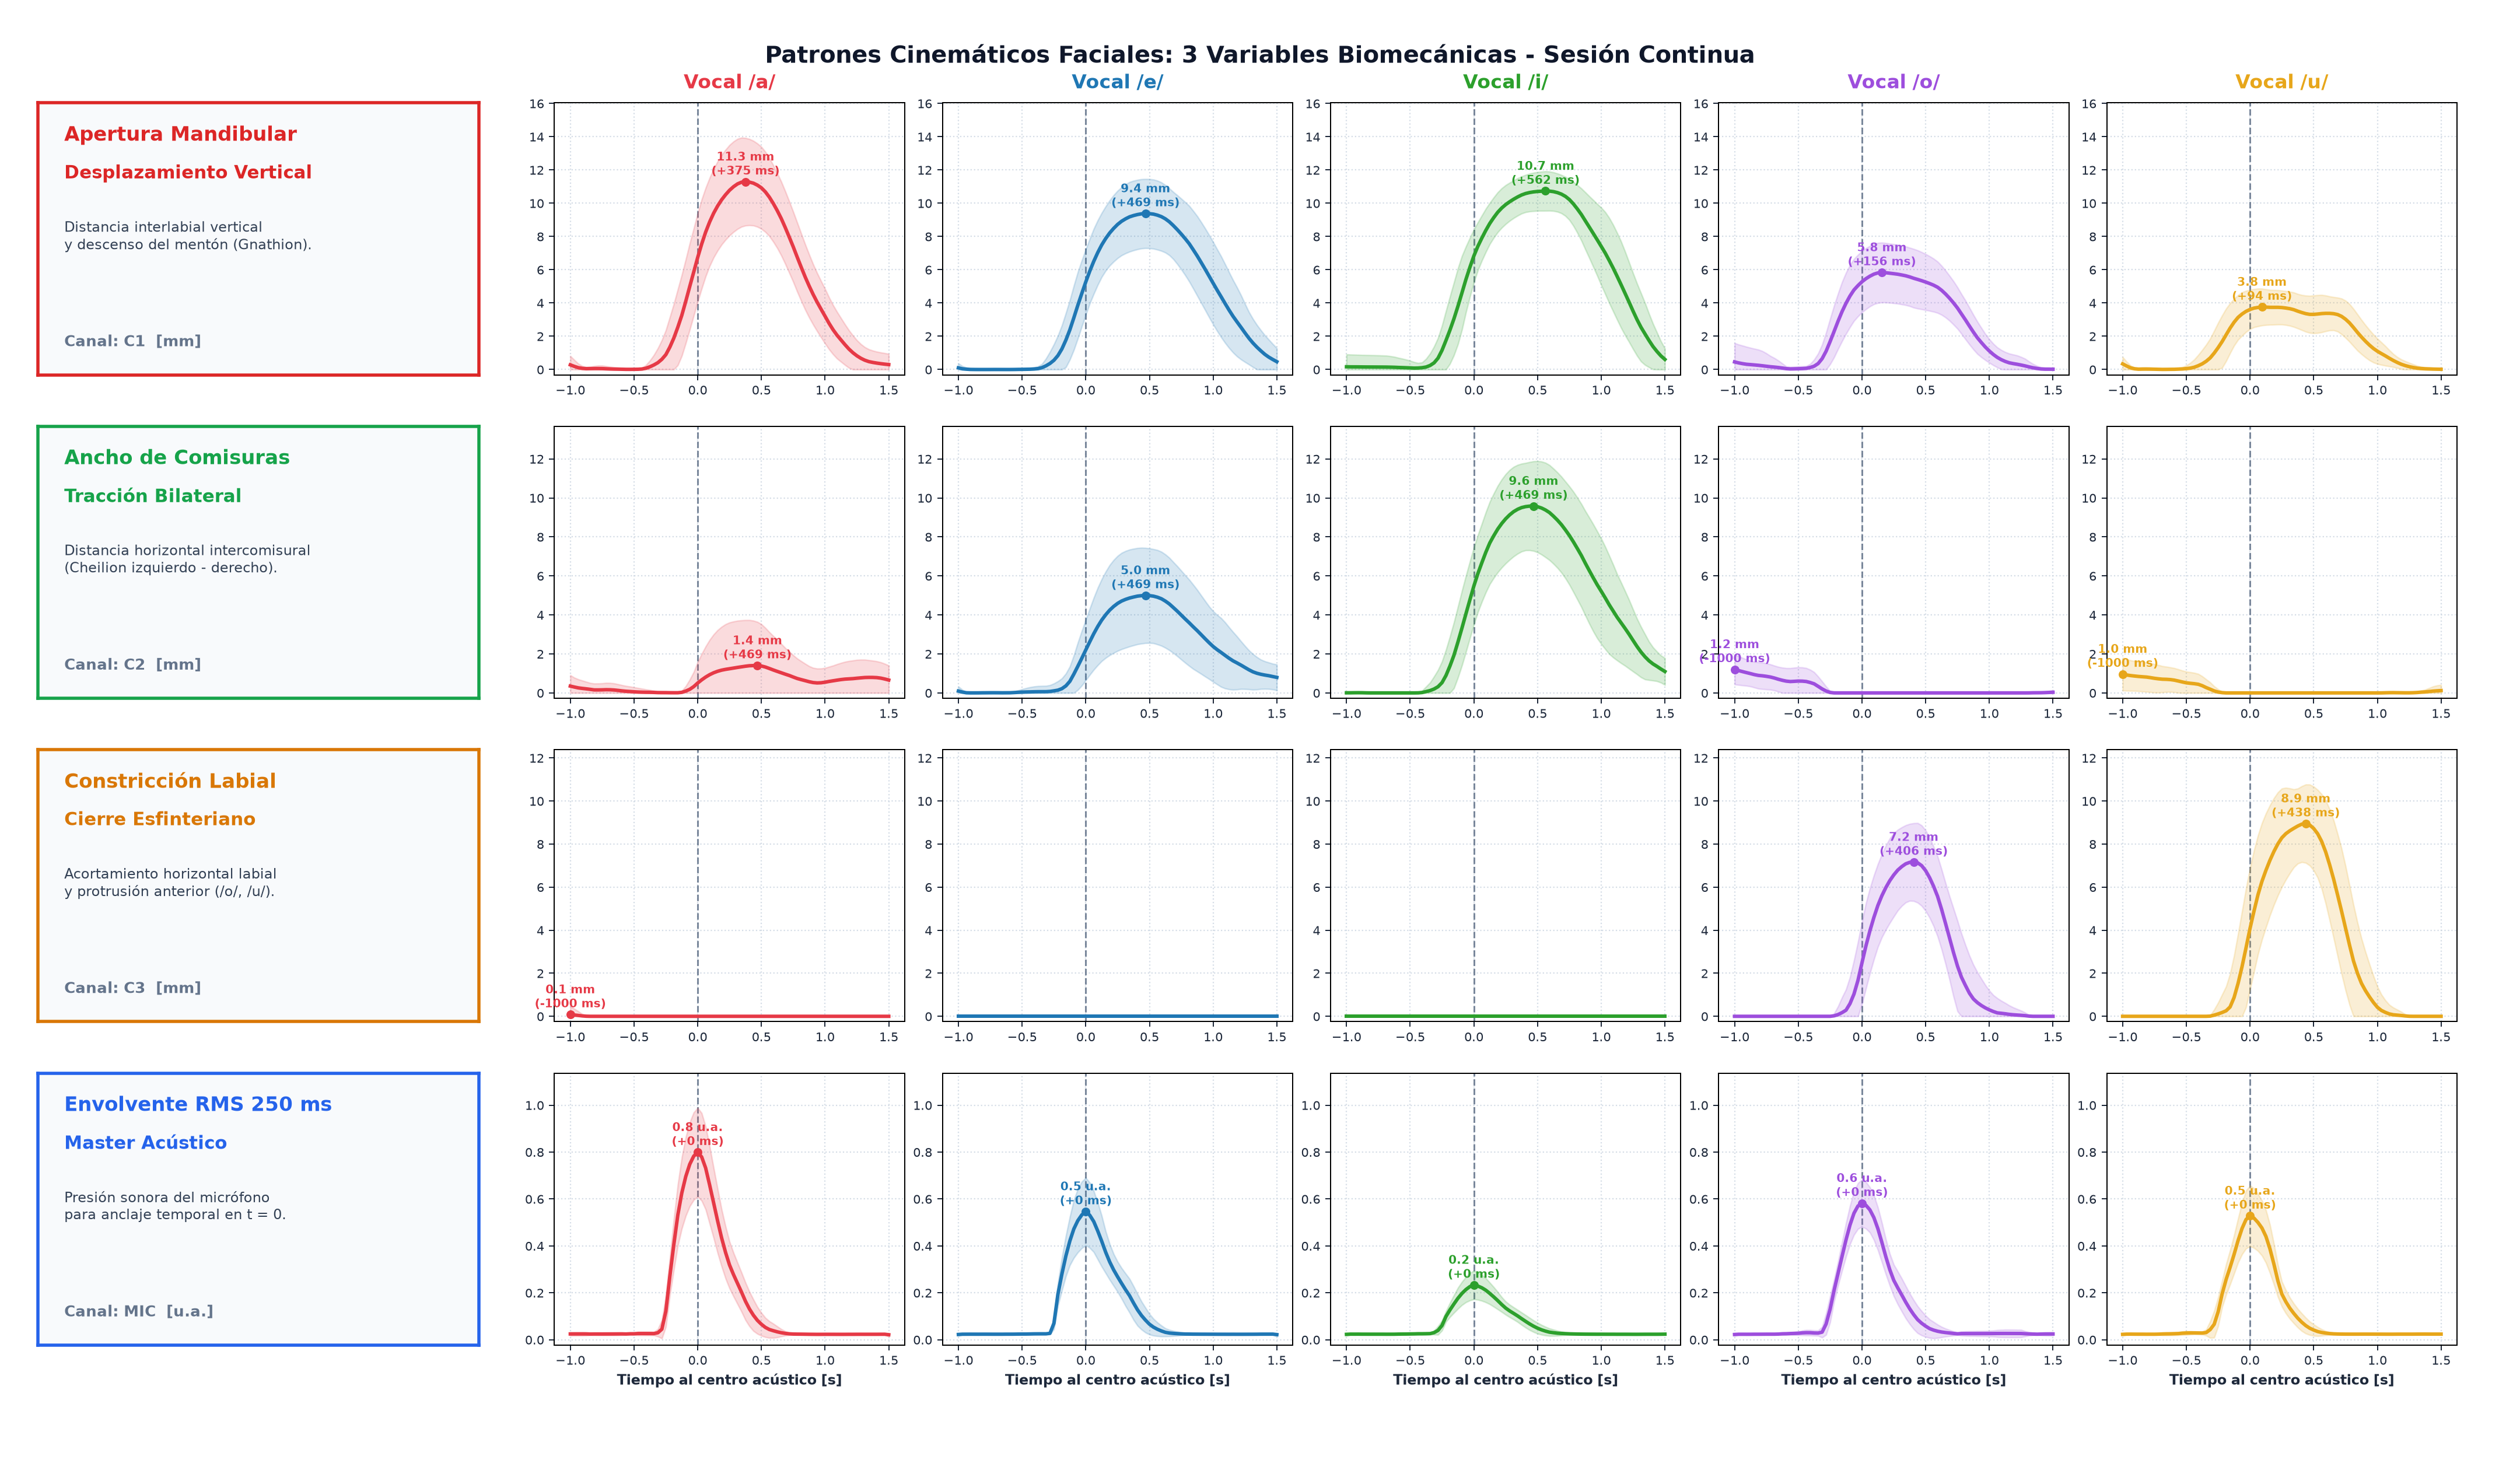
\includegraphics[width=0.98\textwidth]{figuras/exp1/patrones_cineticos_oficial.png}
    \caption{Patrones cinemáticos de 3 canales -- Experimento 1: Hiperarticulado 24 BPM (Secuencia De Bruijn balanceada, $\tau = 2.50\,\text{s}$).}
    \label{fig:pat_3ch_exp1}
\end{figure}

\begin{figure}[htbp]
    \centering
    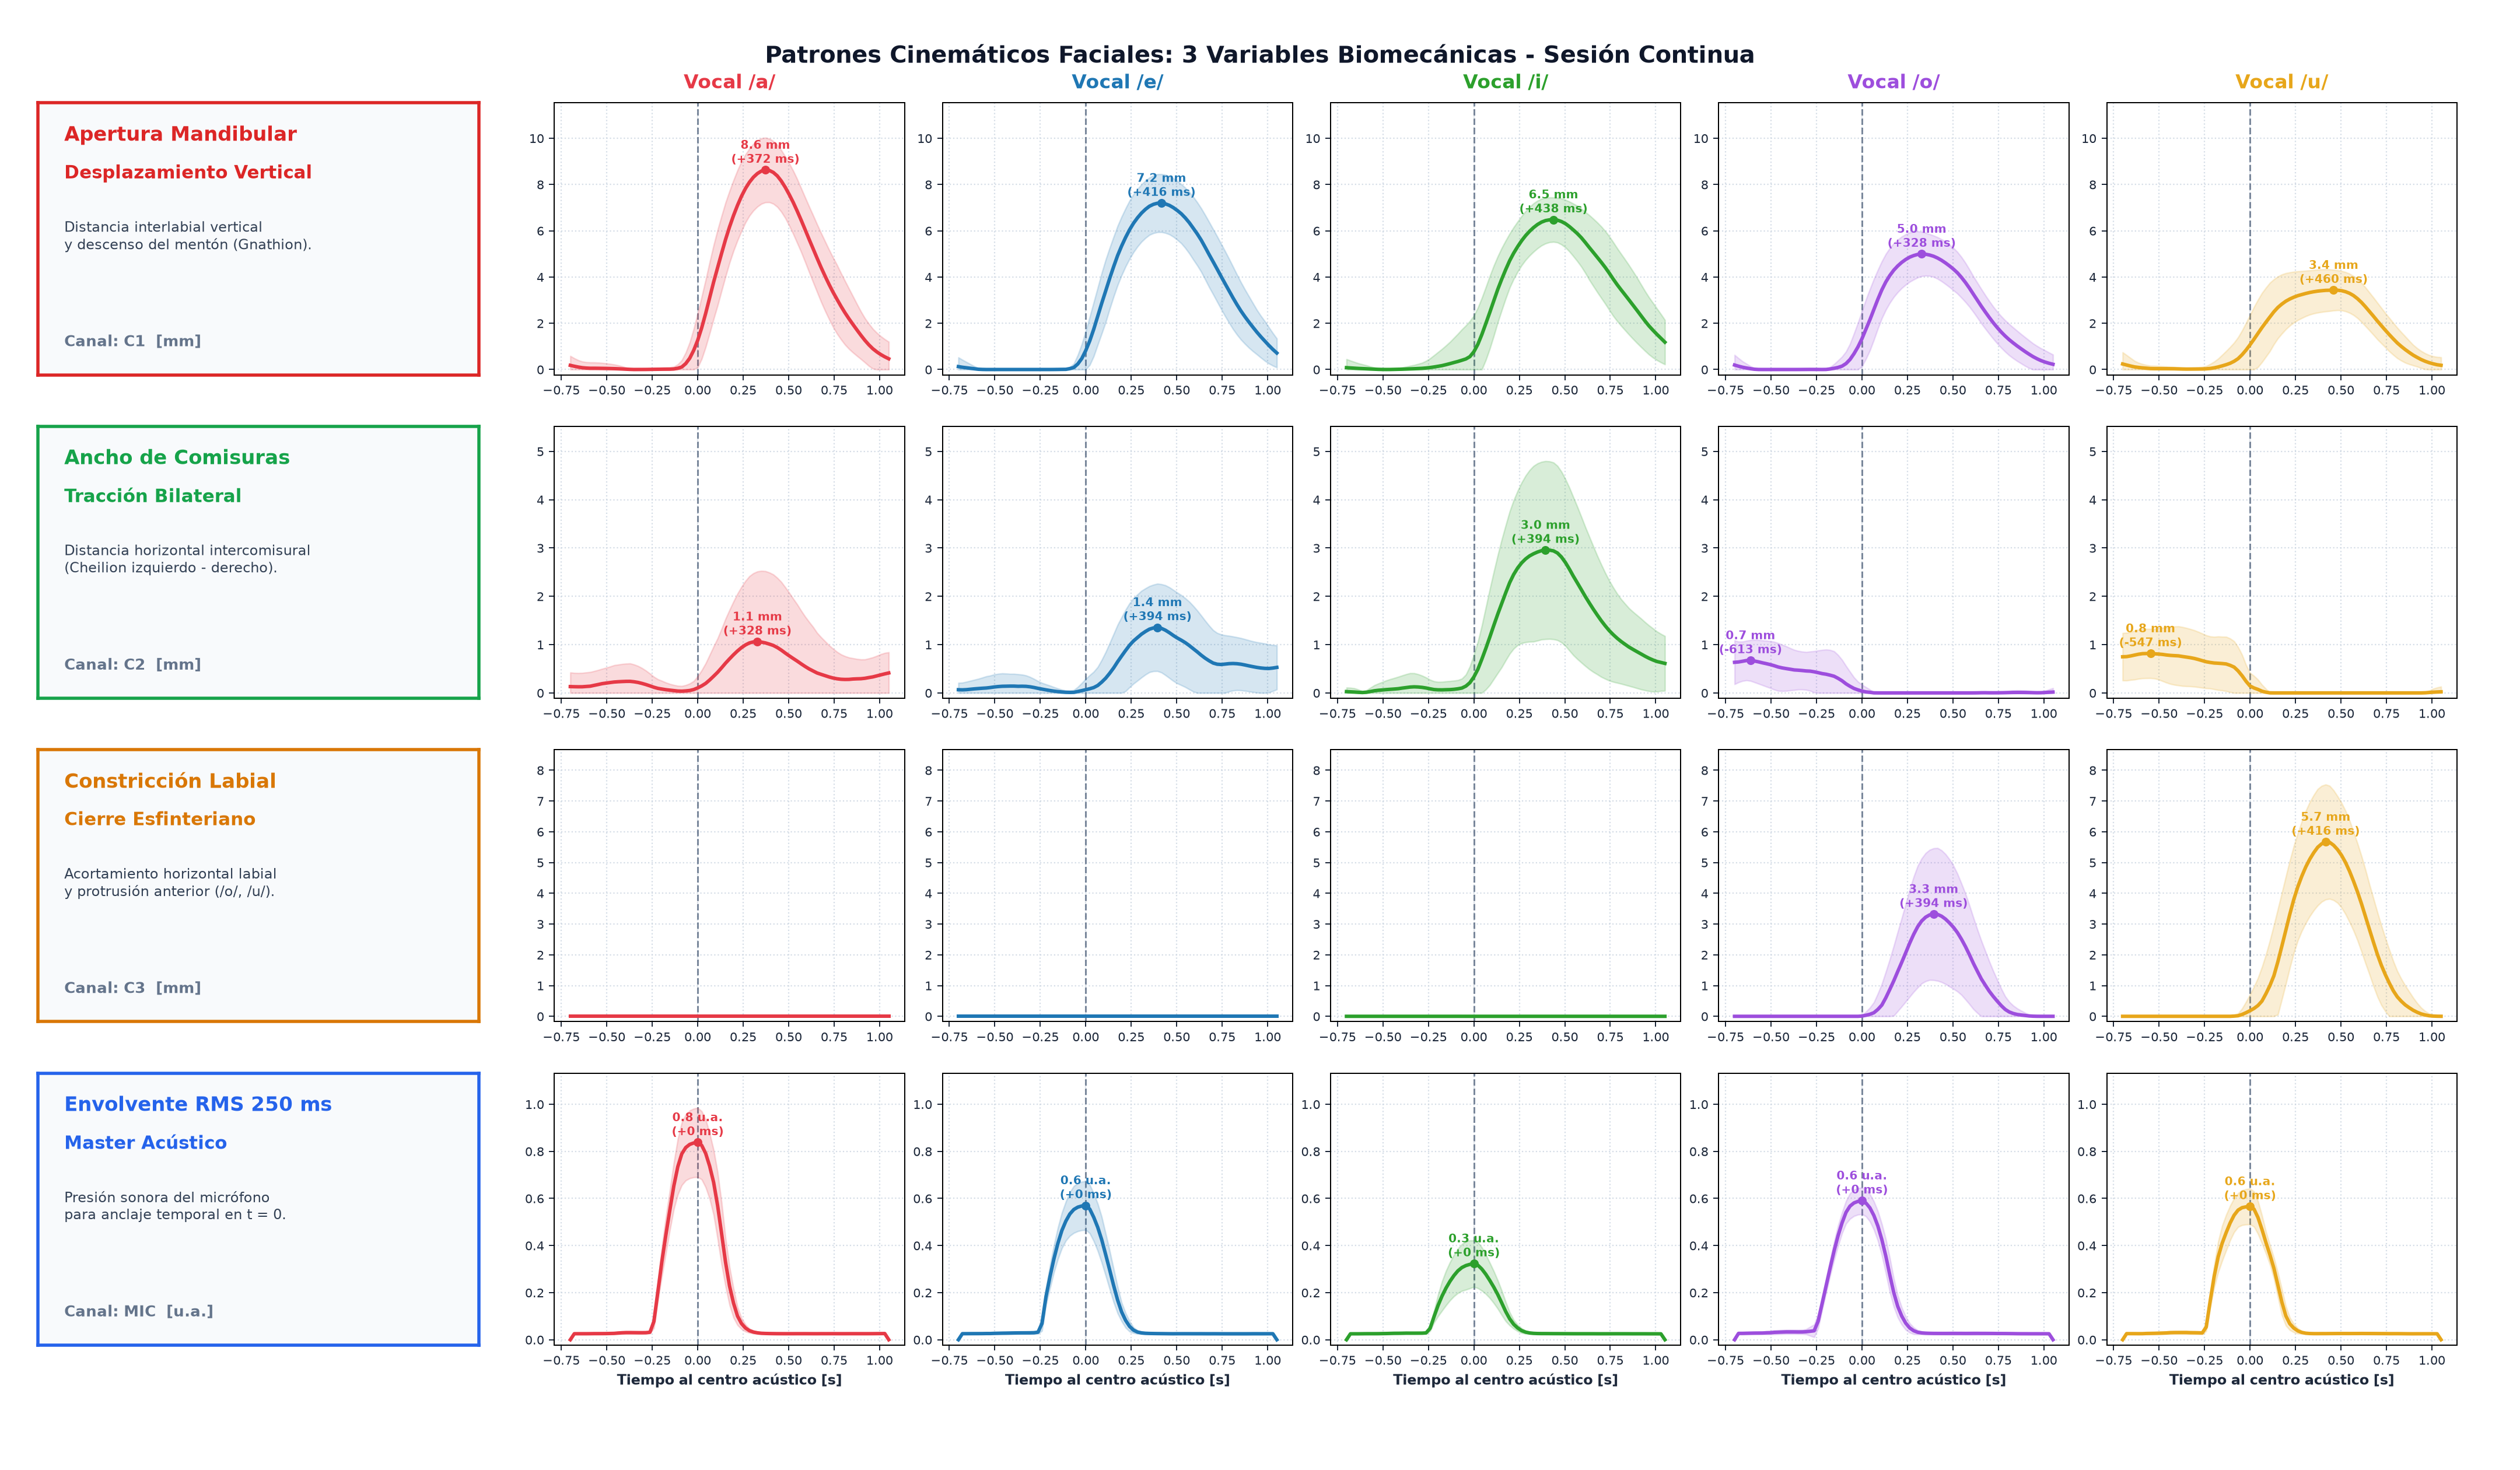
\includegraphics[width=0.98\textwidth]{figuras/exp2/patrones_cineticos_oficial.png}
    \caption{Patrones cinemáticos de 3 canales -- Experimento 2: Cadencia Natural 30 BPM con Jitter estocástico del 15\% ($\tau \approx 1.75\,\text{s}$).}
    \label{fig:pat_3ch_exp2}
\end{figure}

\begin{figure}[htbp]
    \centering
    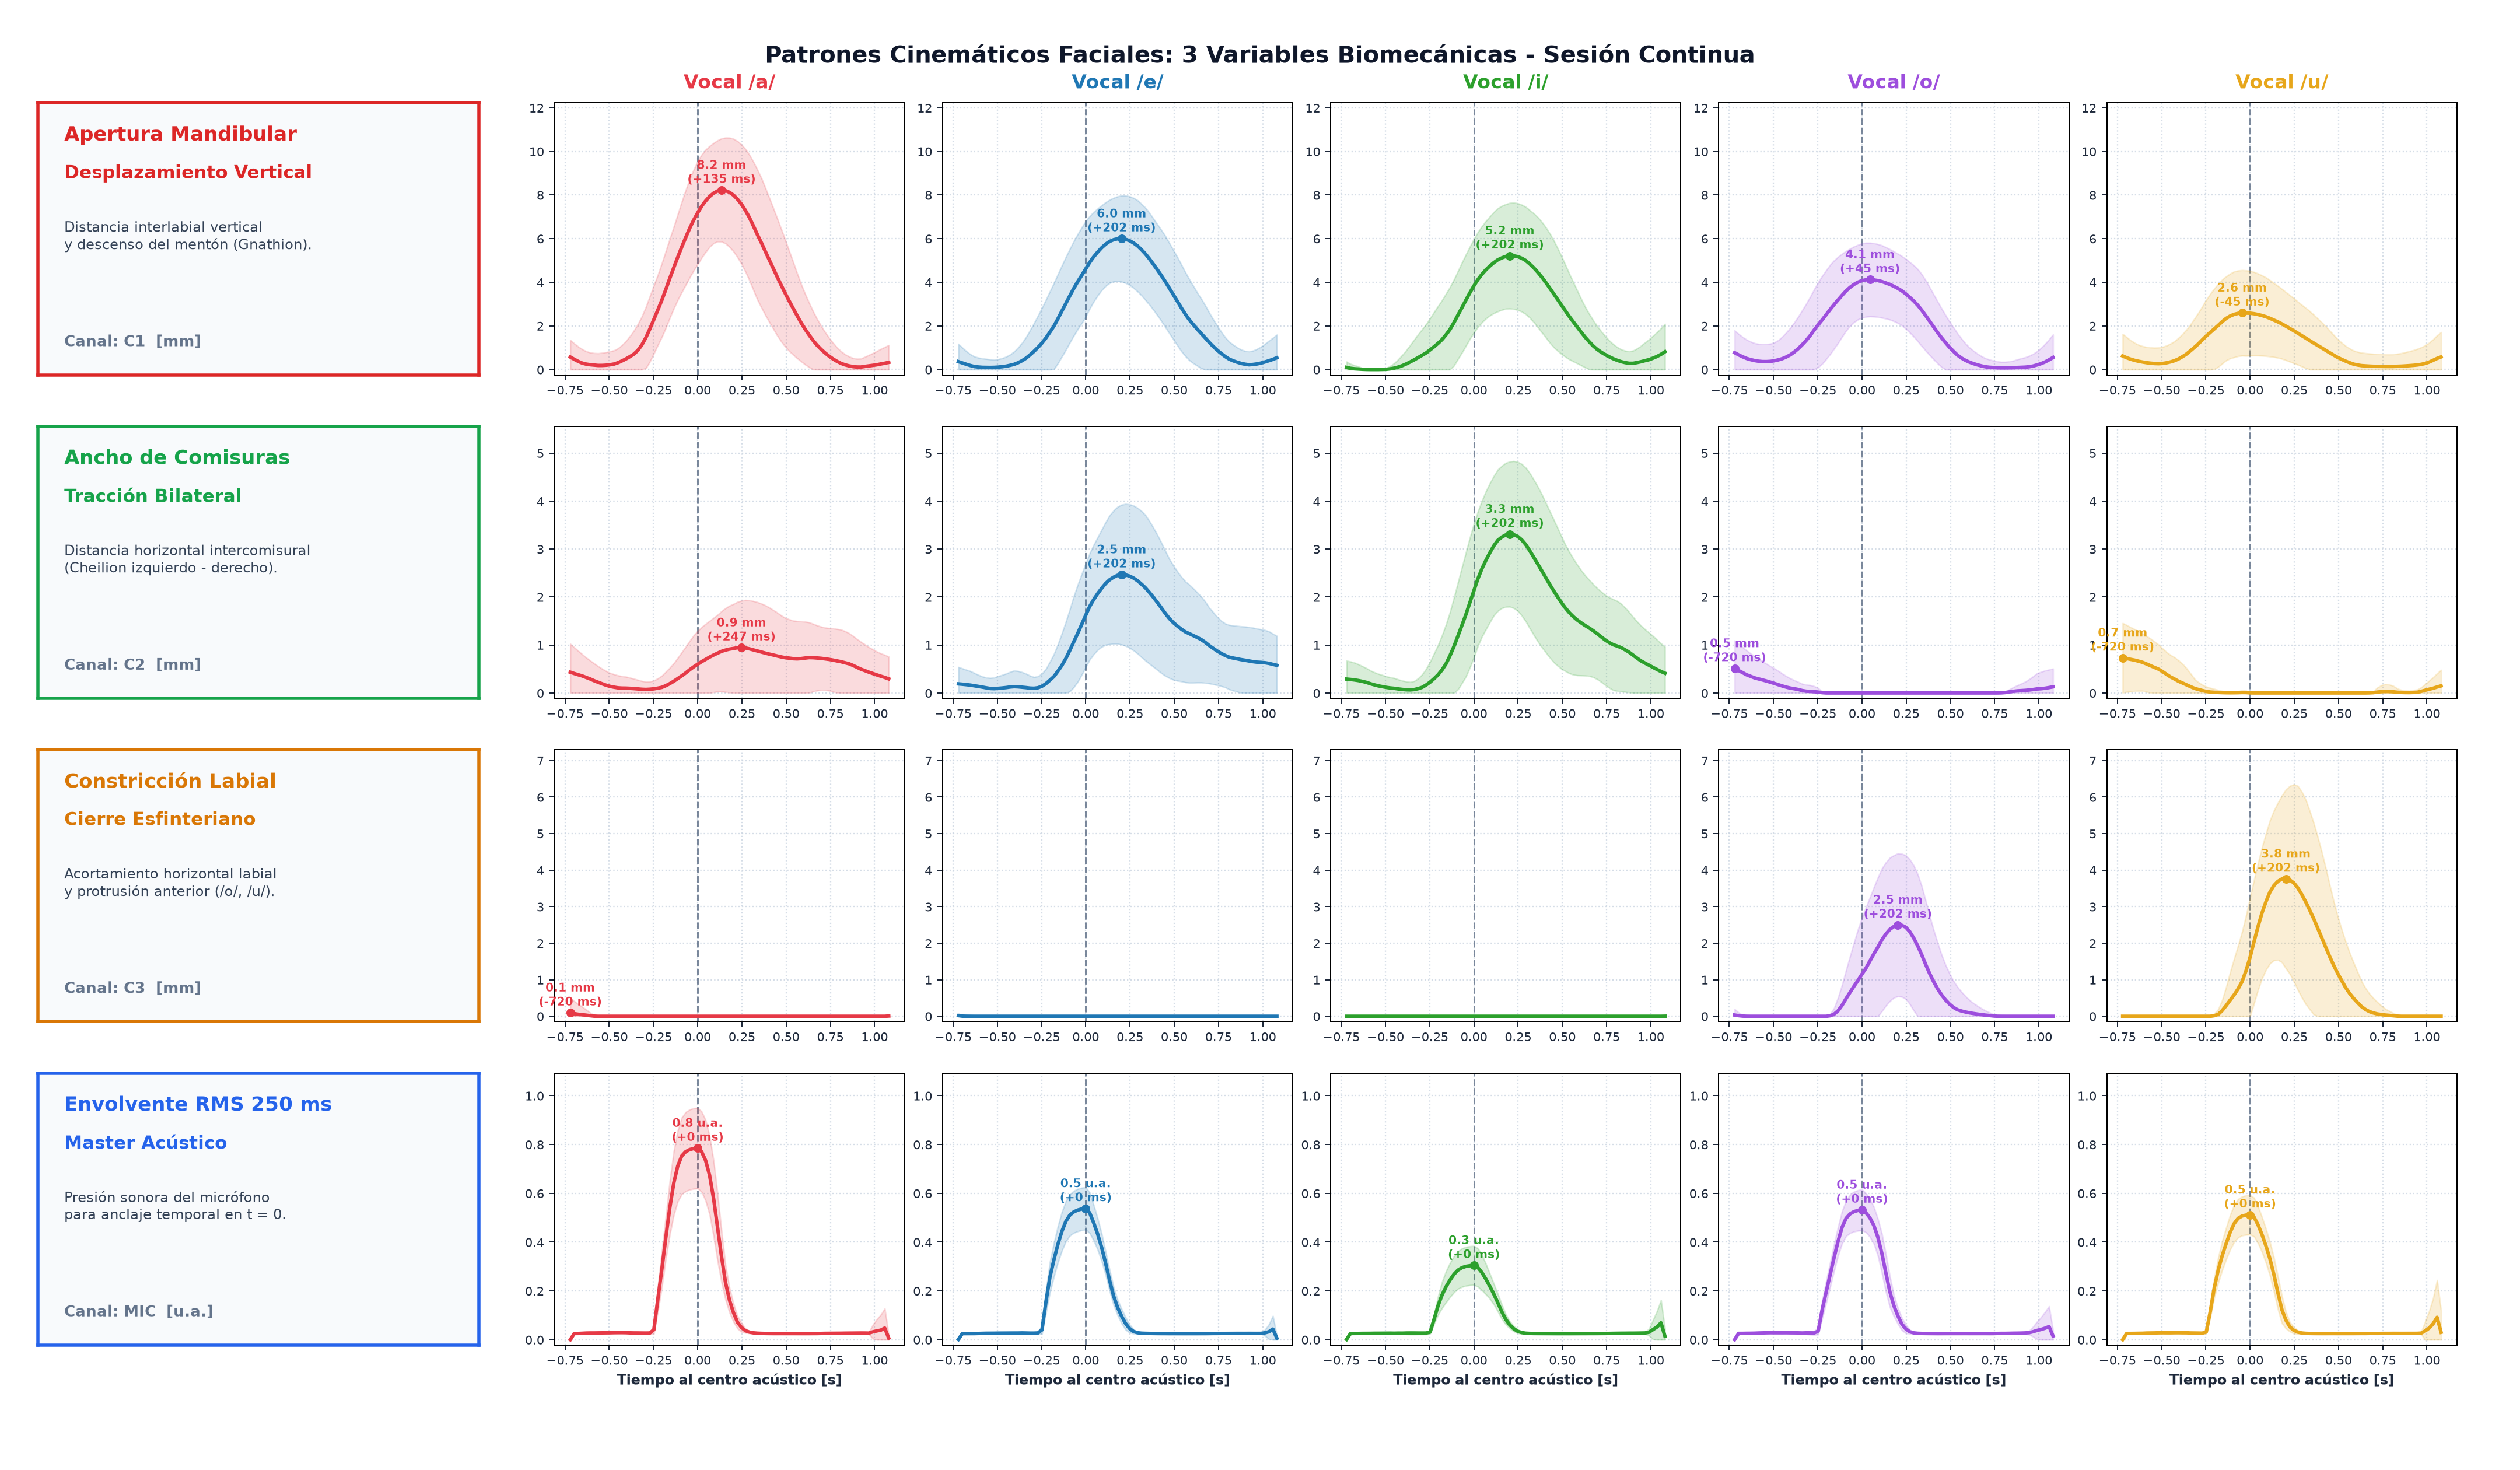
\includegraphics[width=0.98\textwidth]{figuras/exp3/patrones_cineticos_oficial.png}
    \caption{Patrones cinemáticos de 3 canales -- Experimento 3: Cadencia Rápida 40 BPM con Jitter del 20\% ($\tau \approx 1.80\,\text{s}$).}
    \label{fig:pat_3ch_exp3}
\end{figure}

\begin{figure}[htbp]
    \centering
    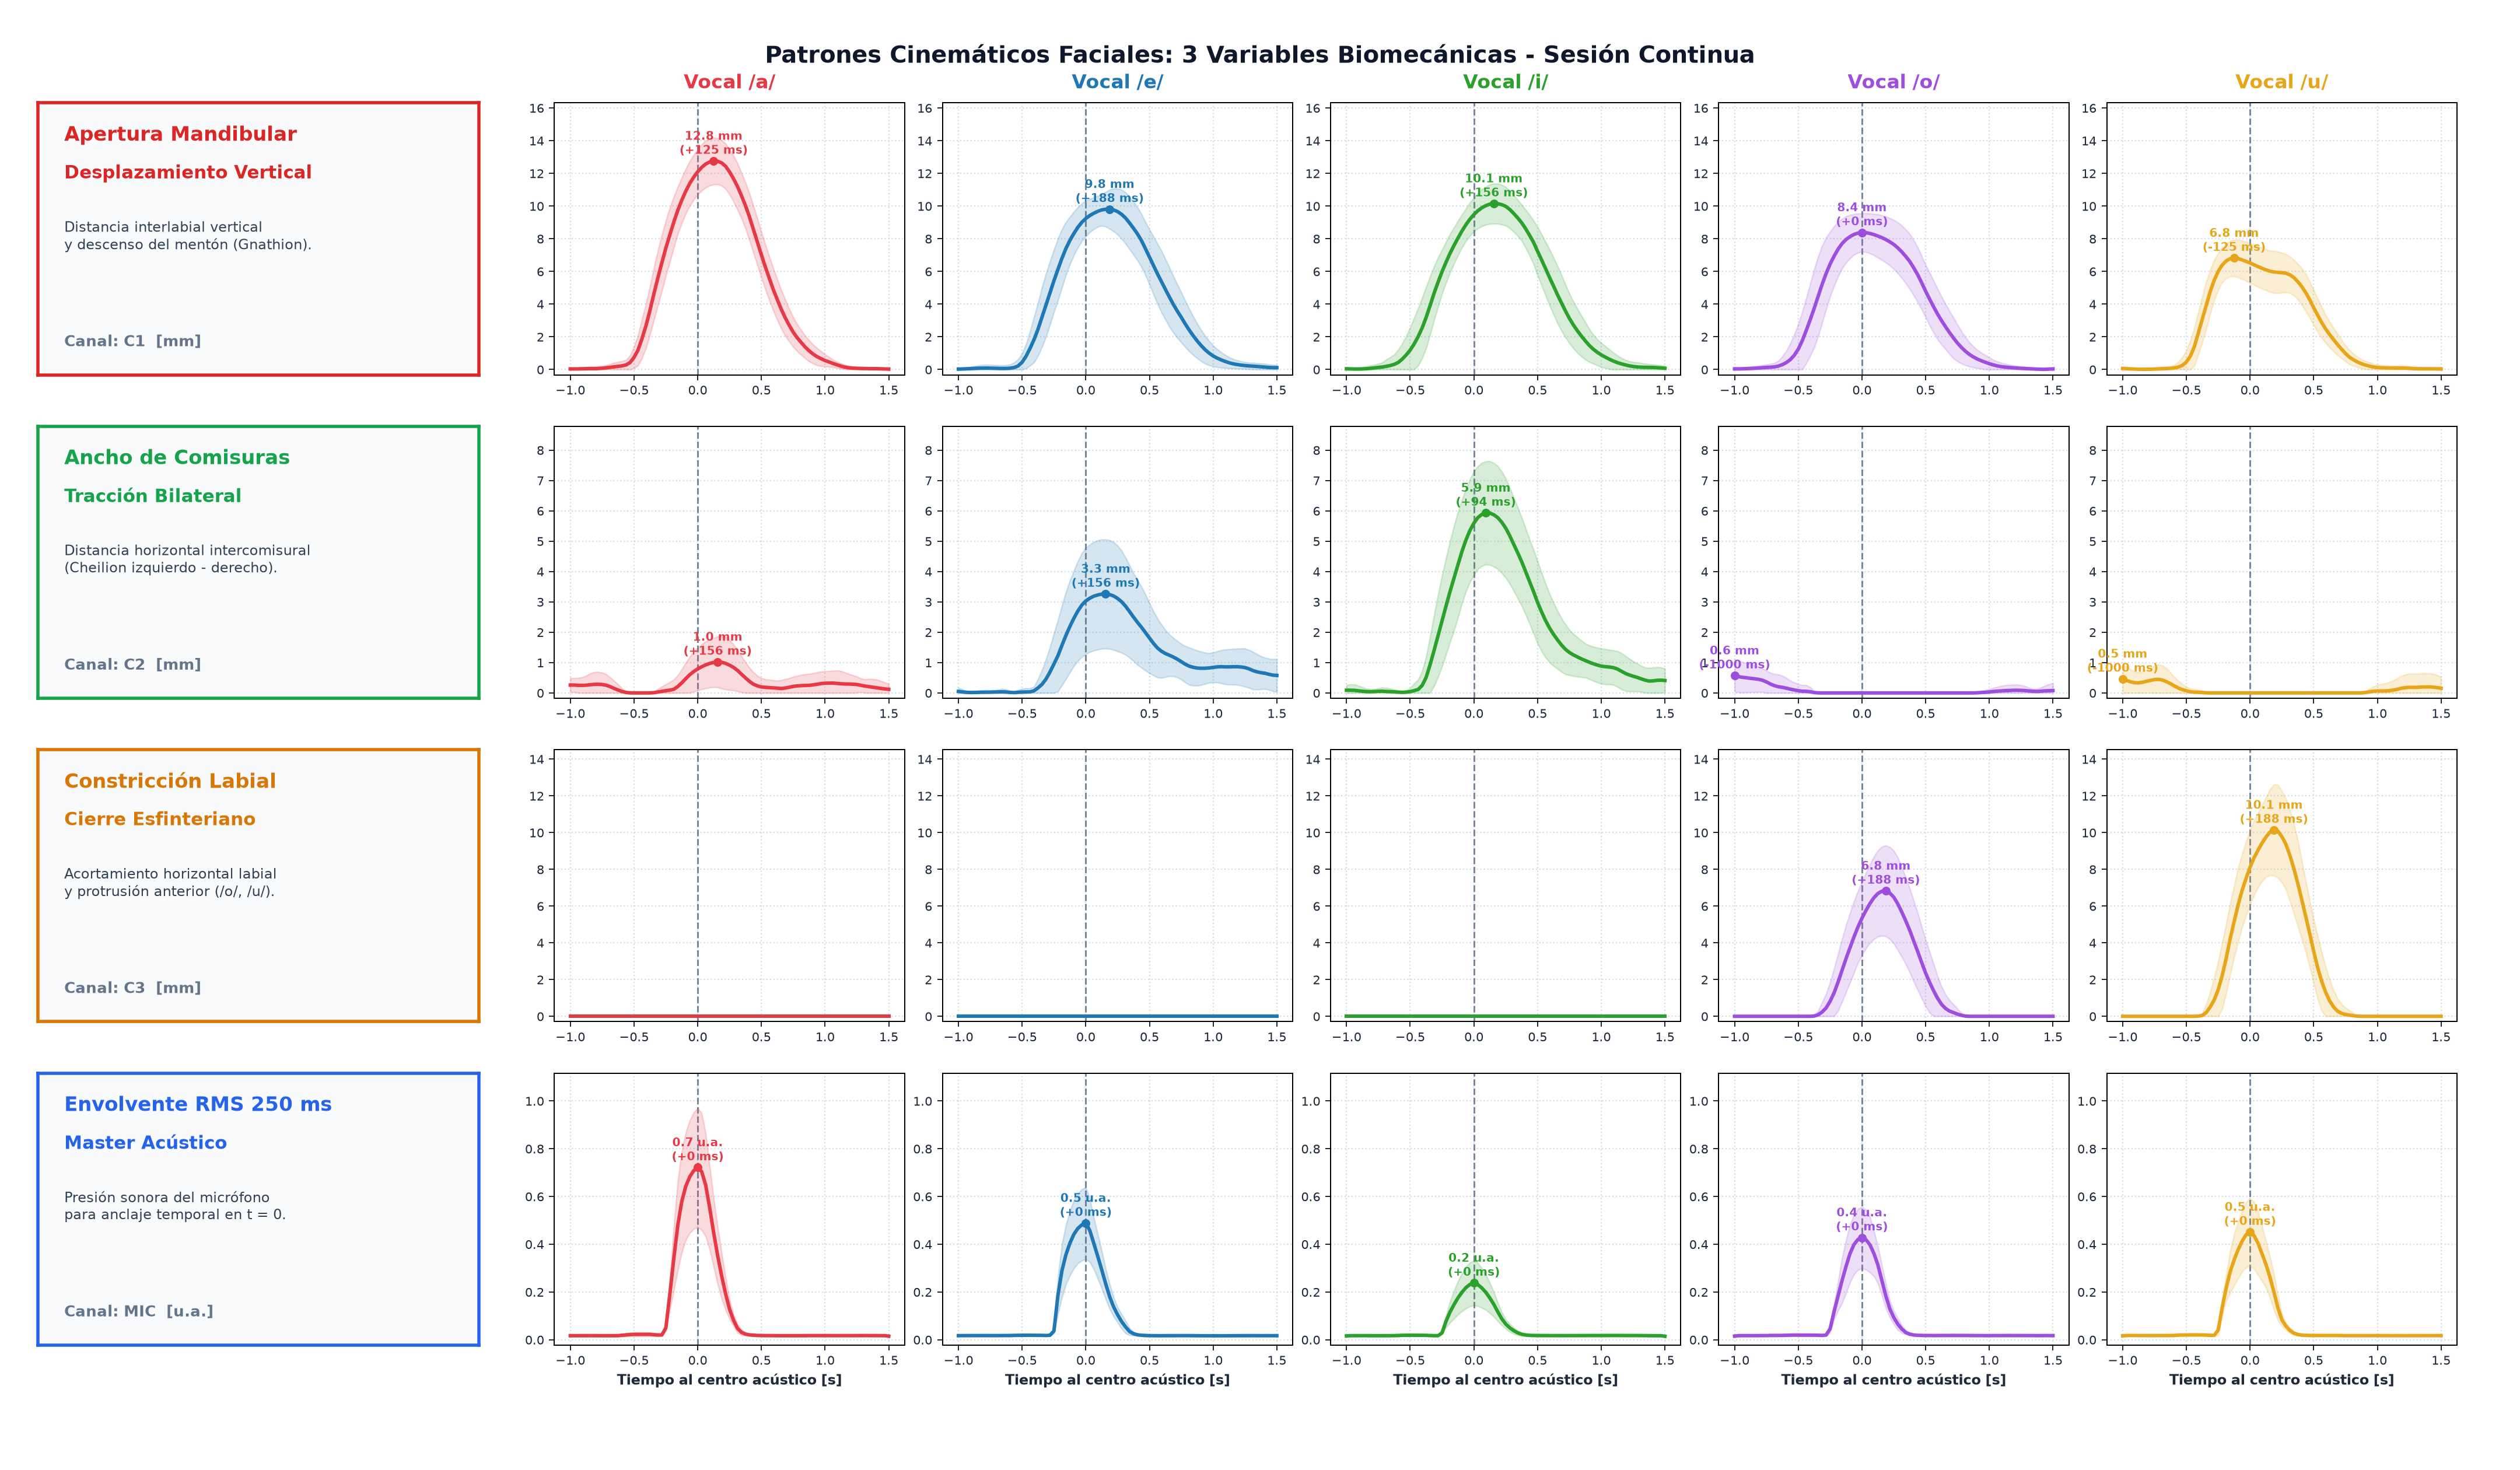
\includegraphics[width=0.98\textwidth]{figuras/exp4/patrones_cineticos_oficial.png}
    \caption{Patrones cinemáticos de 3 canales -- Experimento 4: Invarianza frente a perturbaciones de distancia focal y rotación cefálica ($\tau = 2.50\,\text{s}$).}
    \label{fig:pat_3ch_exp4}
\end{figure}

\newpage
\section{Patrones Cinemáticos de Activación (6 Canales Bio-Inspirados)}
Expansión dimensional completa a 6 variables fisiológicas (apertura mandibular, tracción cigomática, constricción esfinteriana, retracción de mejilla, ascenso malar y compresión maseterina).

\begin{figure}[htbp]
    \centering
    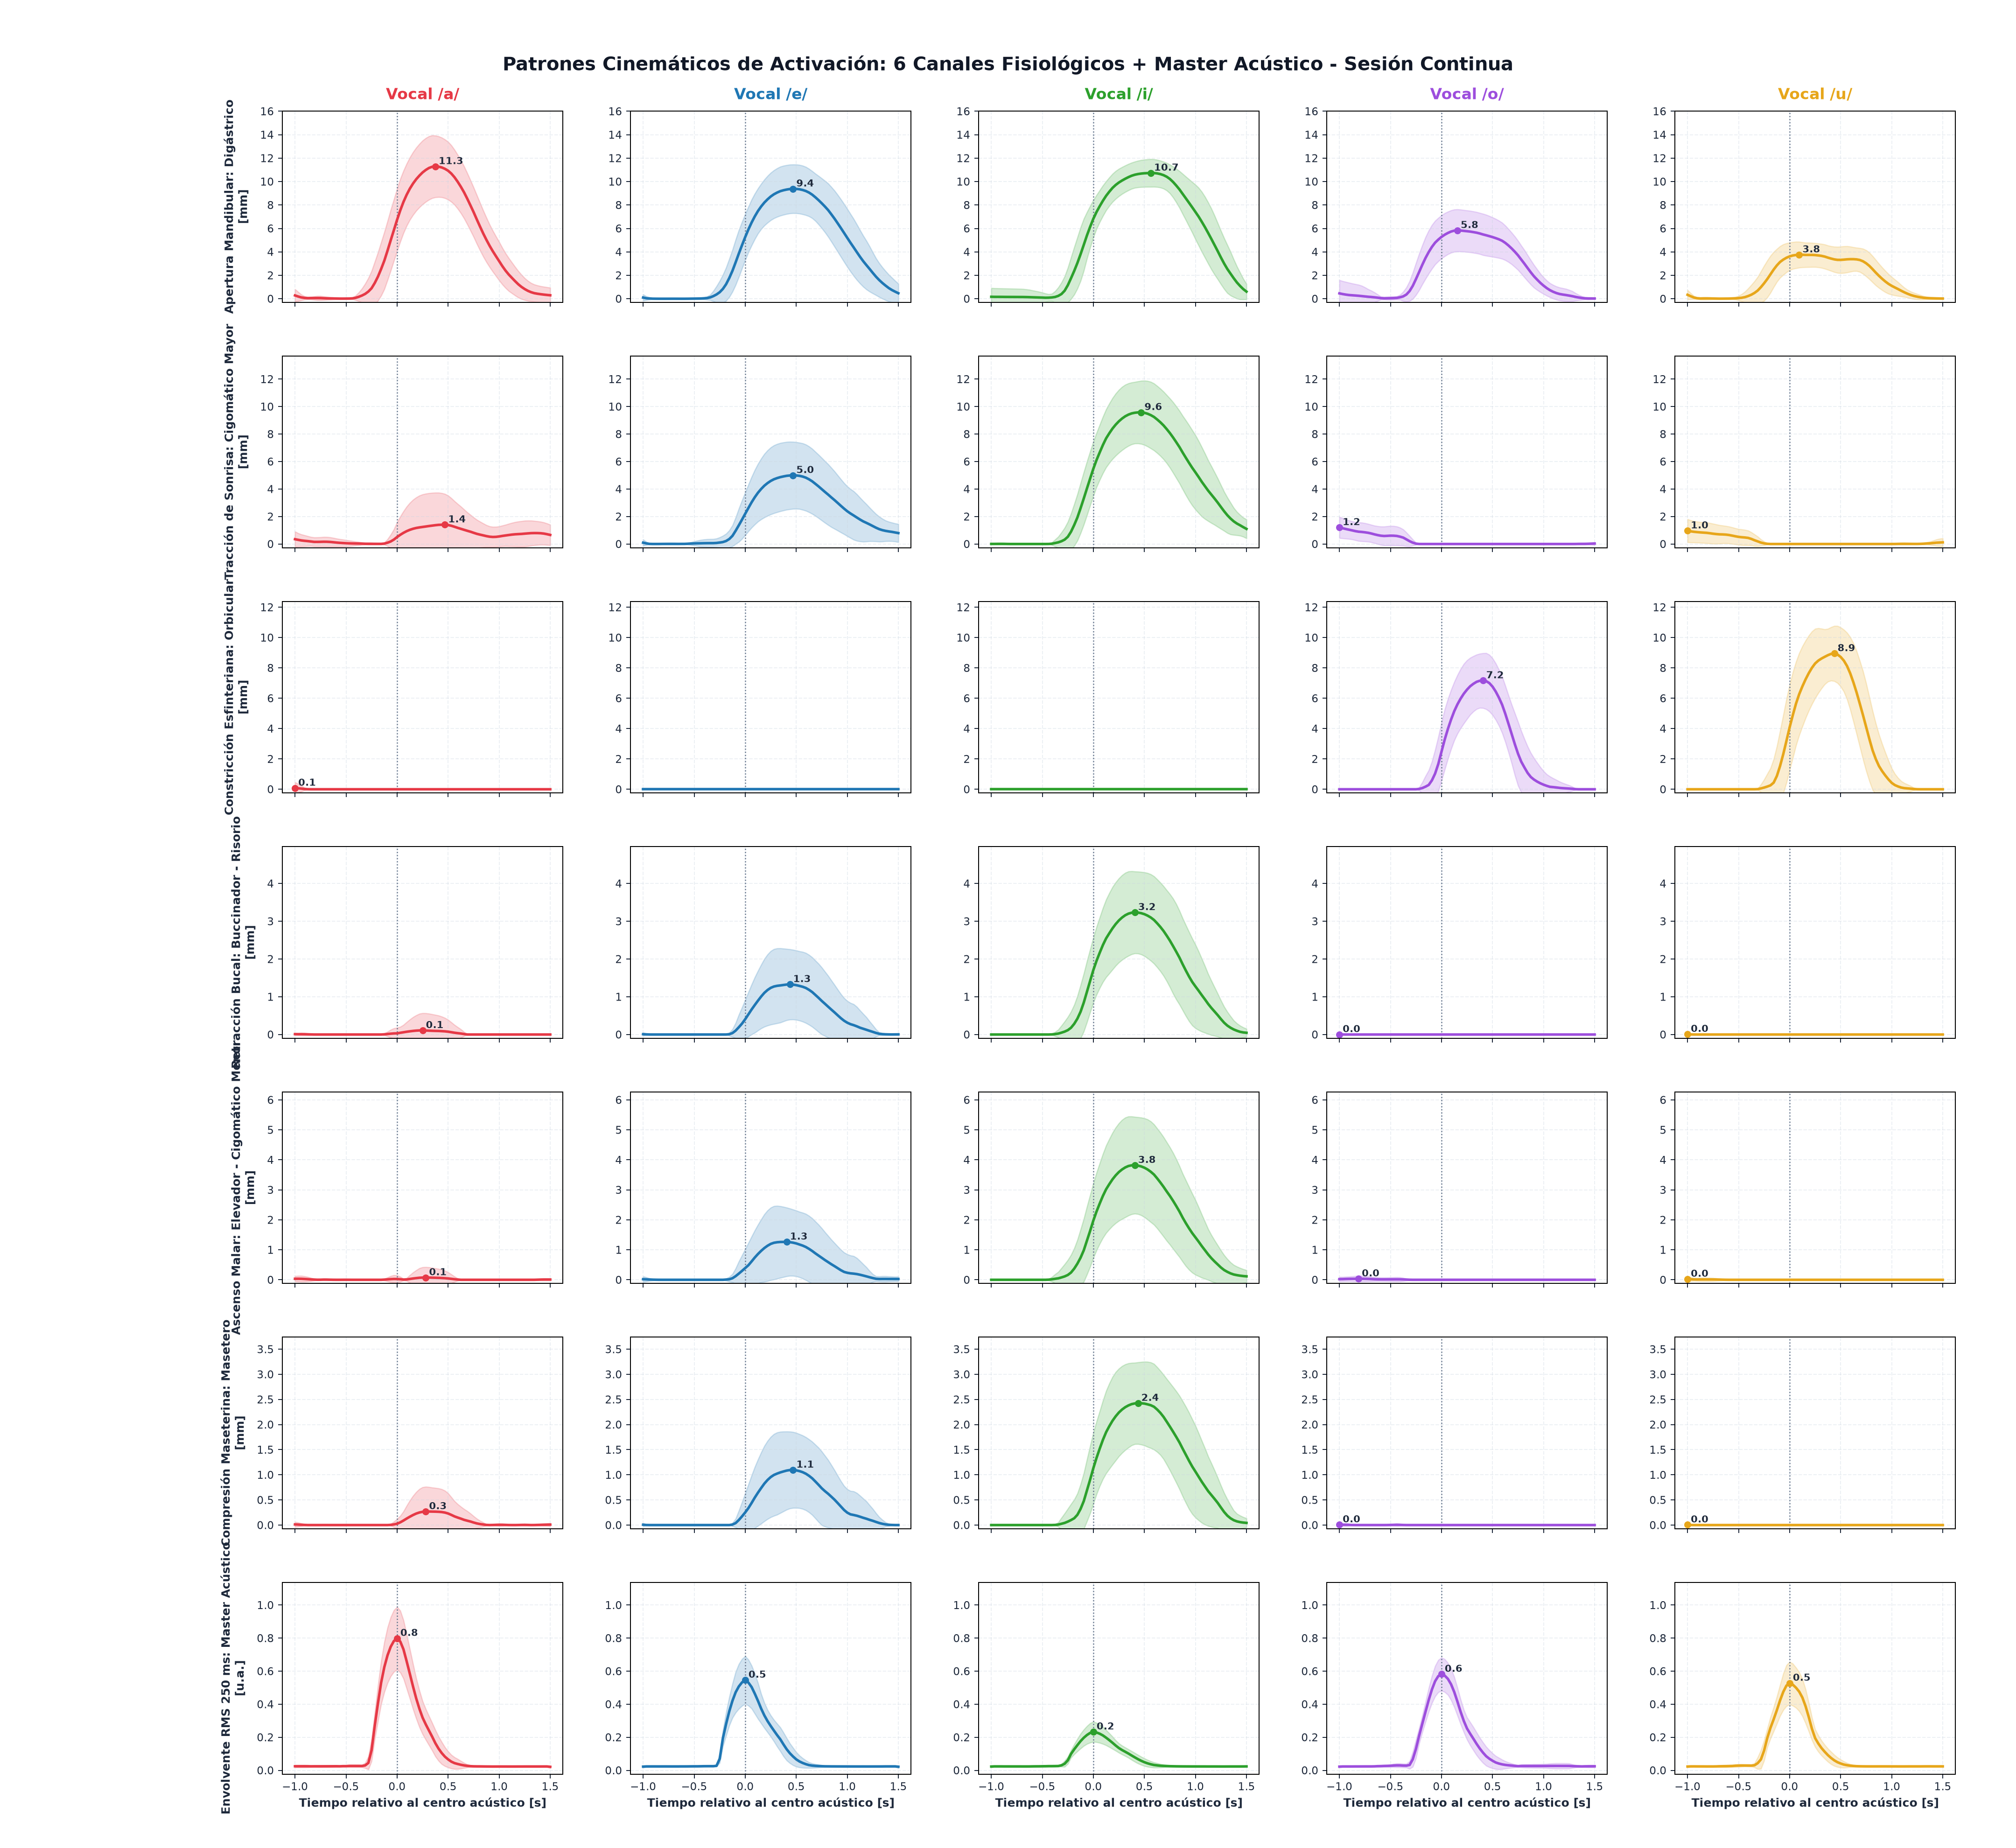
\includegraphics[width=0.95\textwidth]{figuras/exp1/patrones_6canales_oficial.png}
    \caption{Patrones de 6 canales -- Experimento 1: Hiperarticulado 24 BPM.}
    \label{fig:pat_6ch_exp1}
\end{figure}

\begin{figure}[htbp]
    \centering
    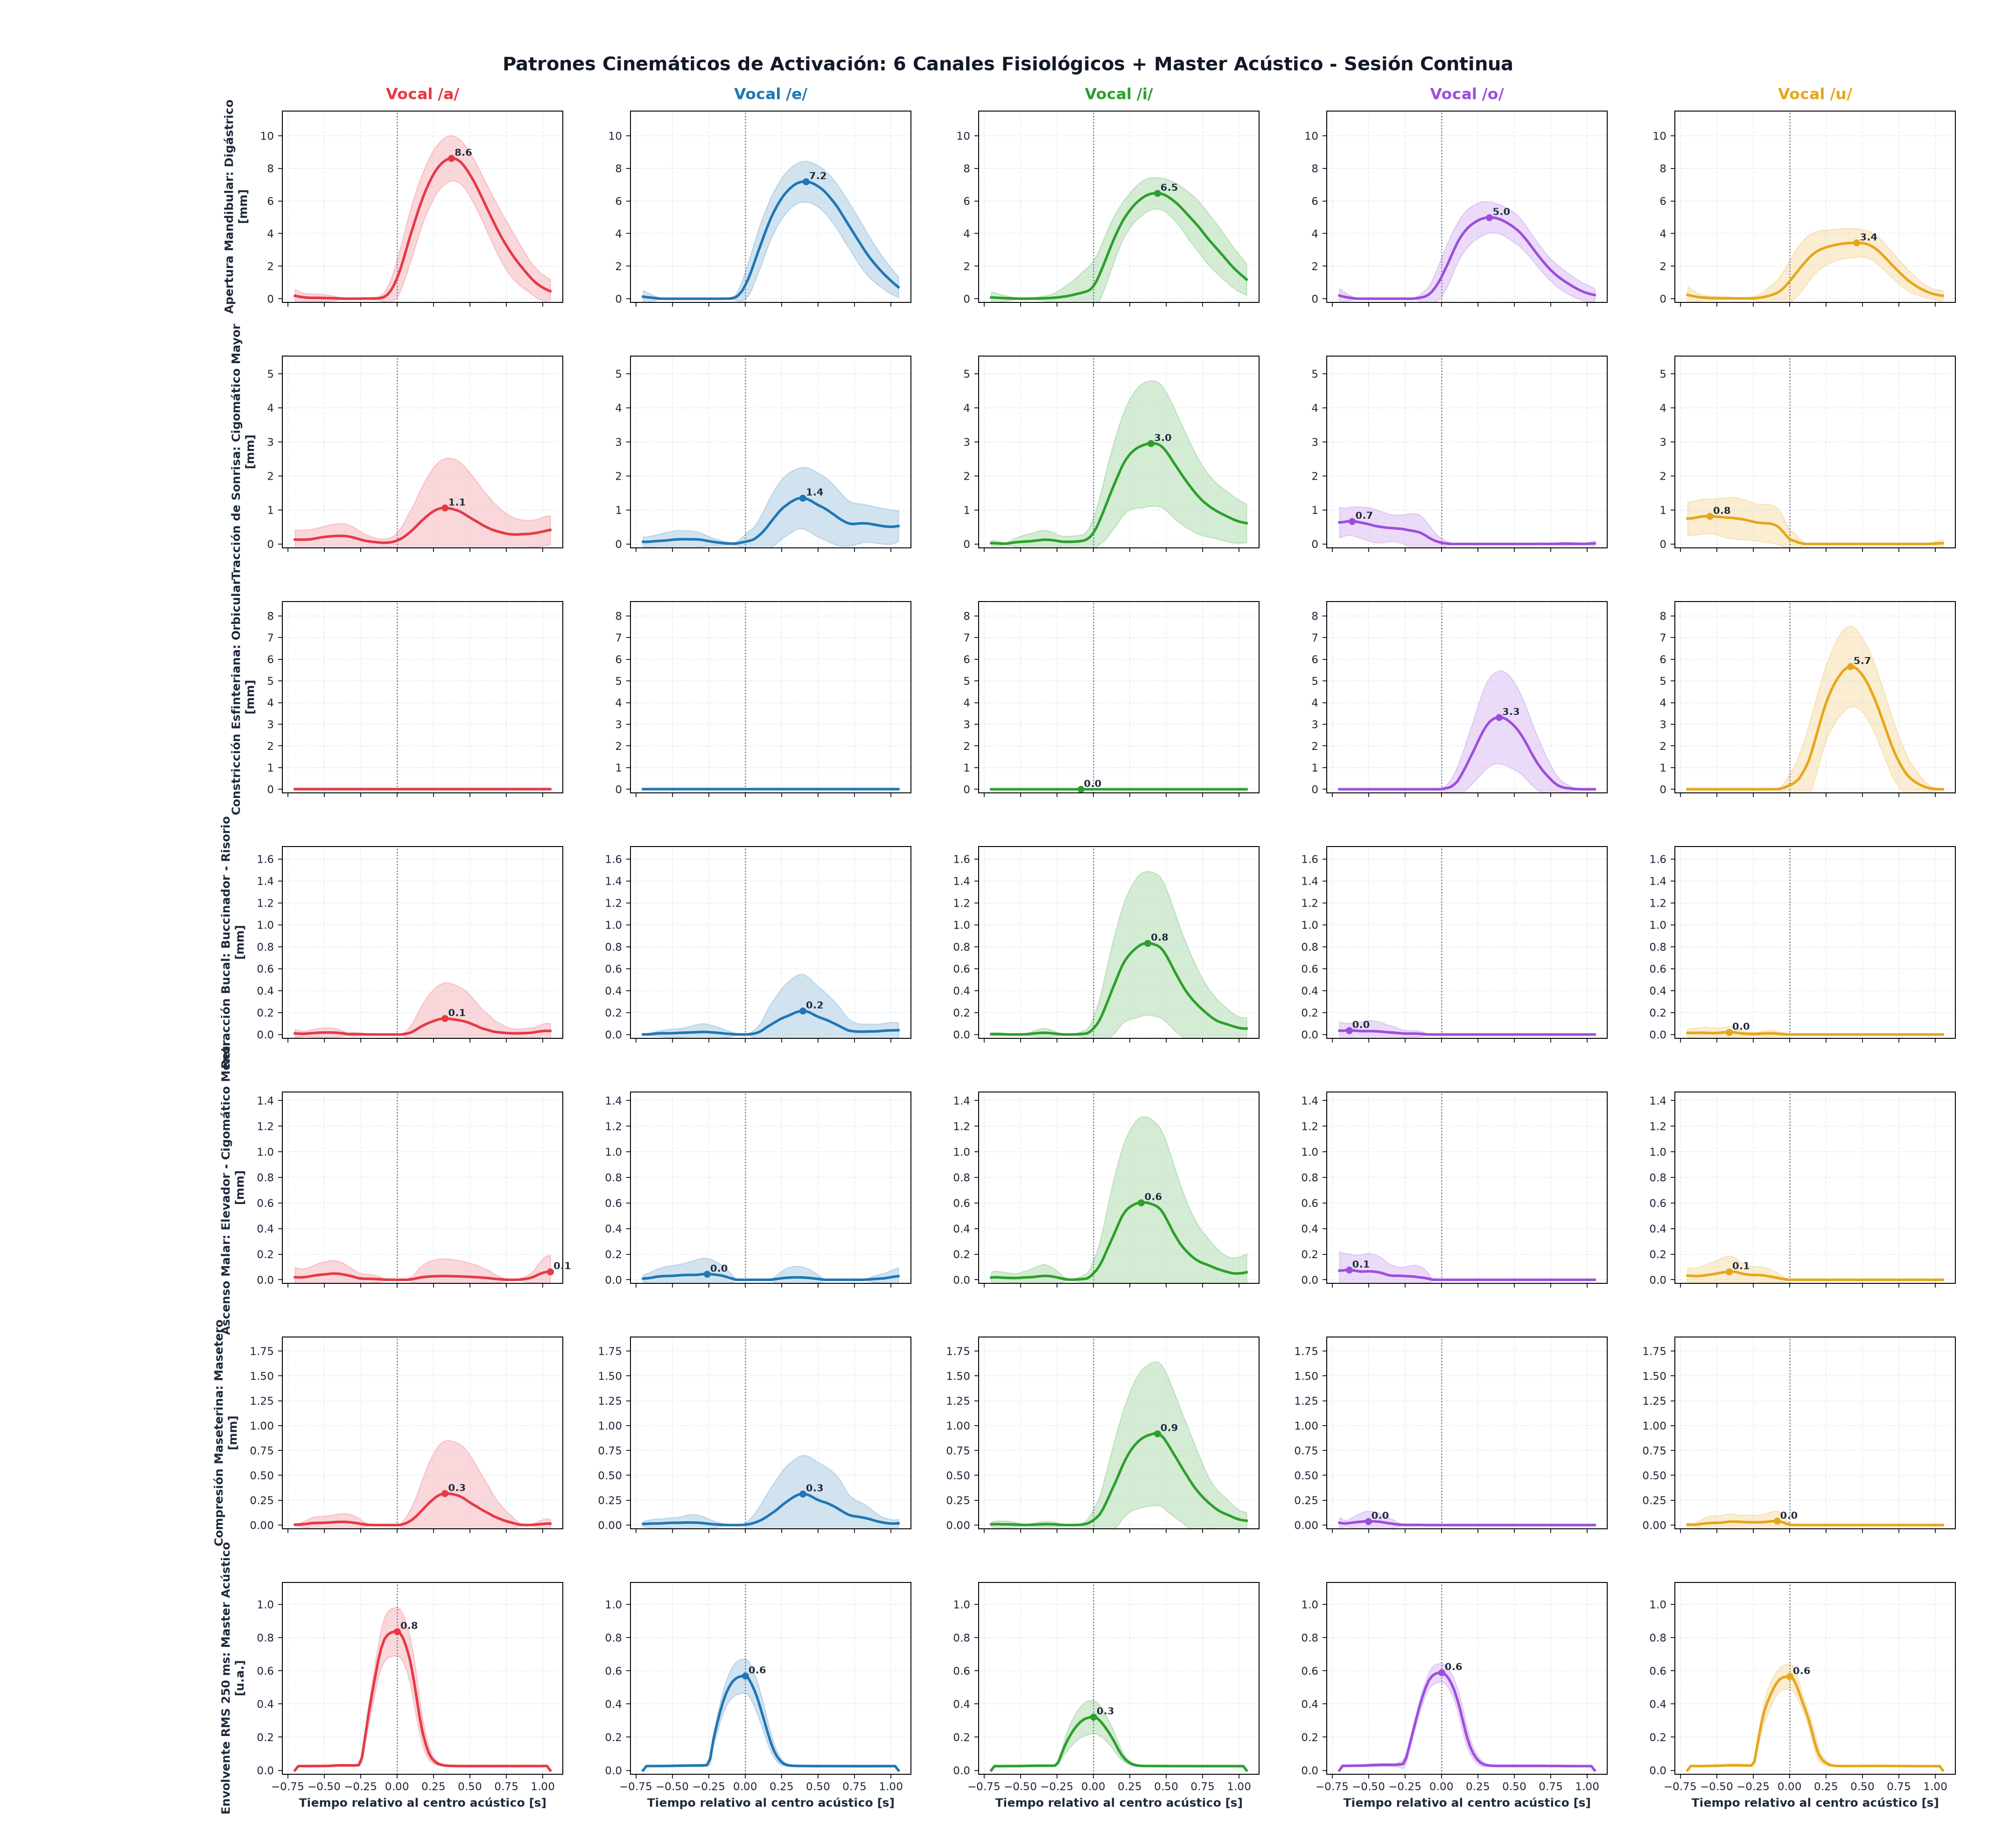
\includegraphics[width=0.95\textwidth]{figuras/exp2/patrones_6canales_oficial.png}
    \caption{Patrones de 6 canales -- Experimento 2: Cadencia Natural 30 BPM Jitter 15\%.}
    \label{fig:pat_6ch_exp2}
\end{figure}

\begin{figure}[htbp]
    \centering
    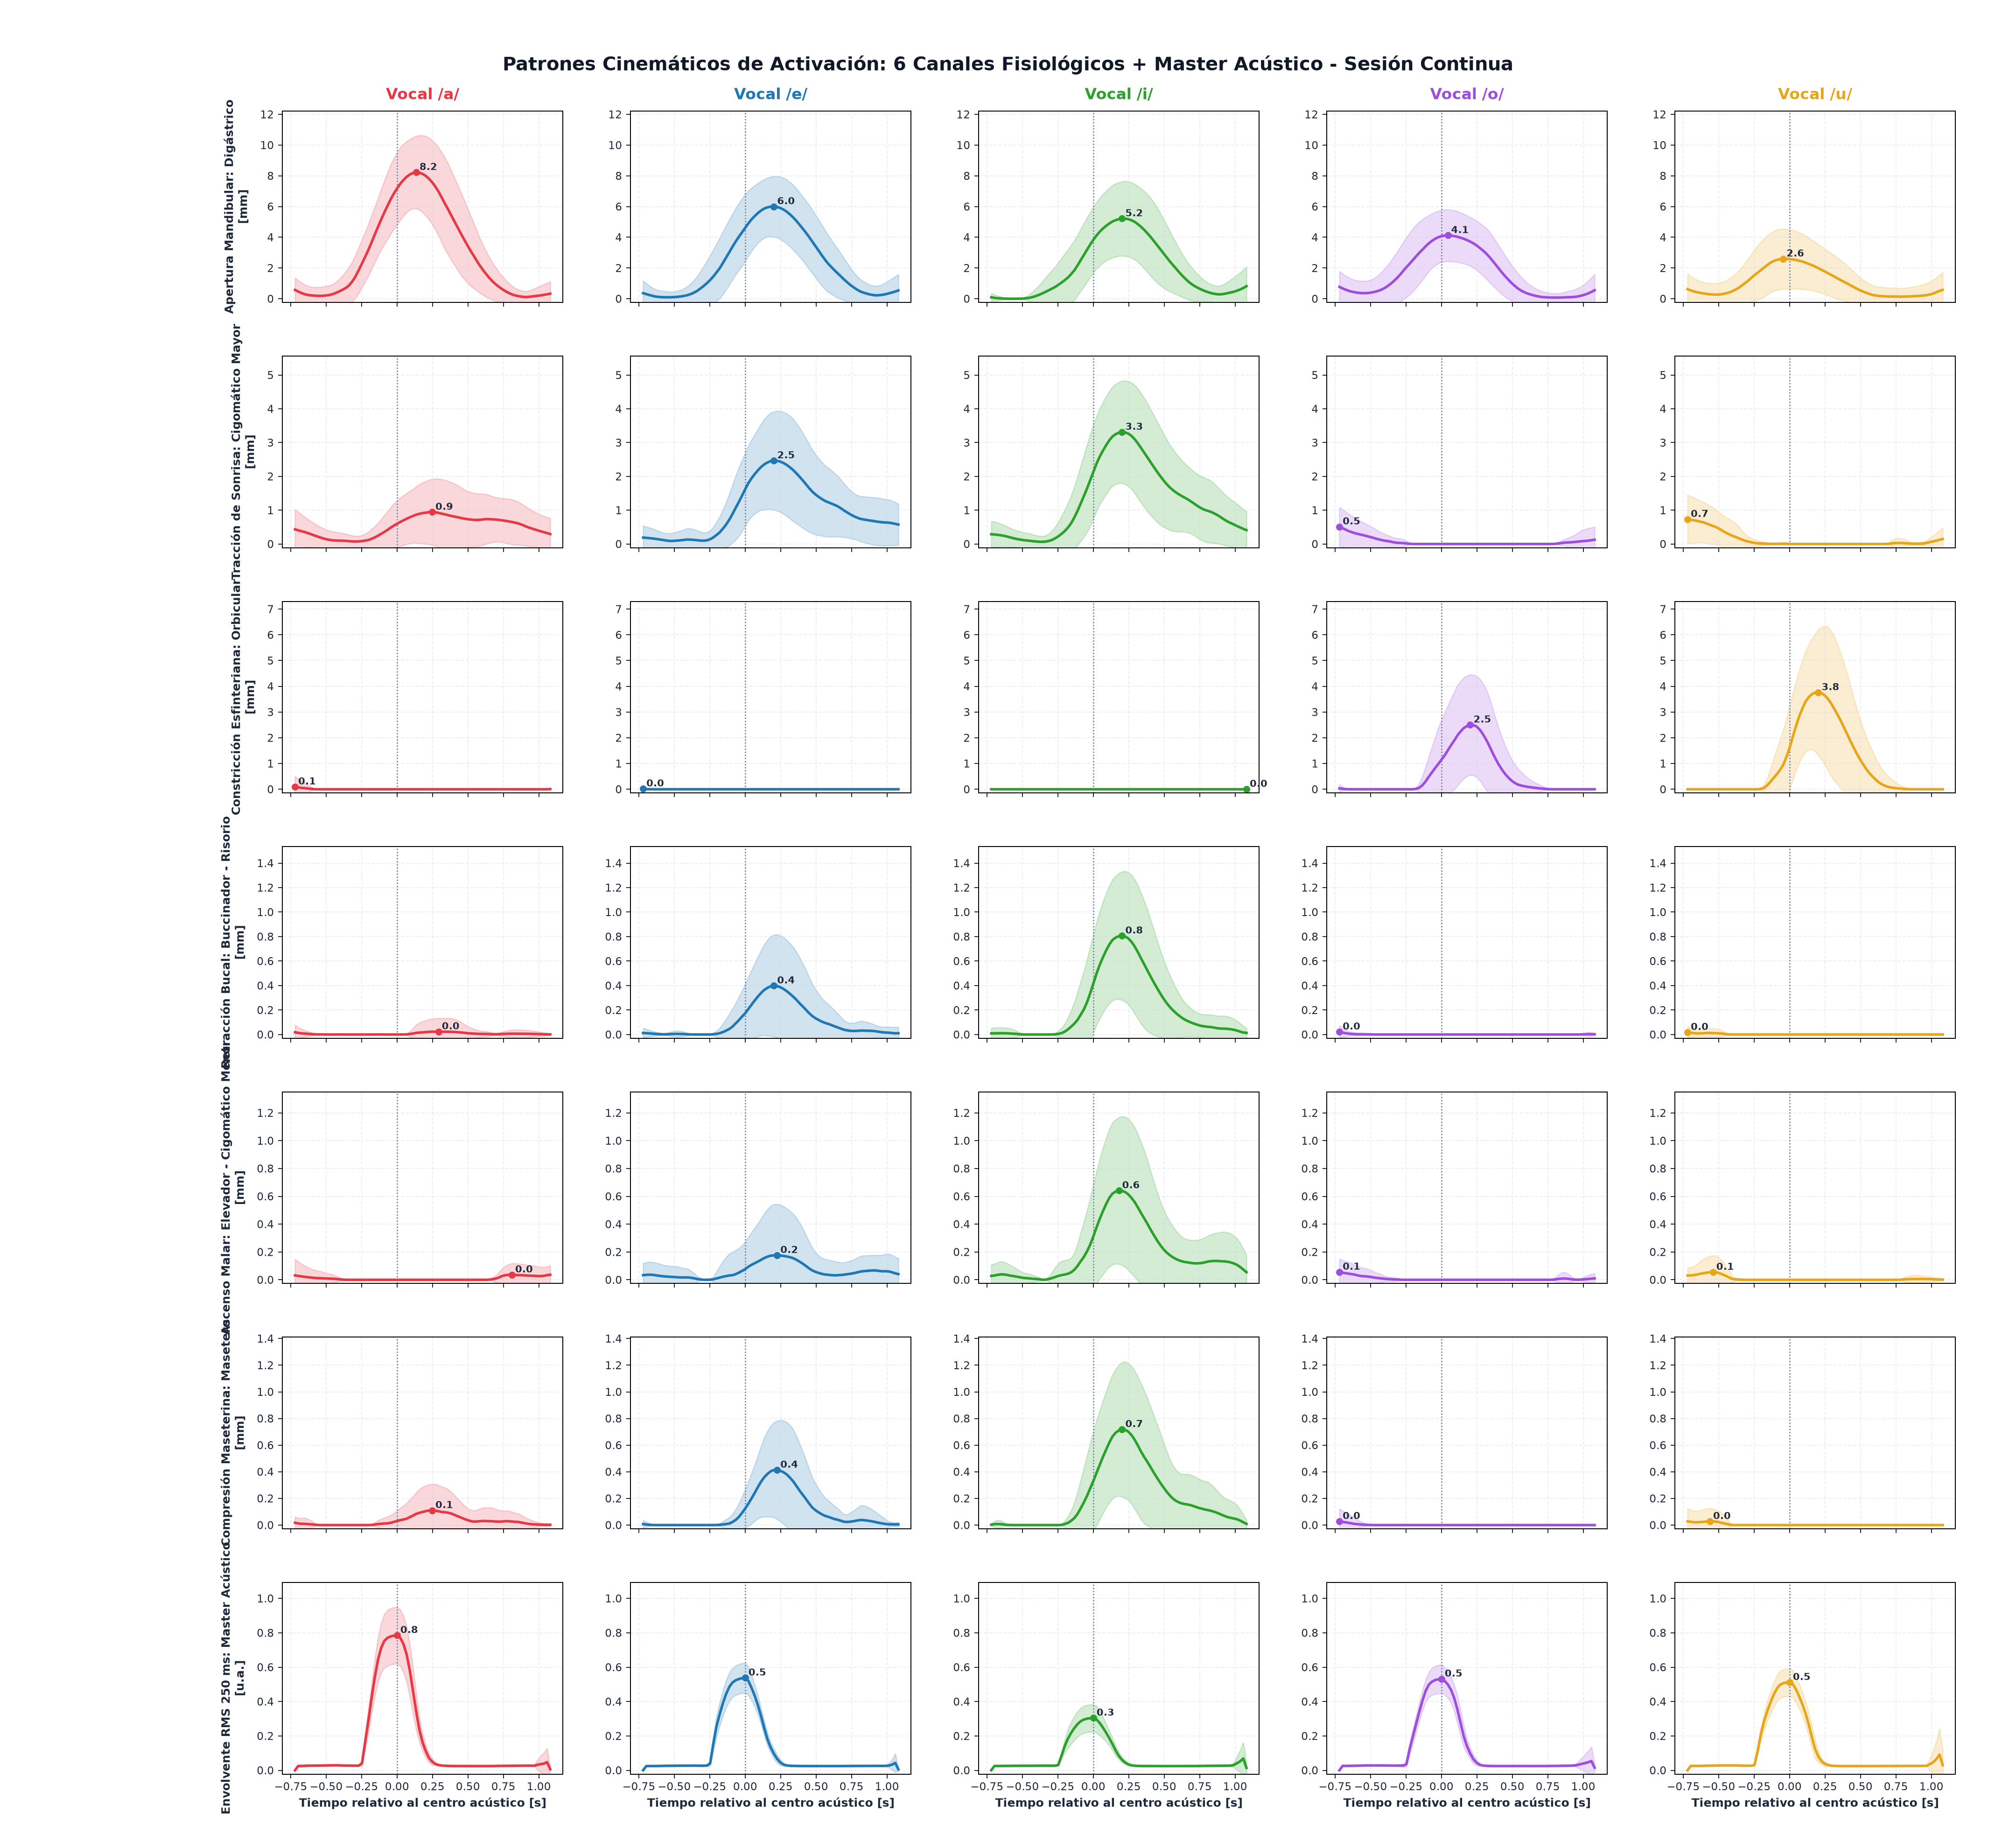
\includegraphics[width=0.95\textwidth]{figuras/exp3/patrones_6canales_oficial.png}
    \caption{Patrones de 6 canales -- Experimento 3: Cadencia Rápida 40 BPM Jitter 20\%.}
    \label{fig:pat_6ch_exp3}
\end{figure}

\begin{figure}[htbp]
    \centering
    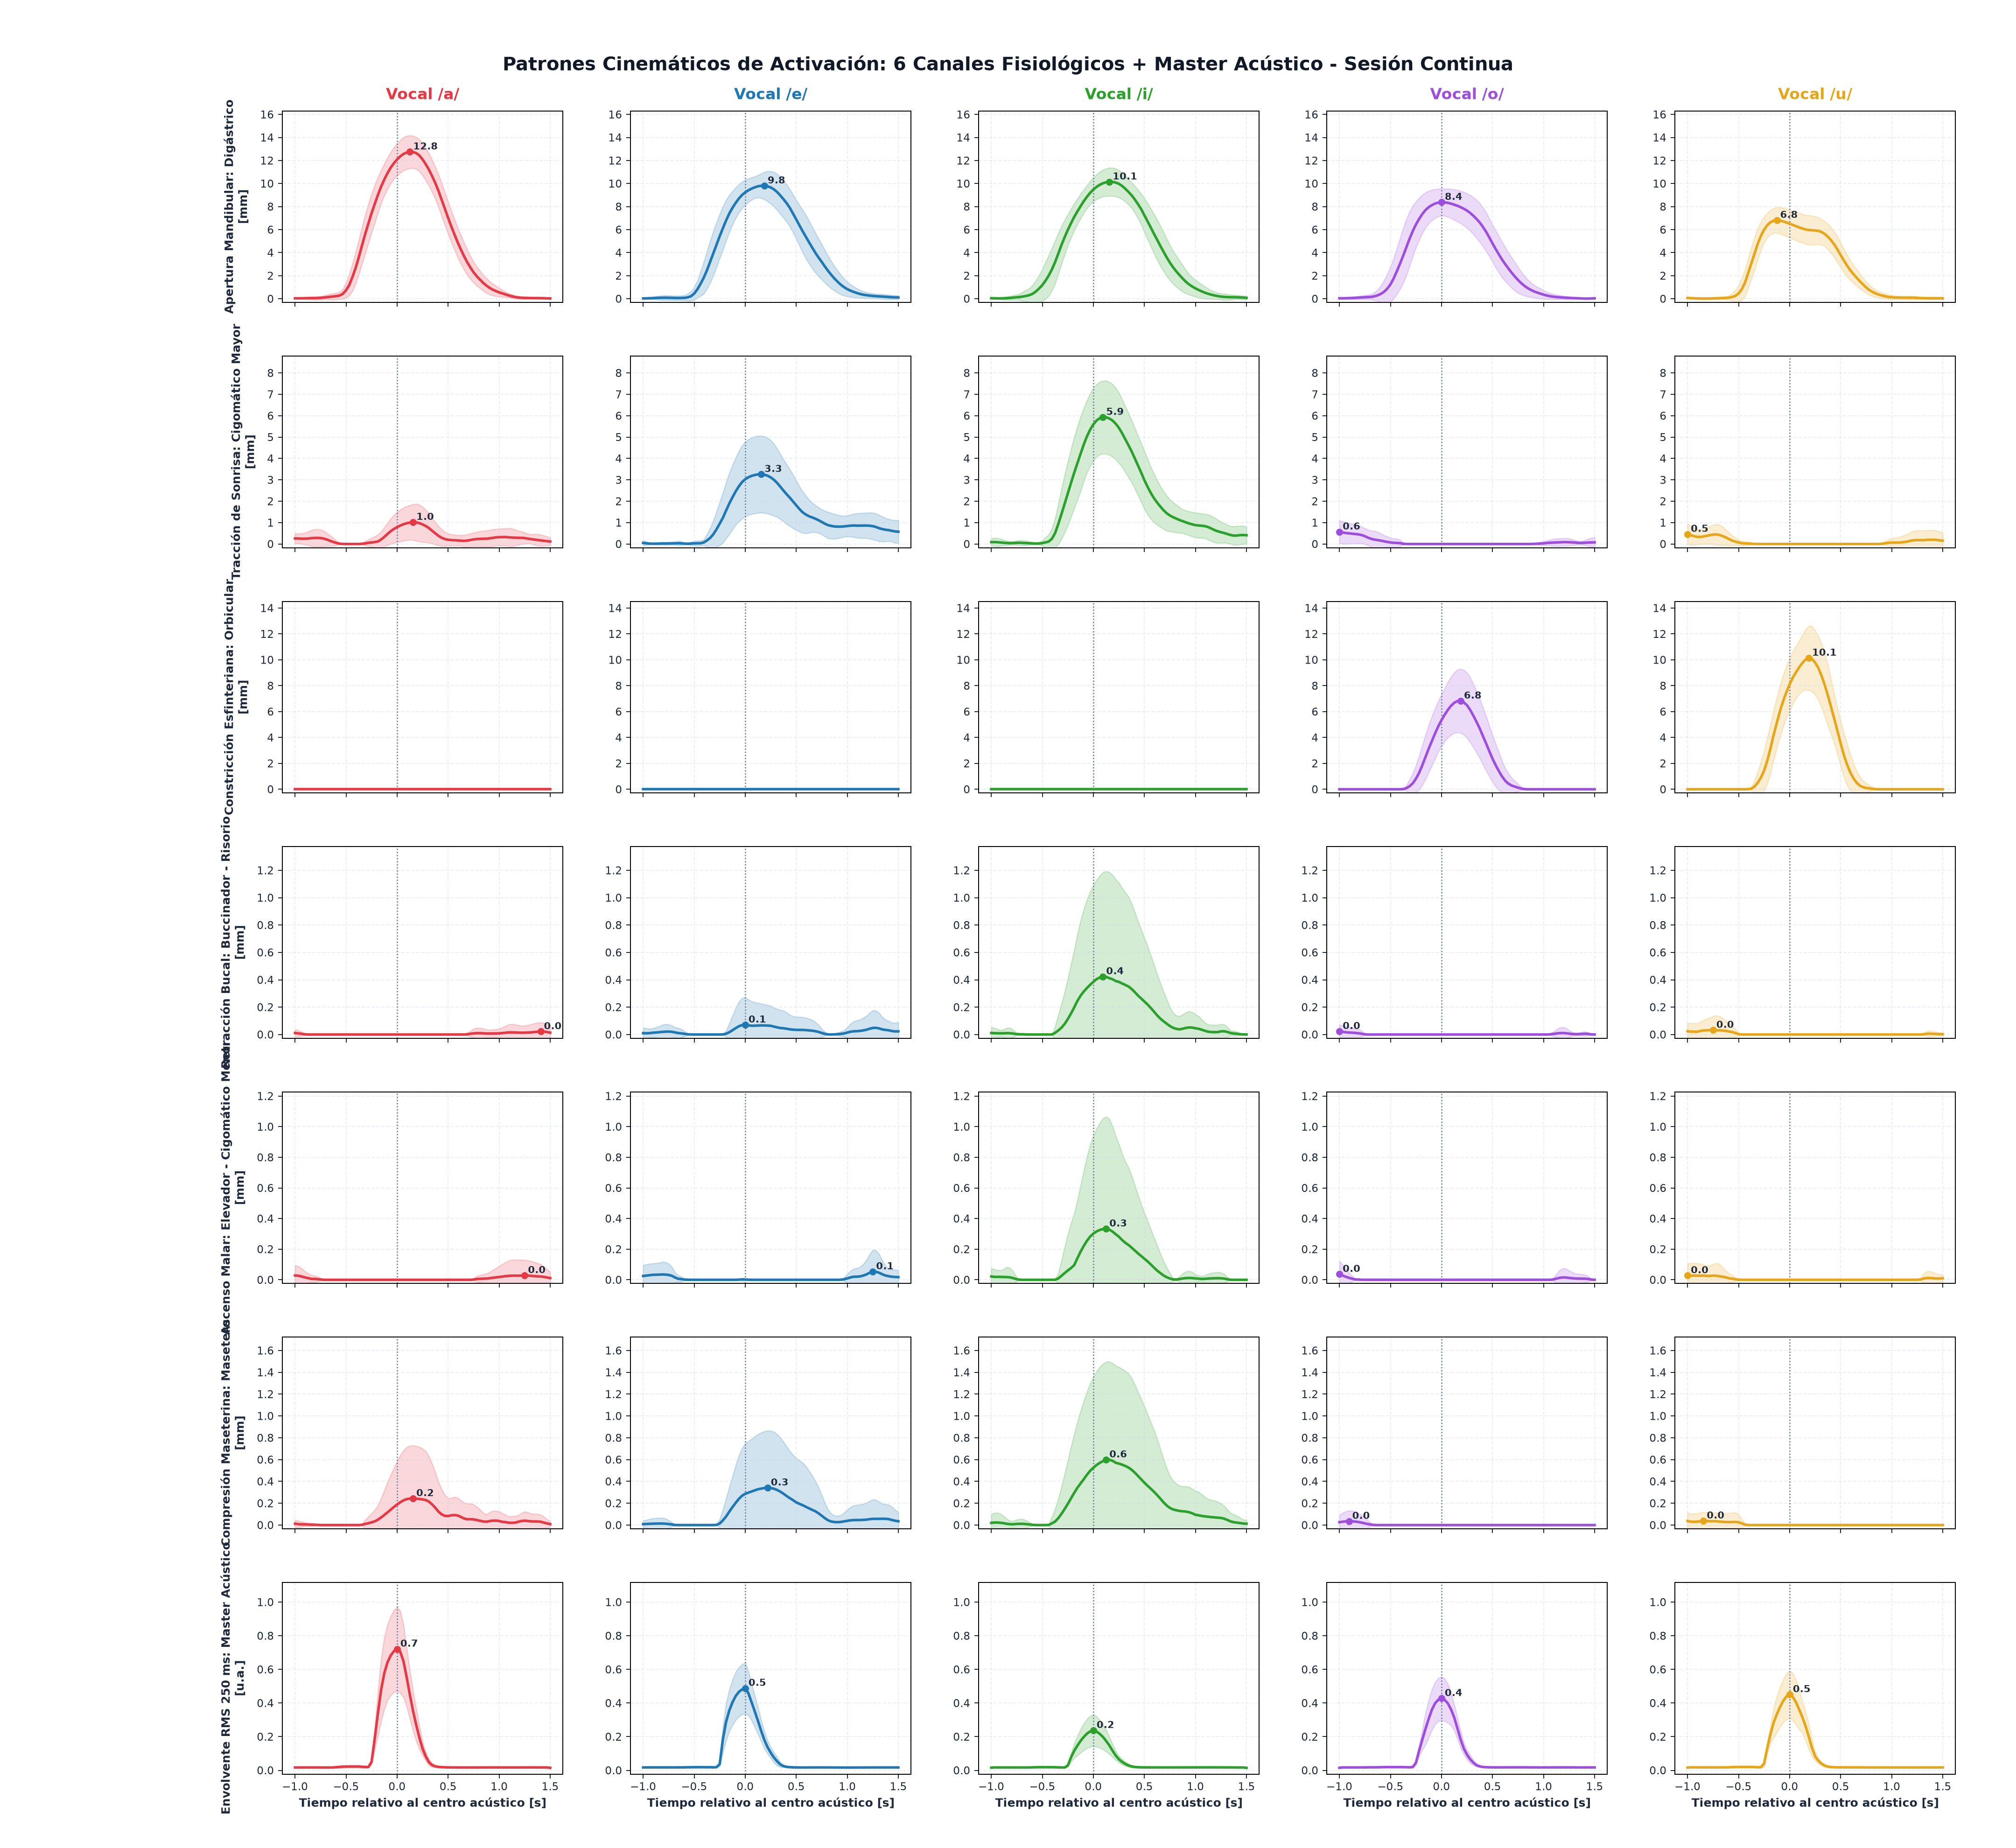
\includegraphics[width=0.95\textwidth]{figuras/exp4/patrones_6canales_oficial.png}
    \caption{Patrones de 6 canales -- Experimento 4: Invarianza de Distancia y Pose.}
    \label{fig:pat_6ch_exp4}
\end{figure}

\newpage
\section{Topología Acústica: Planos Formánticos F1 vs F2}
Planos de dispersión formántica tradicional ($F_1$ vs $F_2$ en escala Hertz invertida) calculados mediante codificación predictiva lineal (LPC de orden 12) sobre el micrófono maestro a $44.1\,\text{kHz}$.

\begin{figure}[htbp]
    \centering
    \begin{subfigure}[b]{0.48\textwidth}
        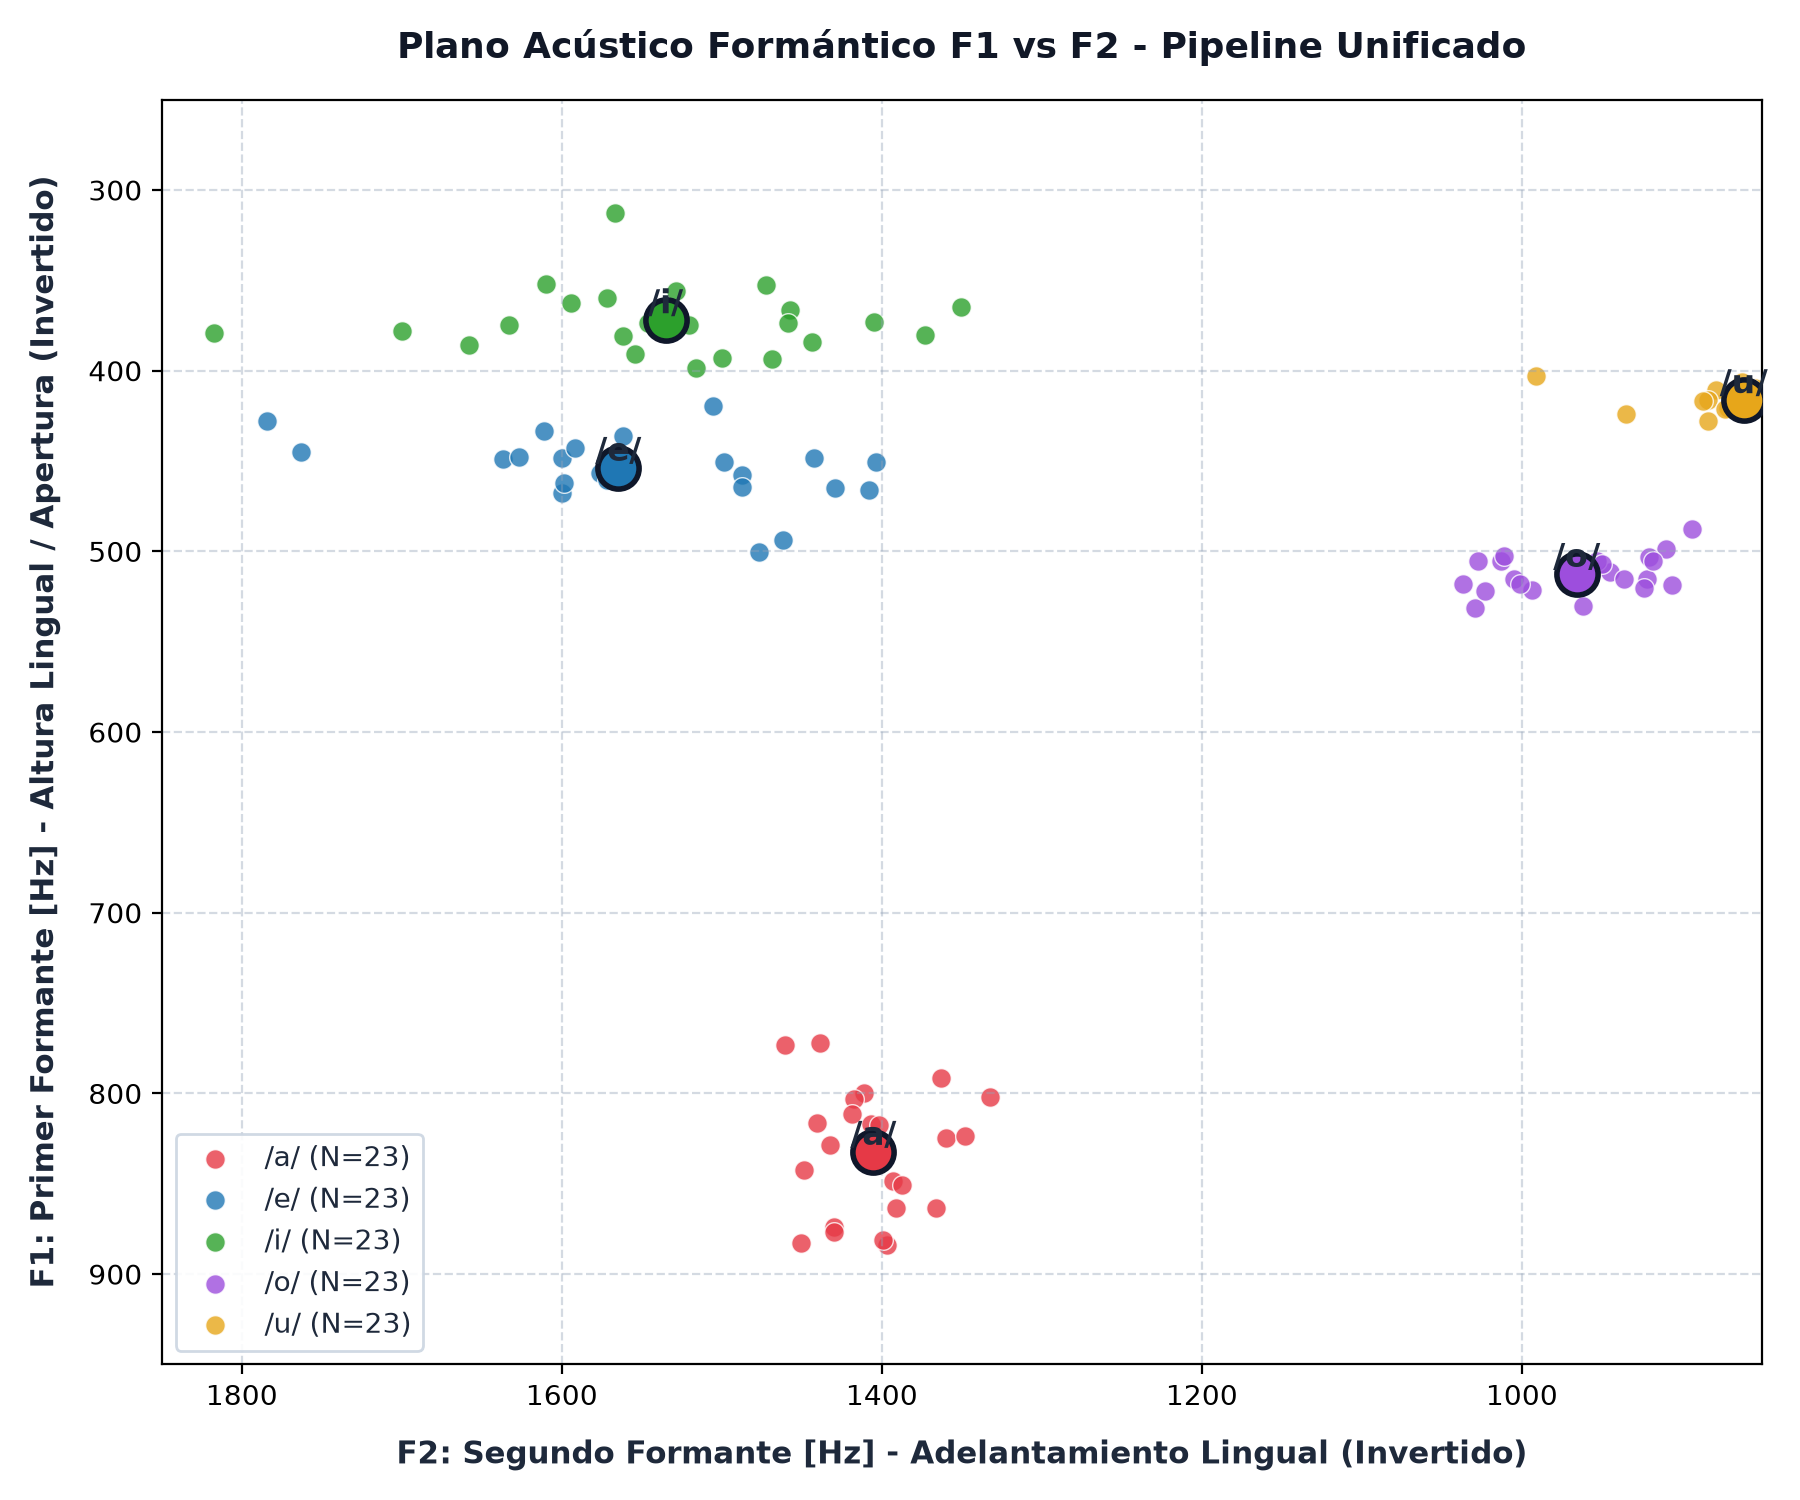
\includegraphics[width=\textwidth]{figuras/exp1/plano_formantes_lineal.png}
        \caption{Exp. 1: Hiperarticulado 24 BPM}
    \end{subfigure}
    \hfill
    \begin{subfigure}[b]{0.48\textwidth}
        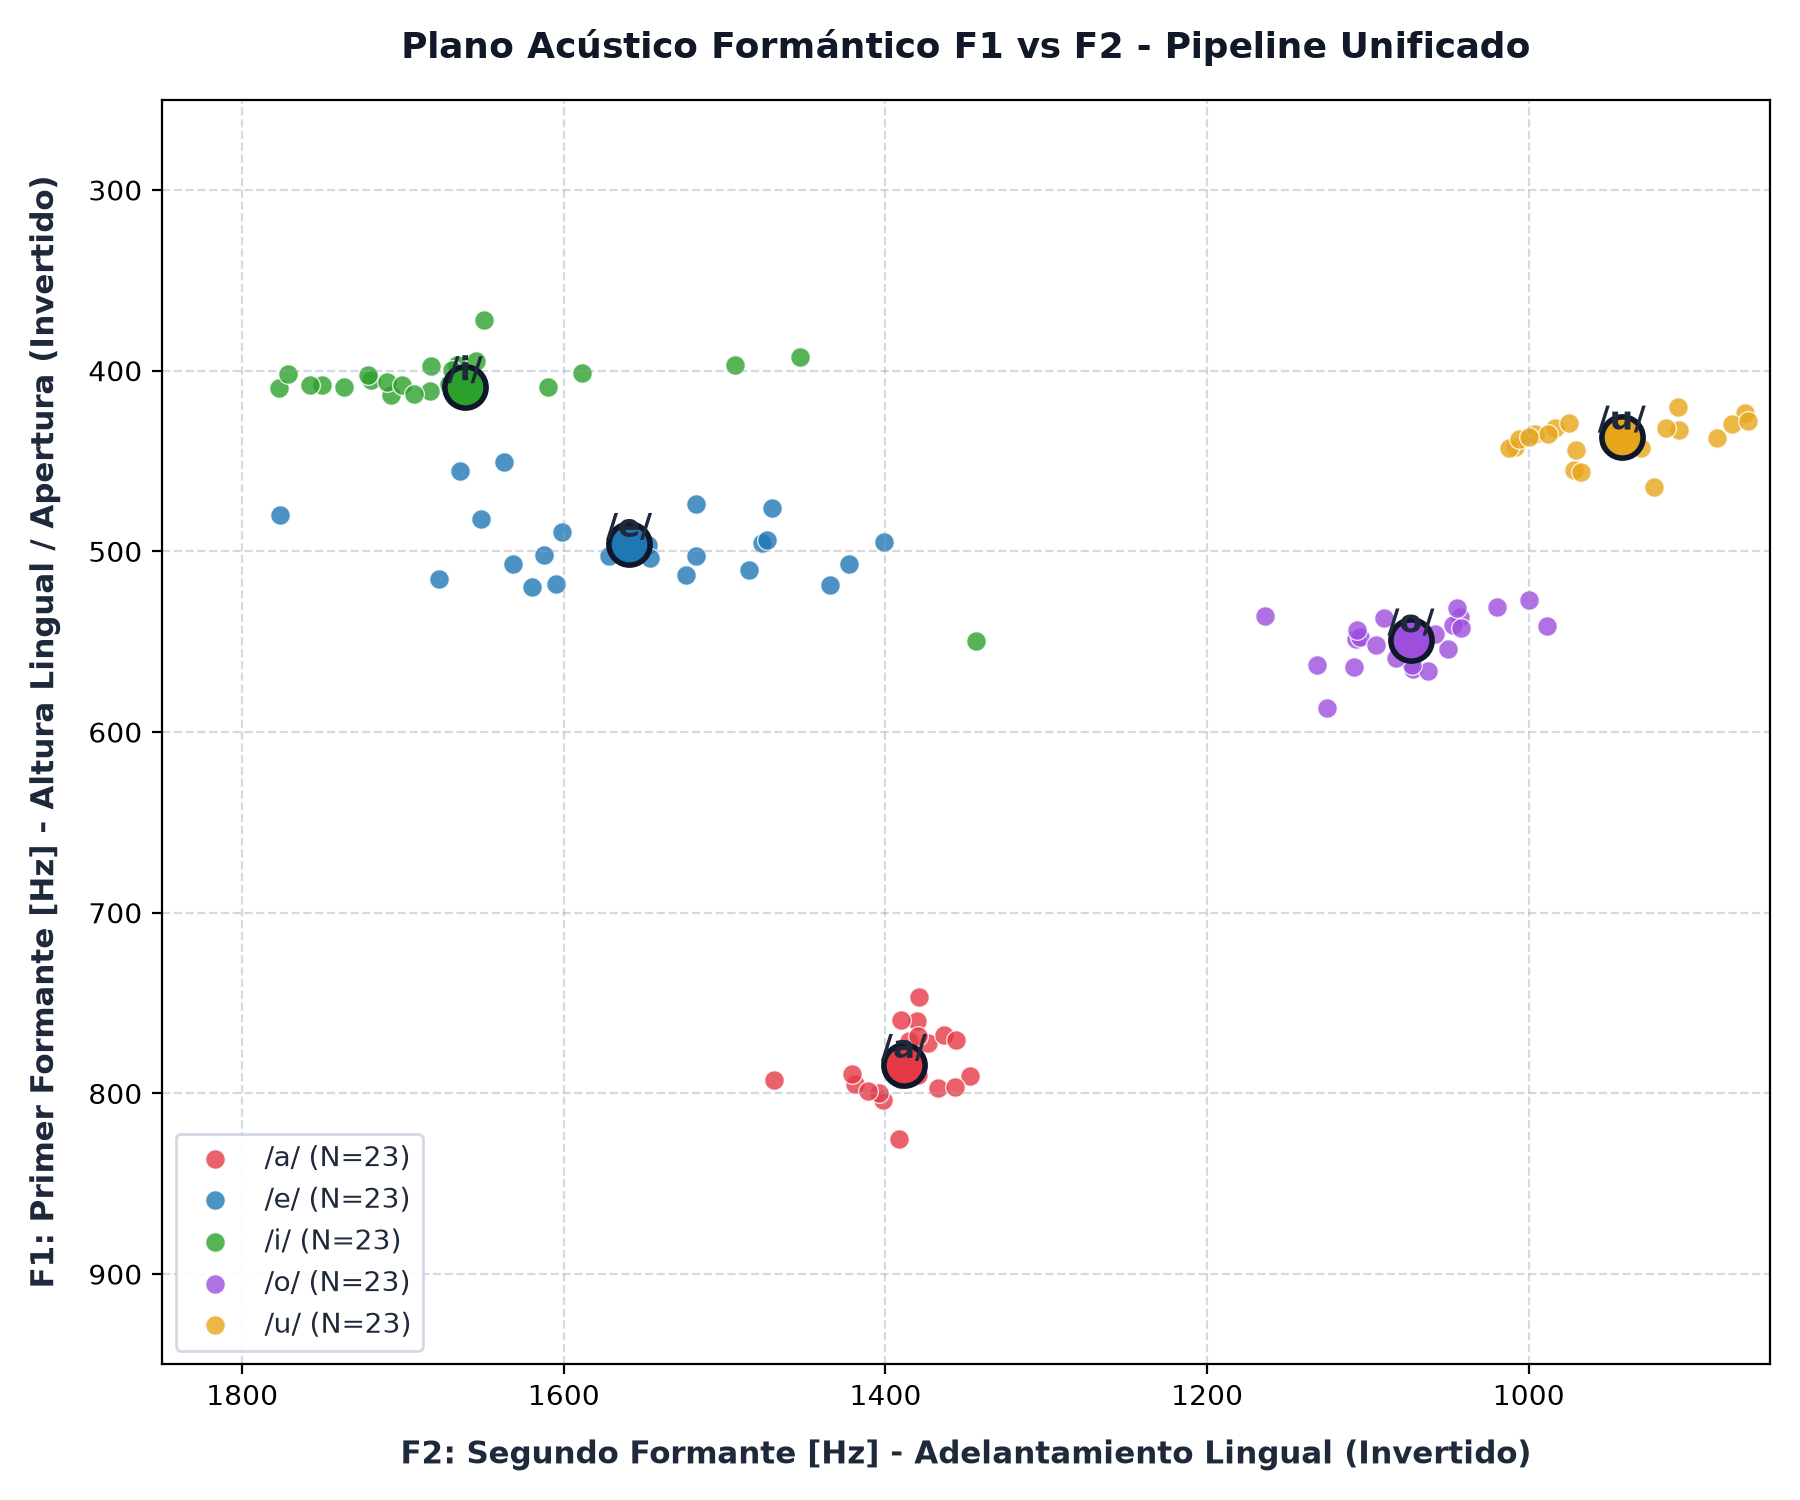
\includegraphics[width=\textwidth]{figuras/exp2/plano_formantes_lineal.png}
        \caption{Exp. 2: Cadencia Natural 30 BPM}
    \end{subfigure}
    \vskip\baselineskip
    \begin{subfigure}[b]{0.48\textwidth}
        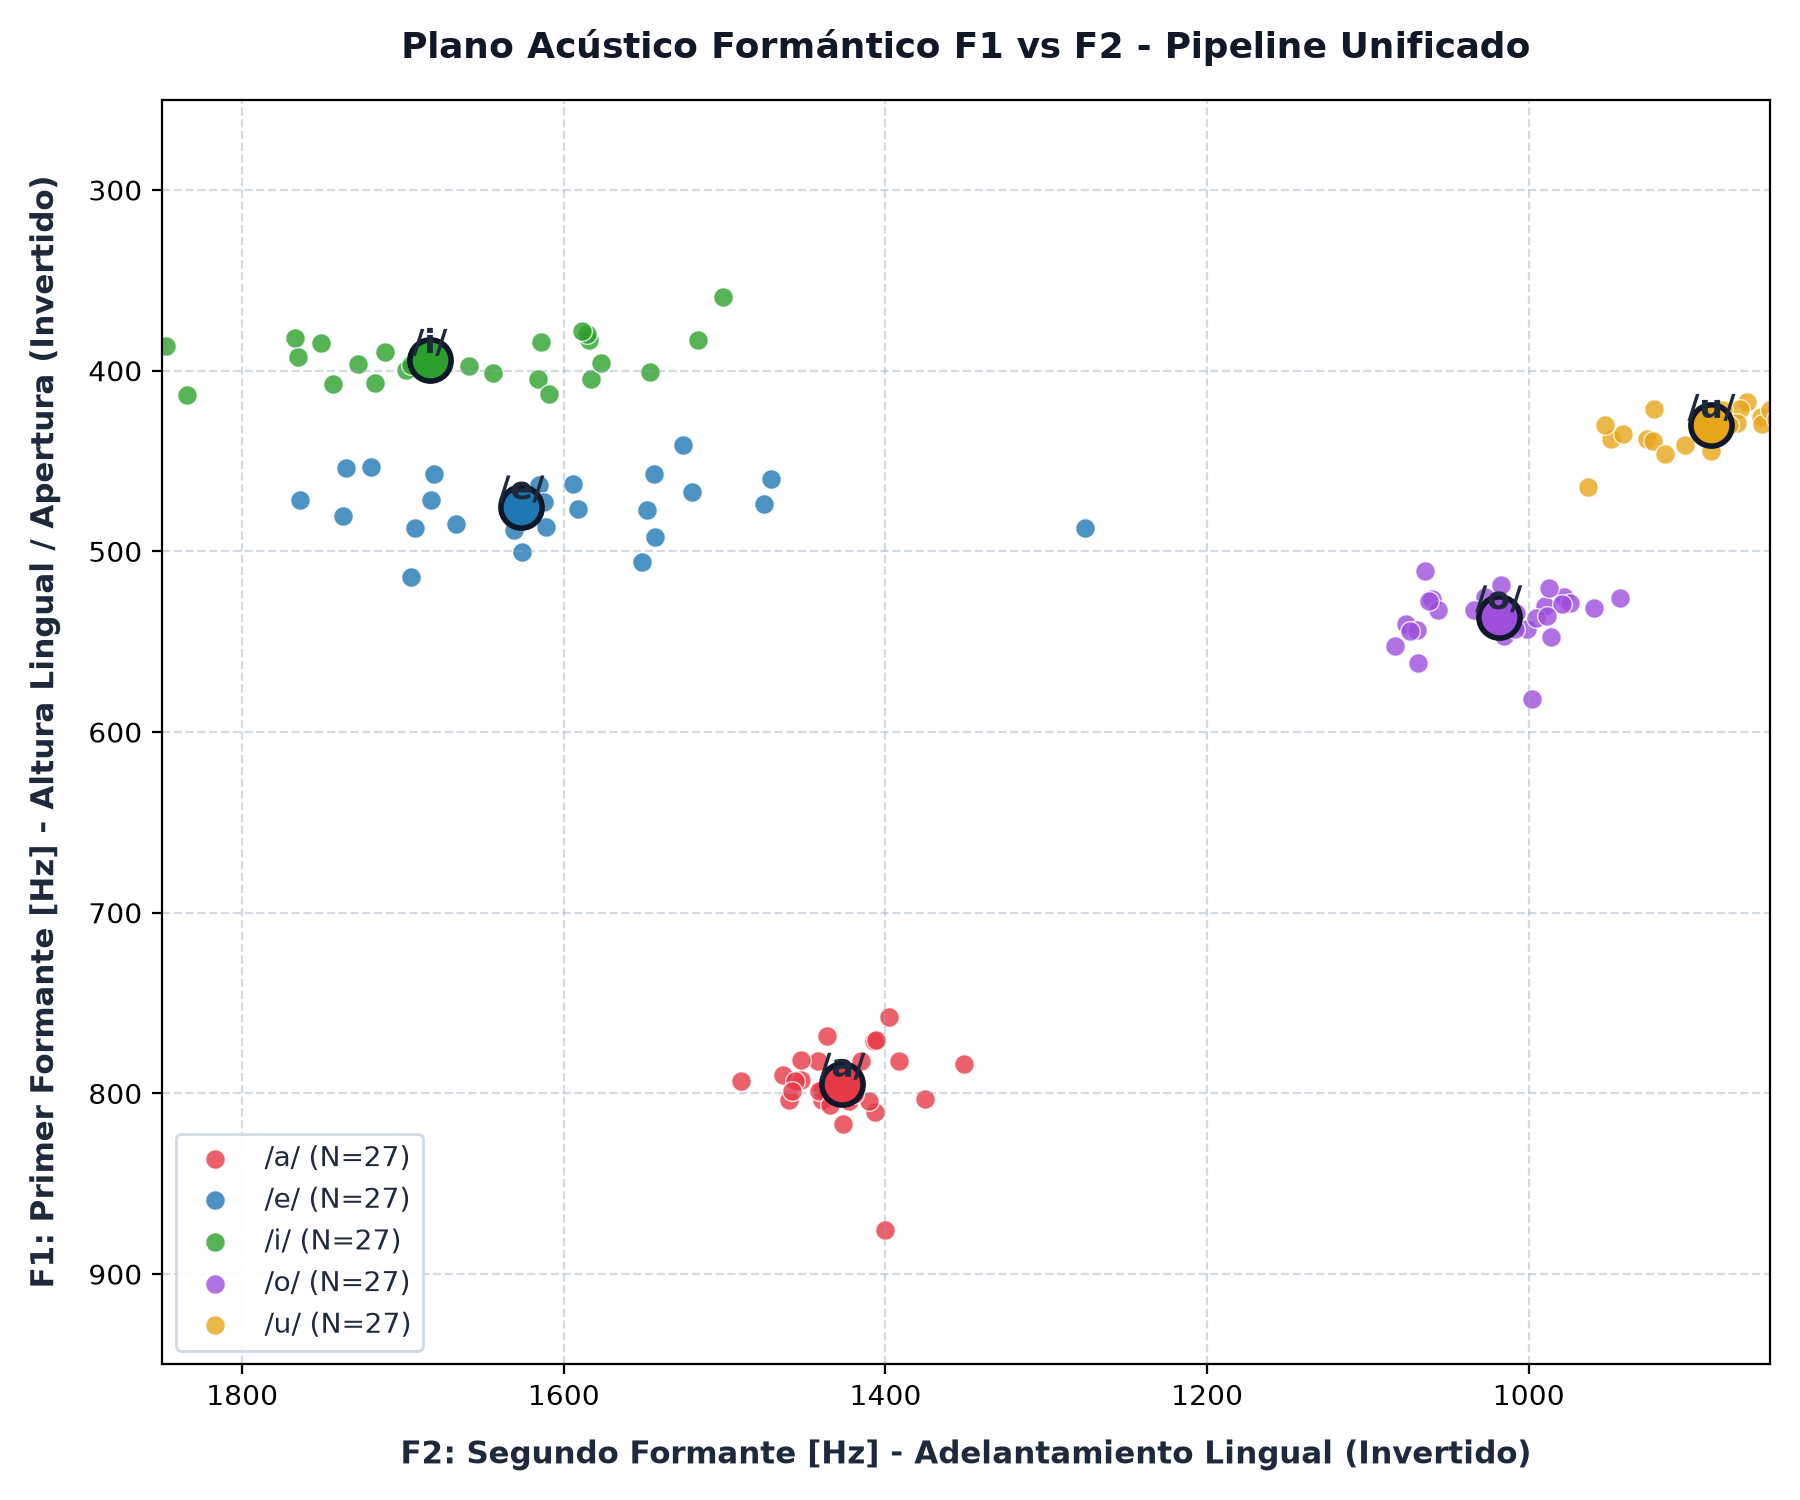
\includegraphics[width=\textwidth]{figuras/exp3/plano_formantes_lineal.png}
        \caption{Exp. 3: Cadencia Rápida 40 BPM}
    \end{subfigure}
    \hfill
    \begin{subfigure}[b]{0.48\textwidth}
        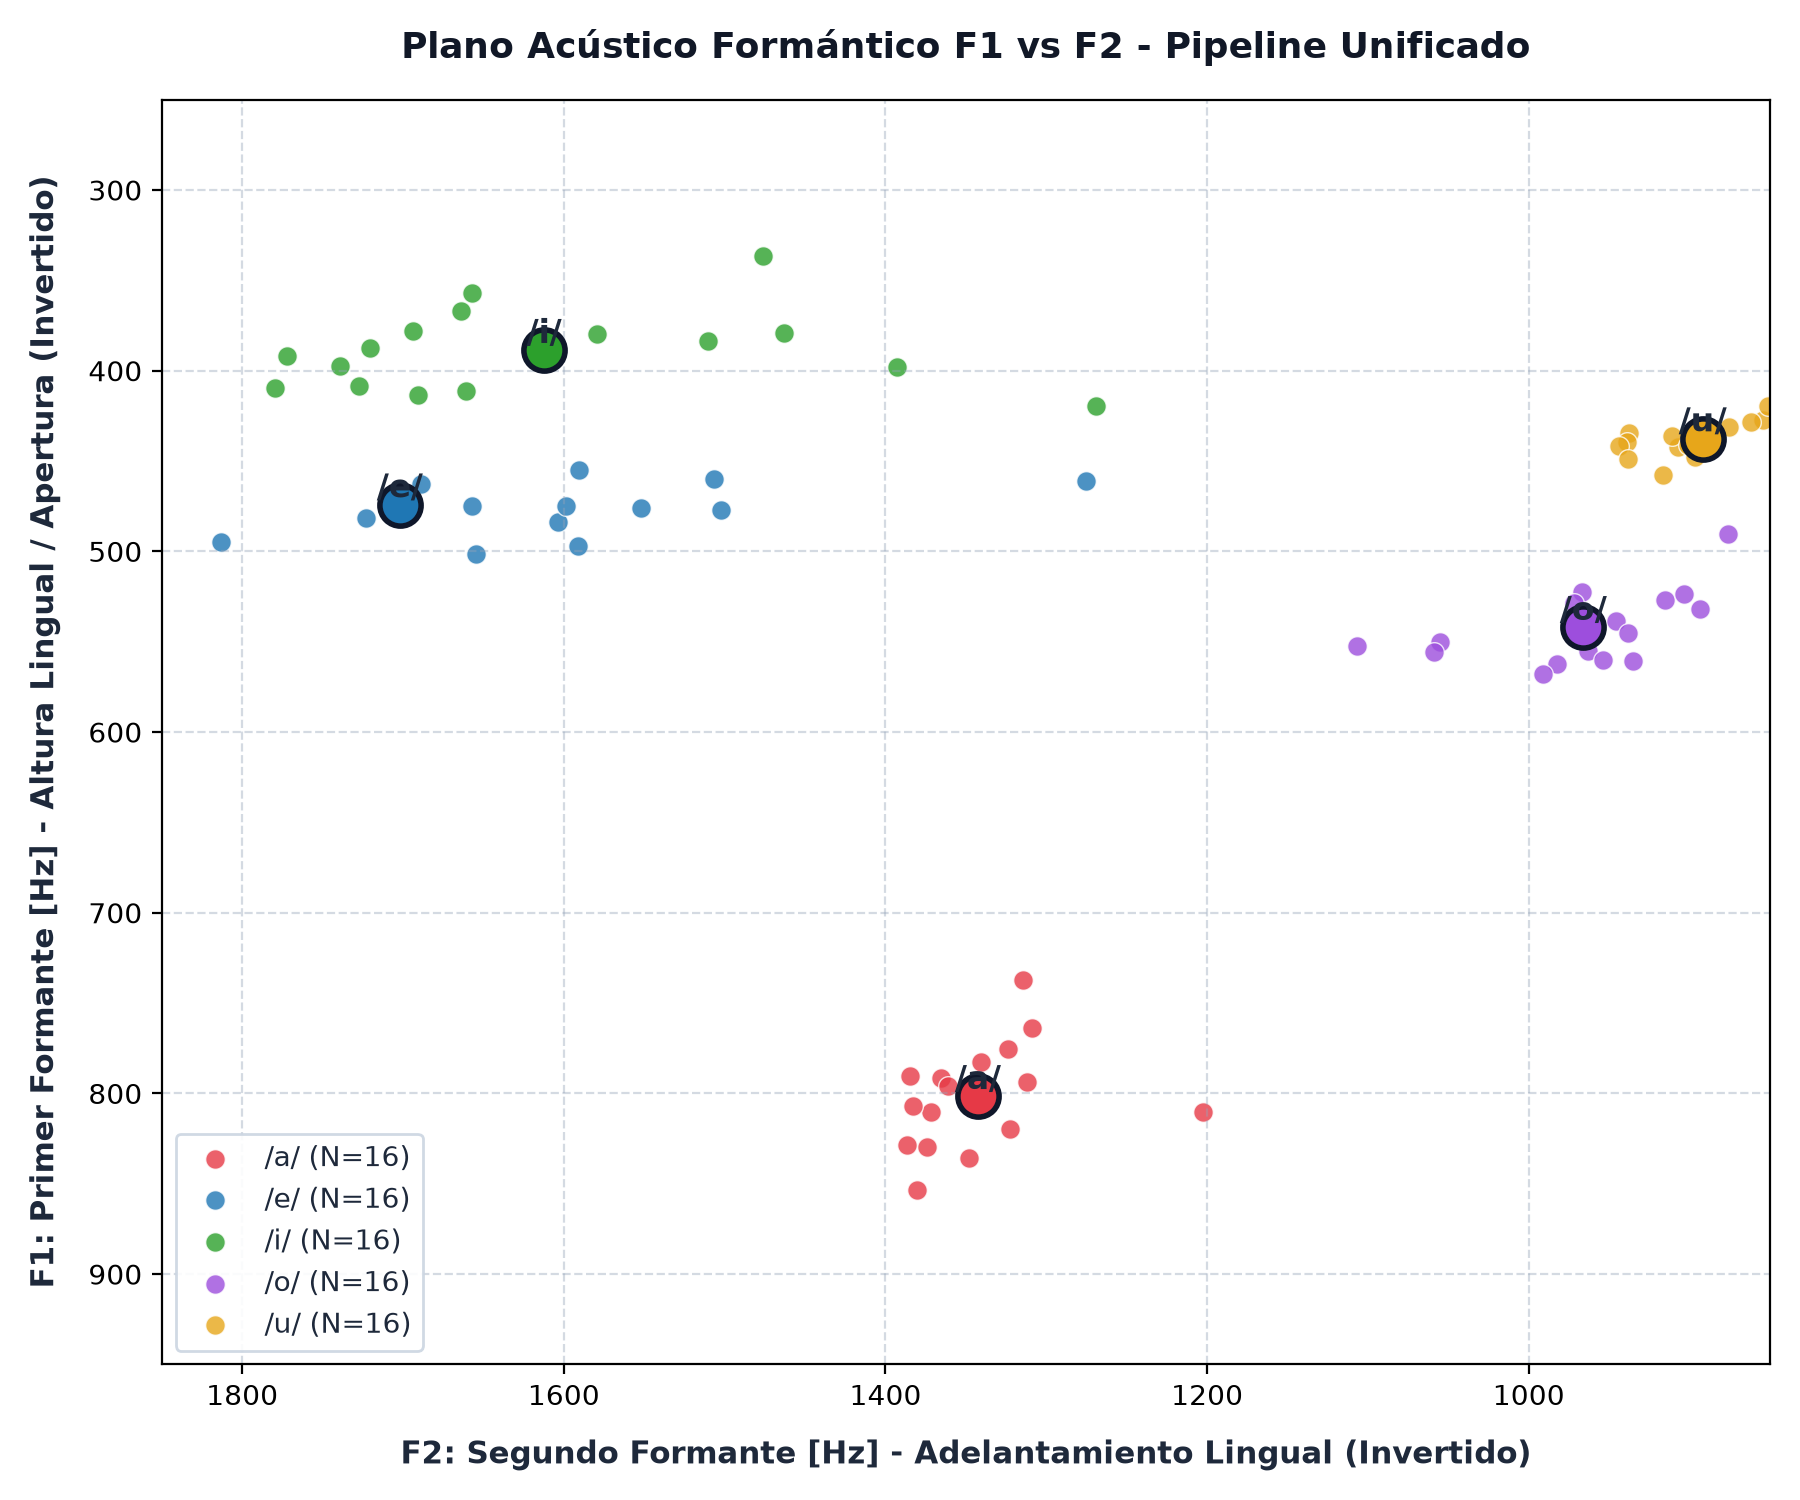
\includegraphics[width=\textwidth]{figuras/exp4/plano_formantes_lineal.png}
        \caption{Exp. 4: Invarianza Distancia / Pose}
    \end{subfigure}
    \caption{Planos formánticos convencionales $F_1$ vs $F_2$ para las cinco vocales fonéticas en los 4 experimentos.}
    \label{fig:planos_f1_f2}
\end{figure}

\newpage
\section{Topología Acústica Articulatoria: Planos F1 vs (F2 -- F1)}
Representación fonética desacoplada: el eje vertical ($F_1$) se asocia a la apertura bucal y descenso mandibular, mientras que el eje horizontal ($F_2 - F_1$) cuantifica el grado de anterioridad/adelantamiento lingual relativo.

\begin{figure}[htbp]
    \centering
    \begin{subfigure}[b]{0.48\textwidth}
        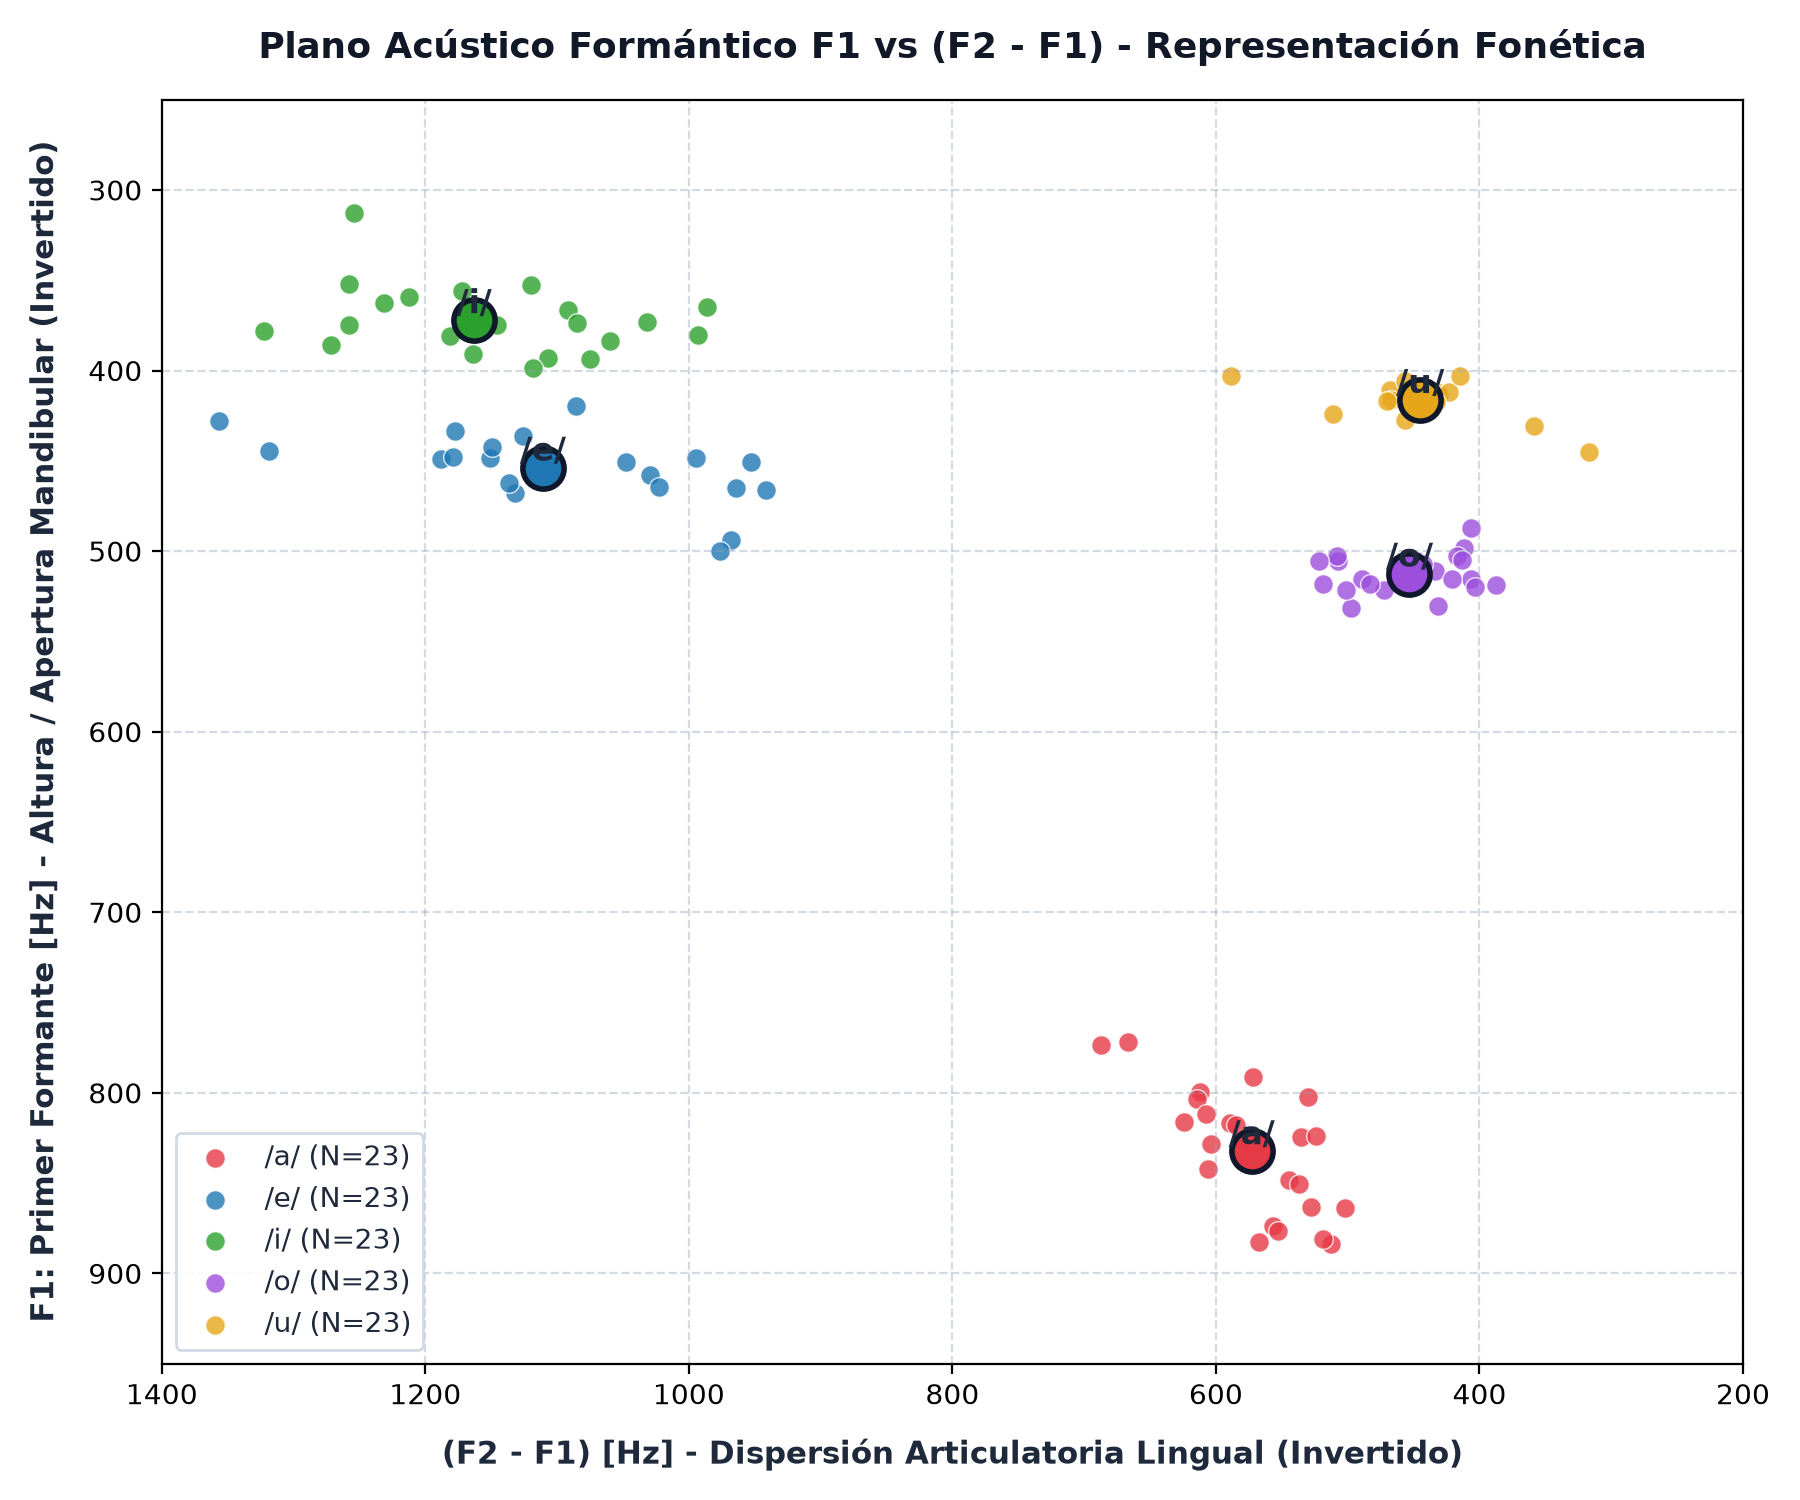
\includegraphics[width=\textwidth]{figuras/exp1/plano_formantes_f1_vs_diff.png}
        \caption{Exp. 1: Hiperarticulado 24 BPM}
    \end{subfigure}
    \hfill
    \begin{subfigure}[b]{0.48\textwidth}
        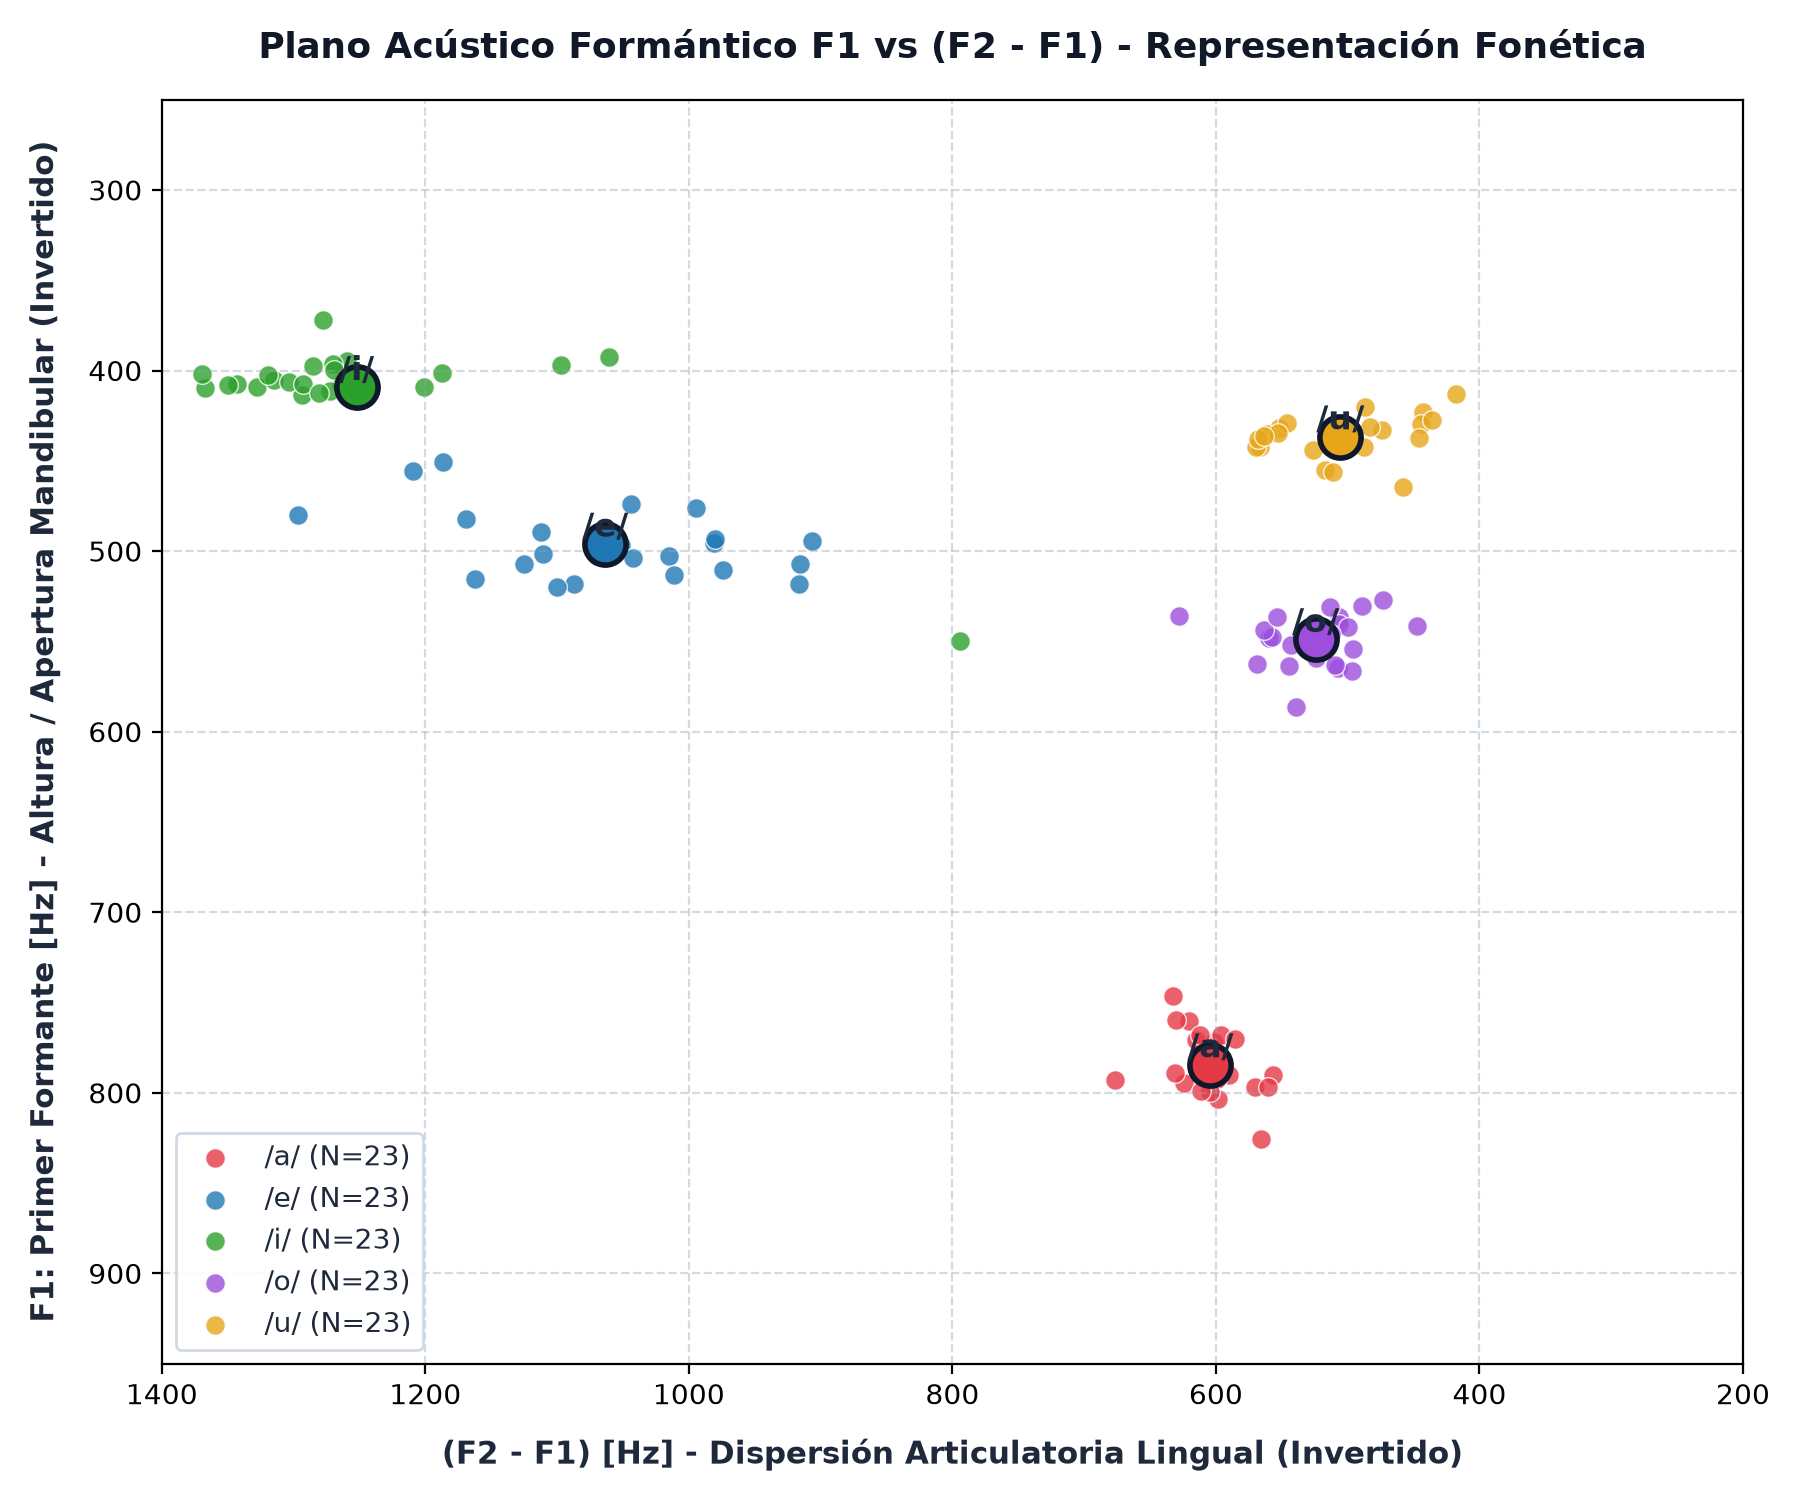
\includegraphics[width=\textwidth]{figuras/exp2/plano_formantes_f1_vs_diff.png}
        \caption{Exp. 2: Cadencia Natural 30 BPM}
    \end{subfigure}
    \vskip\baselineskip
    \begin{subfigure}[b]{0.48\textwidth}
        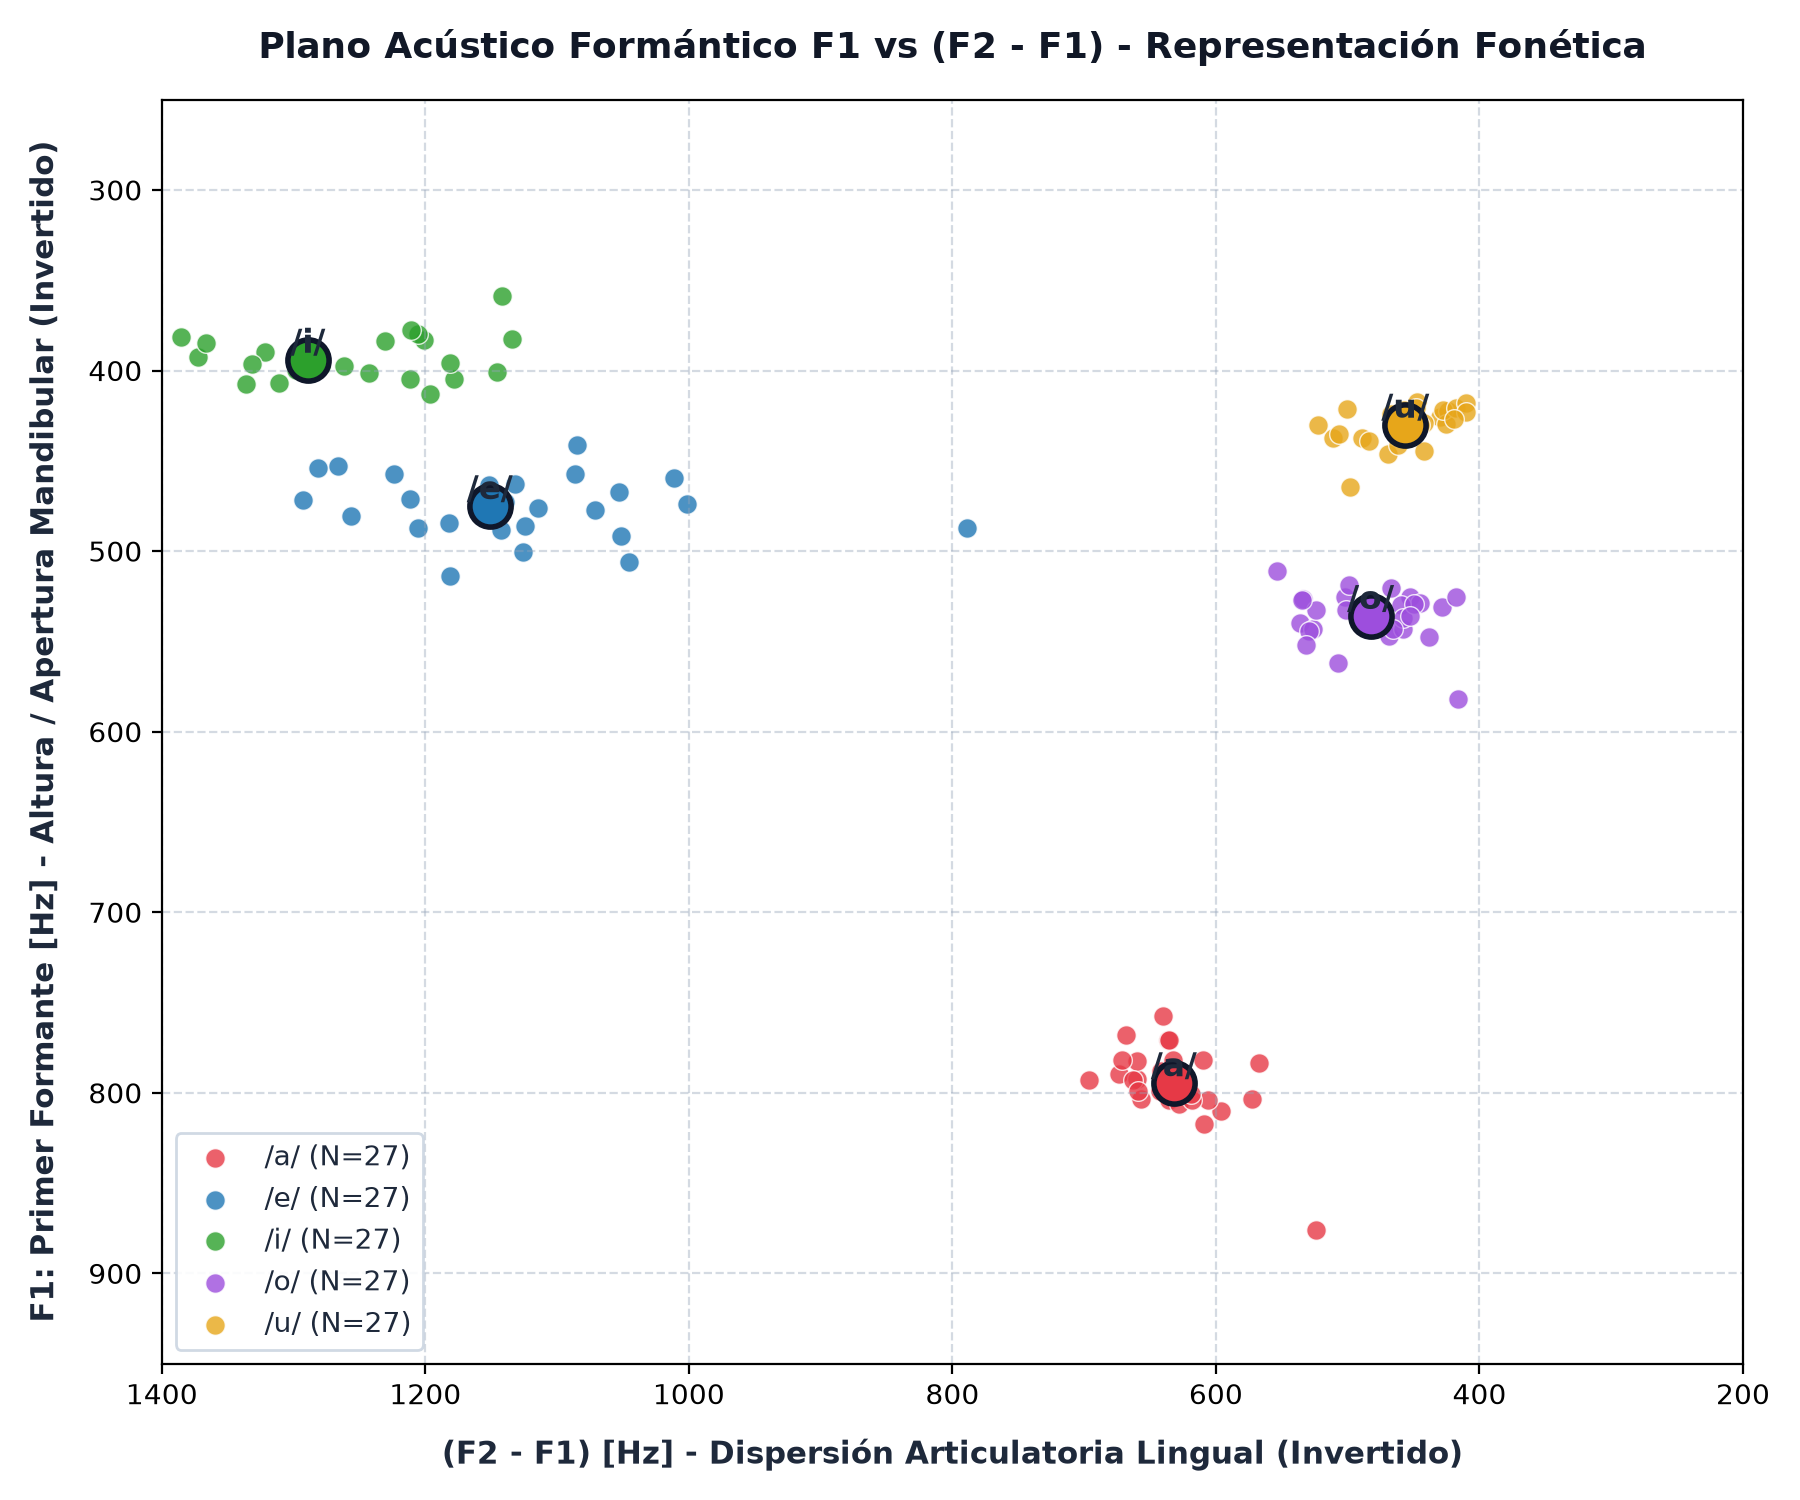
\includegraphics[width=\textwidth]{figuras/exp3/plano_formantes_f1_vs_diff.png}
        \caption{Exp. 3: Cadencia Rápida 40 BPM}
    \end{subfigure}
    \hfill
    \begin{subfigure}[b]{0.48\textwidth}
        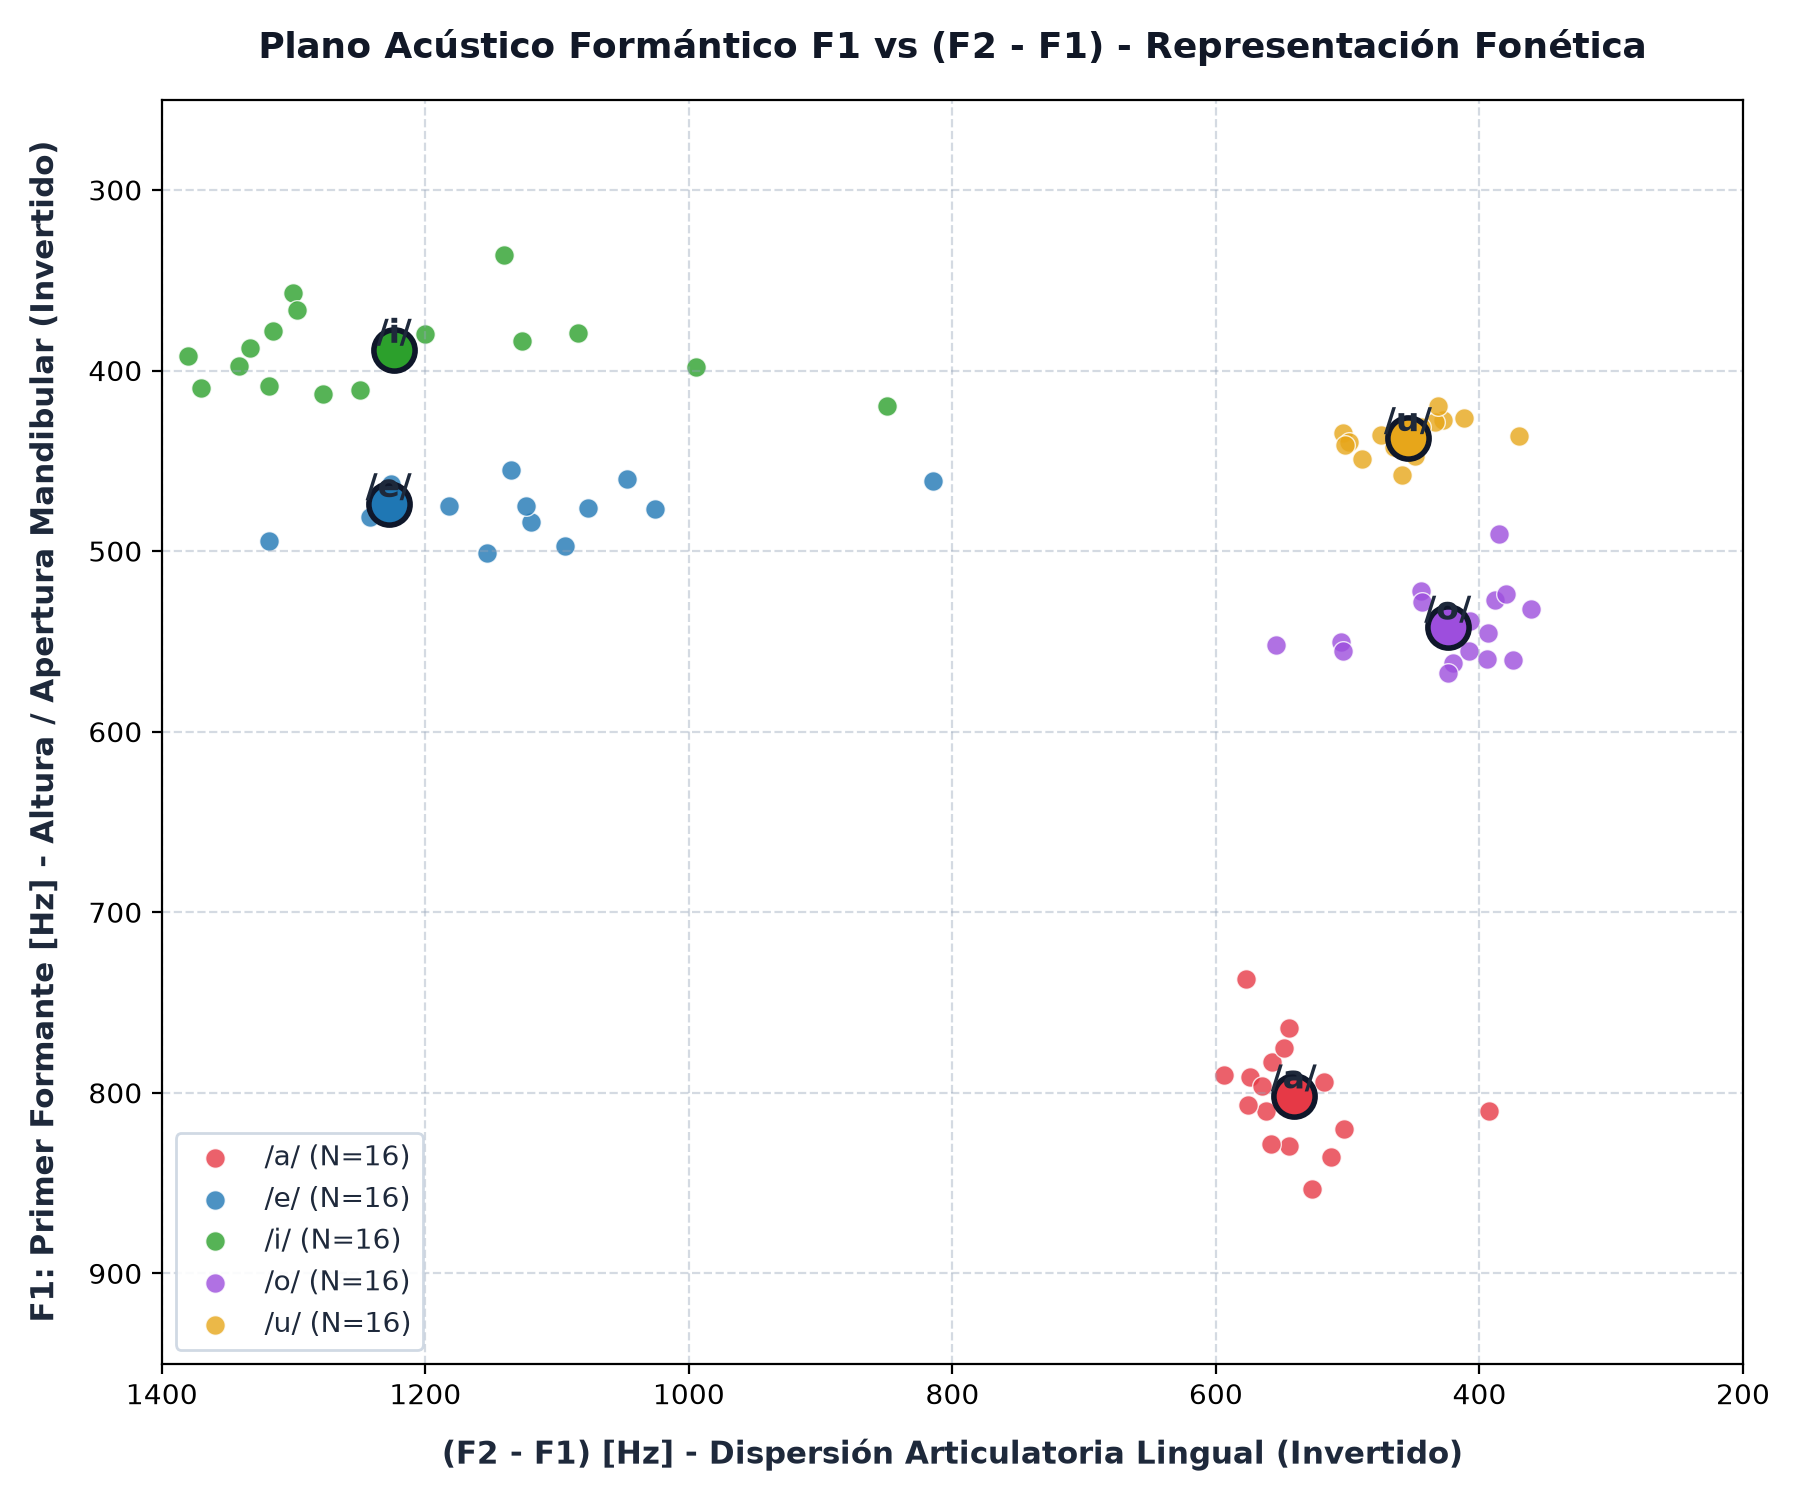
\includegraphics[width=\textwidth]{figuras/exp4/plano_formantes_f1_vs_diff.png}
        \caption{Exp. 4: Invarianza Distancia / Pose}
    \end{subfigure}
    \caption{Planos fonéticos articulatorios $F_1$ vs $(F_2 - F_1)$ en los 4 bloques evaluados.}
    \label{fig:planos_f1_diff}
\end{figure}

\newpage
\section{Discusión Comparativa y Conclusiones}
En la Tabla~\ref{tab:resumen_metrica} se resume el rendimiento de decodificación y estabilidad del espacio latente tridimensional a lo largo de las cuatro condiciones evaluadas.

\begin{table}[htbp]
    \centering
    \small
    \caption{Comparativa global de decodificación cinemática en espacio PCA 3D.}
    \label{tab:resumen_metrica}
    \begin{tabular}{lcccccc}
        \toprule
        \textbf{Experimento} & \textbf{Condición} & \textbf{BPM / Jitter} & \textbf{Pulsos $N$} & \textbf{Var. 3D (\%)} & \textbf{LDA Global (\%)} & \textbf{K-Means (\%)} \\
        \midrule
        Bloque 1 & Hiperarticulado & 24 BPM (De Bruijn) & 115 & 93.9 & \textbf{81.7} & 71.3 \\
        Bloque 2 & Cadencia Natural & 30 BPM (Jit 15\%) & 115 & 92.6 & \textbf{74.8} & 60.9 \\
        Bloque 3 & Cadencia Rápida & 40 BPM (Jit 20\%) & 135 & 84.8 & \textbf{65.9} & 53.3 \\
        Bloque 4 & Invarianza Pose & 24 BPM ($\Delta z, \Delta\theta$) & 80 & 92.4 & \textbf{80.0} & 70.0 \\
        \bottomrule
    \end{tabular}
\end{table}

\subsection{Evaluación Multidimensional: LDA en 4D y Variedades No Lineales Isomap}
Para analizar la capacidad intrínseca del espacio cinemático más allá de las primeras 3 componentes lineales, se evaluó la separabilidad lineal con un clasificador LDA sobre un espacio de dimensión 4 ($d=4$), comparando la formulación directa de 3 canales frente a la expansión de 6 canales. Asimismo, se proyectó el espacio de features sobre la variedad geodésica no lineal mediante \textbf{Isomap} utilizando el número óptimo de vecinos ($k=18$, determinado tras barrido sistemático) en subespacios de dimensión 2D, 3D y 4D:

\begin{table}[htbp]
    \centering
    \small
    \caption{Exactitud del clasificador lineal (LDA, \%) en PCA 4D y variedades geodésicas Isomap ($k=18$).}
    \label{tab:metricas_isomap_4d}
    \begin{tabular}{lcccccccc}
        \toprule
        & \multicolumn{4}{c}{\textbf{3 Canales Directos}} & \multicolumn{4}{c}{\textbf{6 Canales Bio-Inspirados}} \\
        \cmidrule(lr){2-5} \cmidrule(lr){6-9}
        \textbf{Experimento} & \textbf{PCA 4D} & \textbf{Iso 2D} & \textbf{Iso 3D} & \textbf{Iso 4D} & \textbf{PCA 4D} & \textbf{Iso 2D} & \textbf{Iso 3D} & \textbf{Iso 4D} \\
        \midrule
        Bloque 1 (24 BPM) & 79.1 & 80.0 & \textbf{80.9} & 80.0 & 78.3 & 78.3 & \textbf{80.0} & 75.7 \\
        Bloque 2 (30 BPM) & 74.8 & 74.8 & 73.0 & \textbf{76.5} & 70.4 & 72.2 & 72.2 & \textbf{72.2} \\
        Bloque 3 (40 BPM) & 65.9 & 55.6 & \textbf{60.0} & 58.5 & 63.7 & 57.8 & 57.8 & \textbf{60.7} \\
        Bloque 4 (Invar.) & 85.0 & 73.8 & 73.8 & \textbf{83.8} & 85.0 & 77.5 & 80.0 & \textbf{87.5} \\
        \bottomrule
    \end{tabular}
\end{table}

\subsection{Espacios Latentes Lineales: PCA 3D con Proyecciones Ortogonales}
En las figuras siguientes se ilustran las tres proyecciones ortogonales bidimensionales (PC1 vs PC2, PC1 vs PC3 y PC2 vs PC3) del espacio latente PCA 3D para cada uno de los 4 bloques experimentales. Se presentan tanto la formulación directa de 3 canales cinemáticos como la expansión bio-inspirada de 6 canales.

\subsubsection{PCA 3D - 3 Canales Directos}
\begin{figure}[htbp]
    \centering
    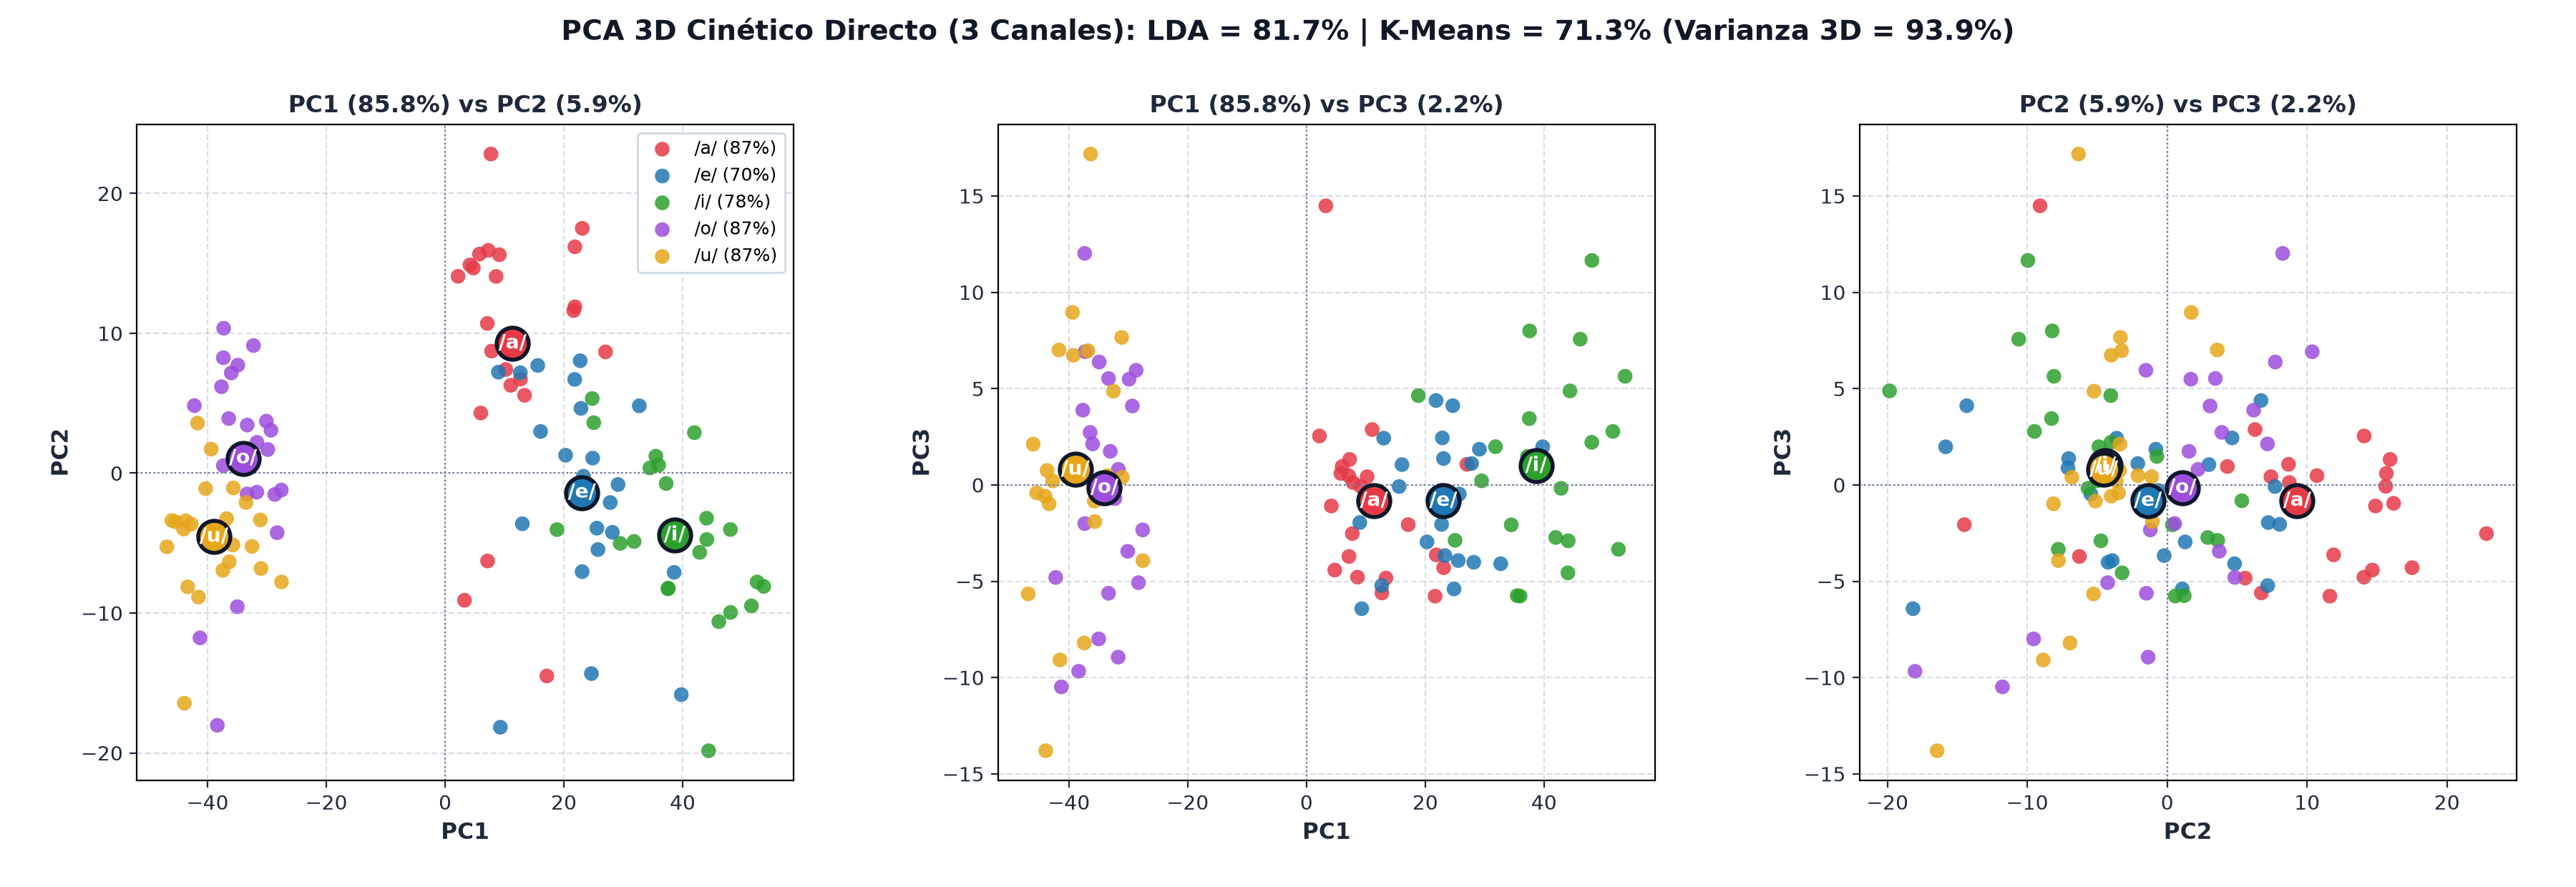
\includegraphics[width=\textwidth]{figuras/exp1/pca_cinetico_oficial.png}
    \caption{Espacio PCA 3D (3 canales directos) - Bloque 1: Hiperarticulado 24 BPM.}
    \label{fig:pca3d_3ch_exp1}
\end{figure}

\begin{figure}[htbp]
    \centering
    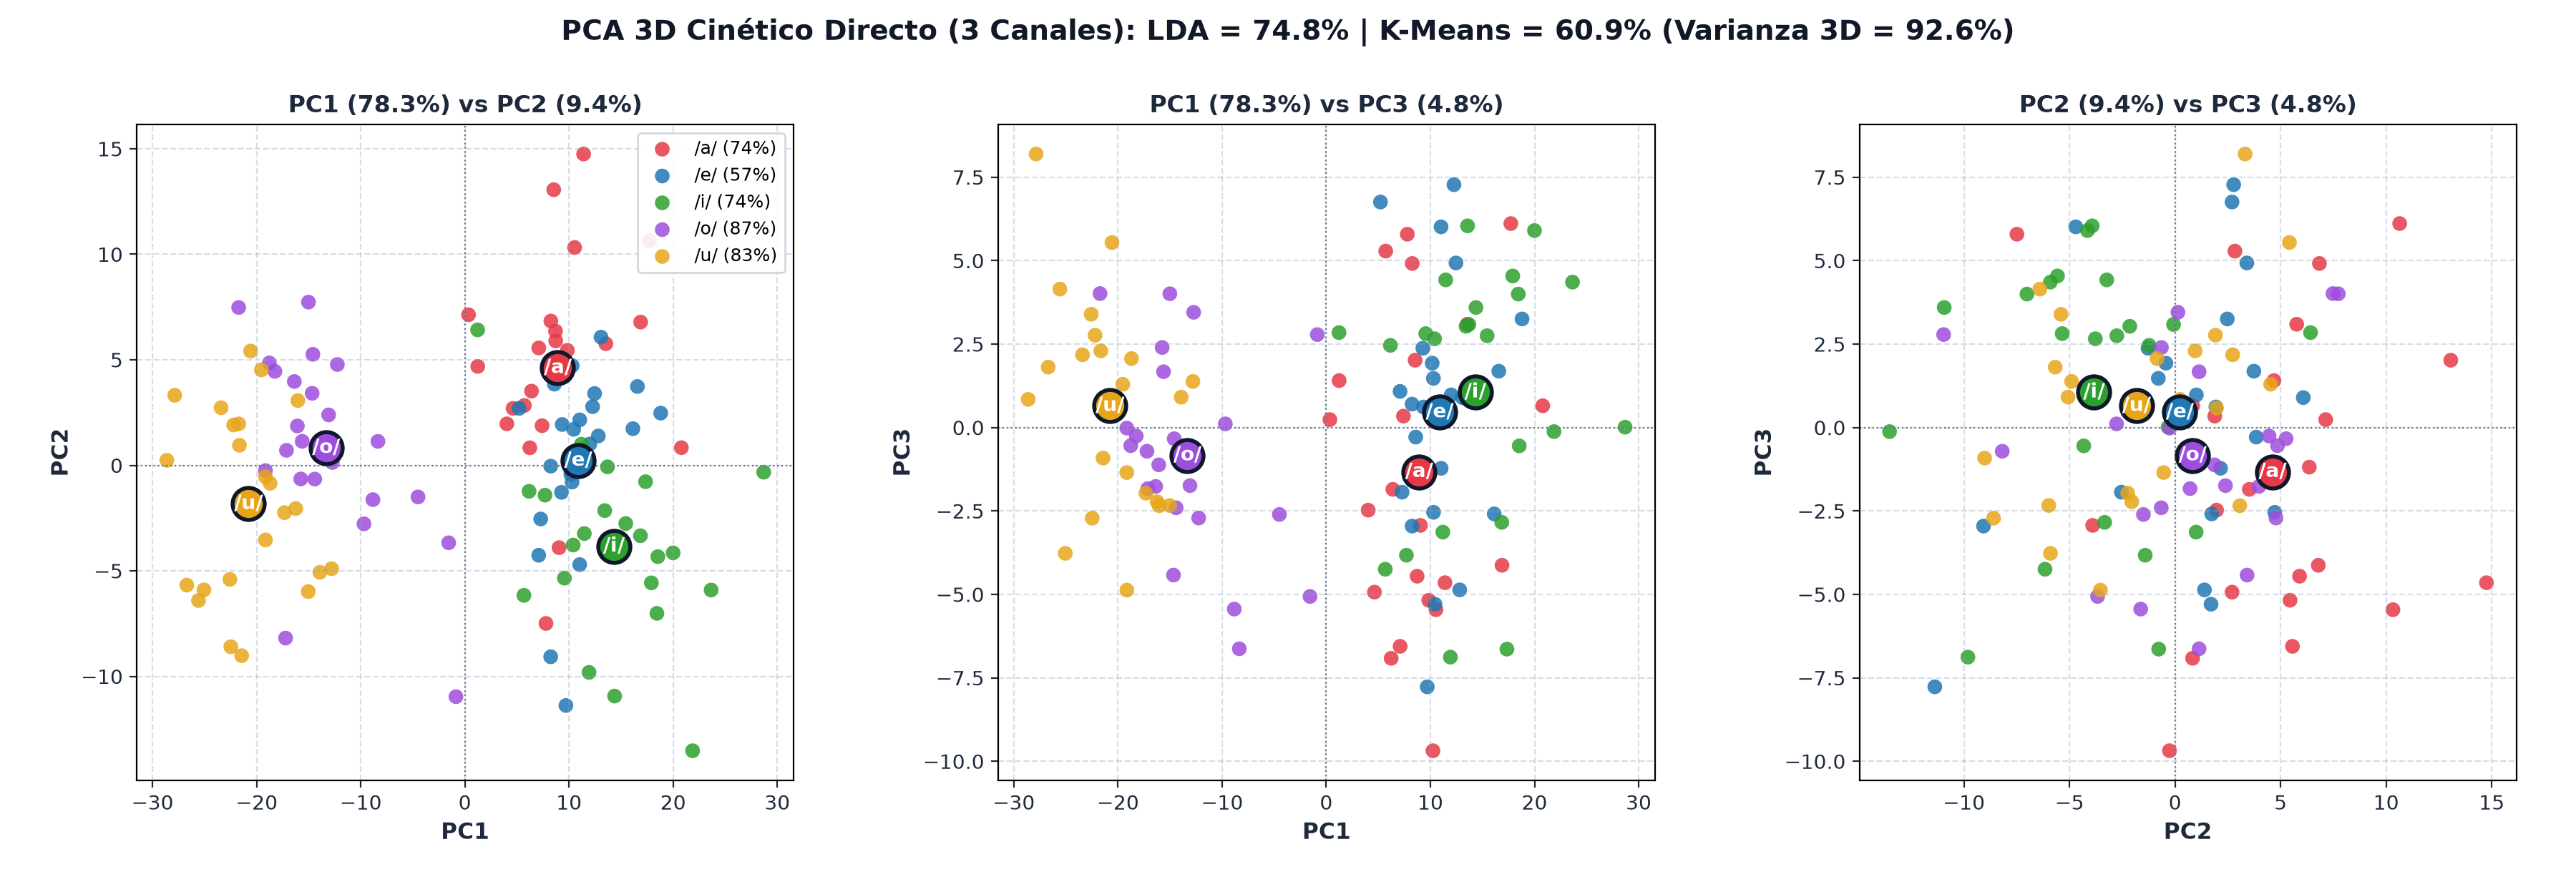
\includegraphics[width=\textwidth]{figuras/exp2/pca_cinetico_oficial.png}
    \caption{Espacio PCA 3D (3 canales directos) - Bloque 2: Cadencia Natural 30 BPM Jitter 15\%.}
    \label{fig:pca3d_3ch_exp2}
\end{figure}

\begin{figure}[htbp]
    \centering
    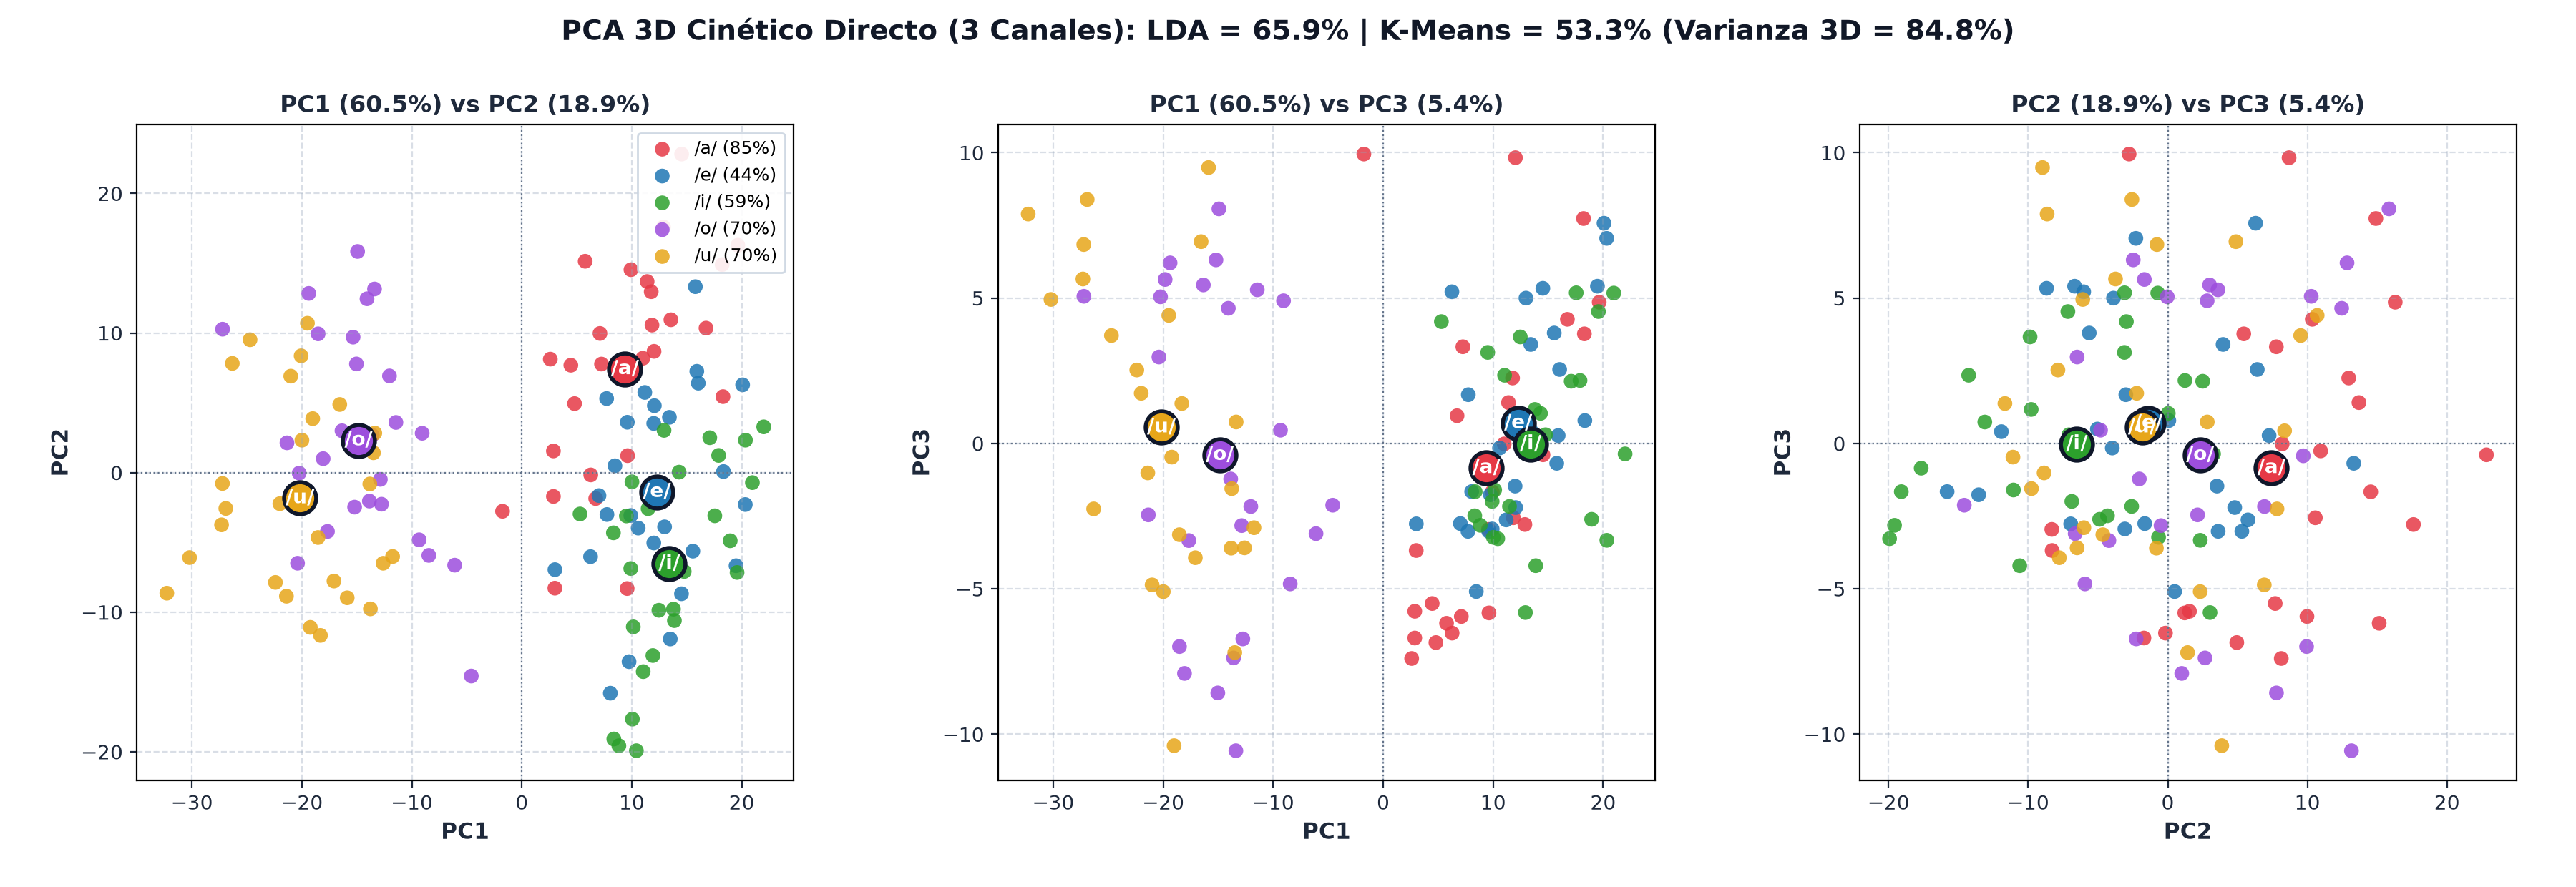
\includegraphics[width=\textwidth]{figuras/exp3/pca_cinetico_oficial.png}
    \caption{Espacio PCA 3D (3 canales directos) - Bloque 3: Cadencia Rápida 40 BPM Jitter 20\%.}
    \label{fig:pca3d_3ch_exp3}
\end{figure}

\begin{figure}[htbp]
    \centering
    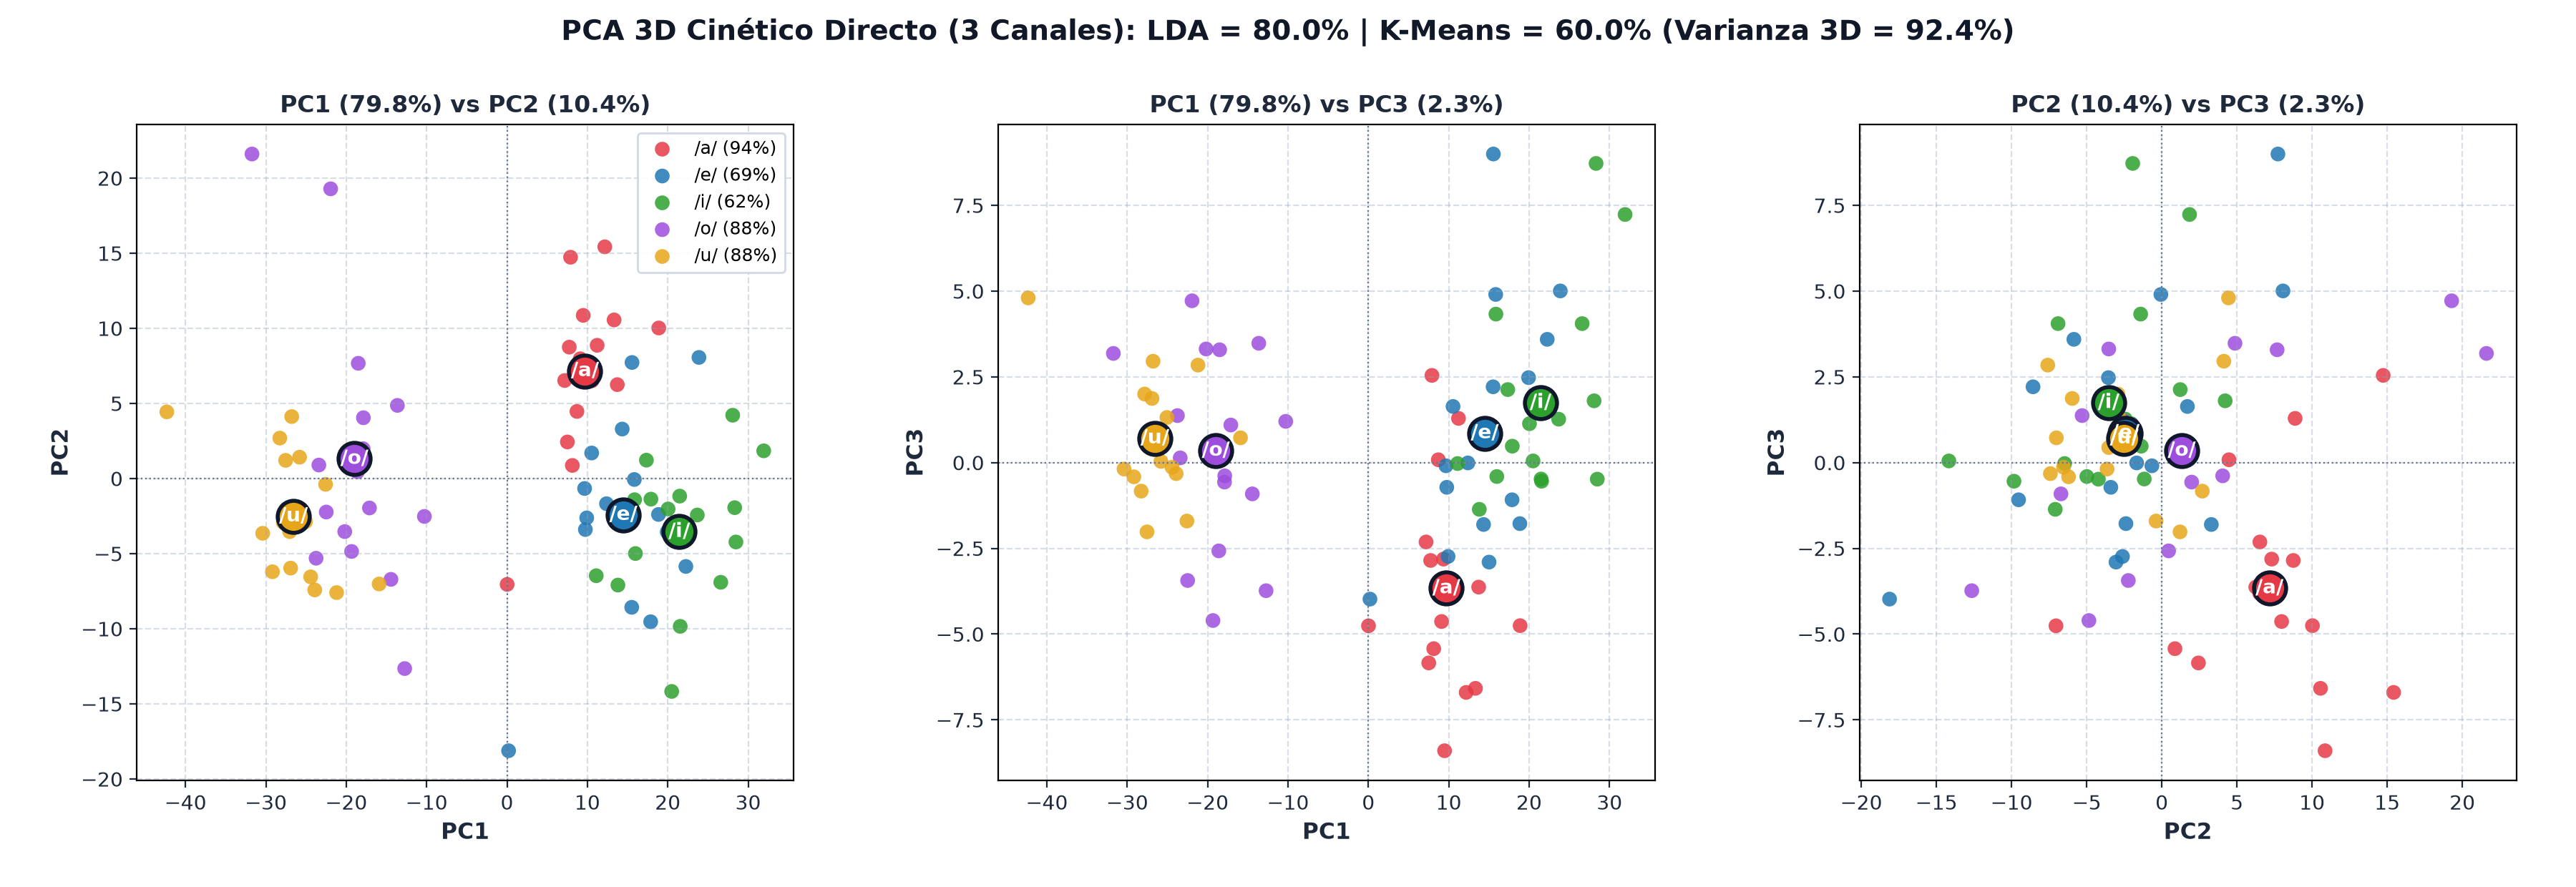
\includegraphics[width=\textwidth]{figuras/exp4/pca_cinetico_oficial.png}
    \caption{Espacio PCA 3D (3 canales directos) - Bloque 4: Invarianza a Distancia Focal y Rotación de Pose.}
    \label{fig:pca3d_3ch_exp4}
\end{figure}

\clearpage
\subsubsection{PCA 3D - 6 Canales Bio-Inspirados}
\begin{figure}[htbp]
    \centering
    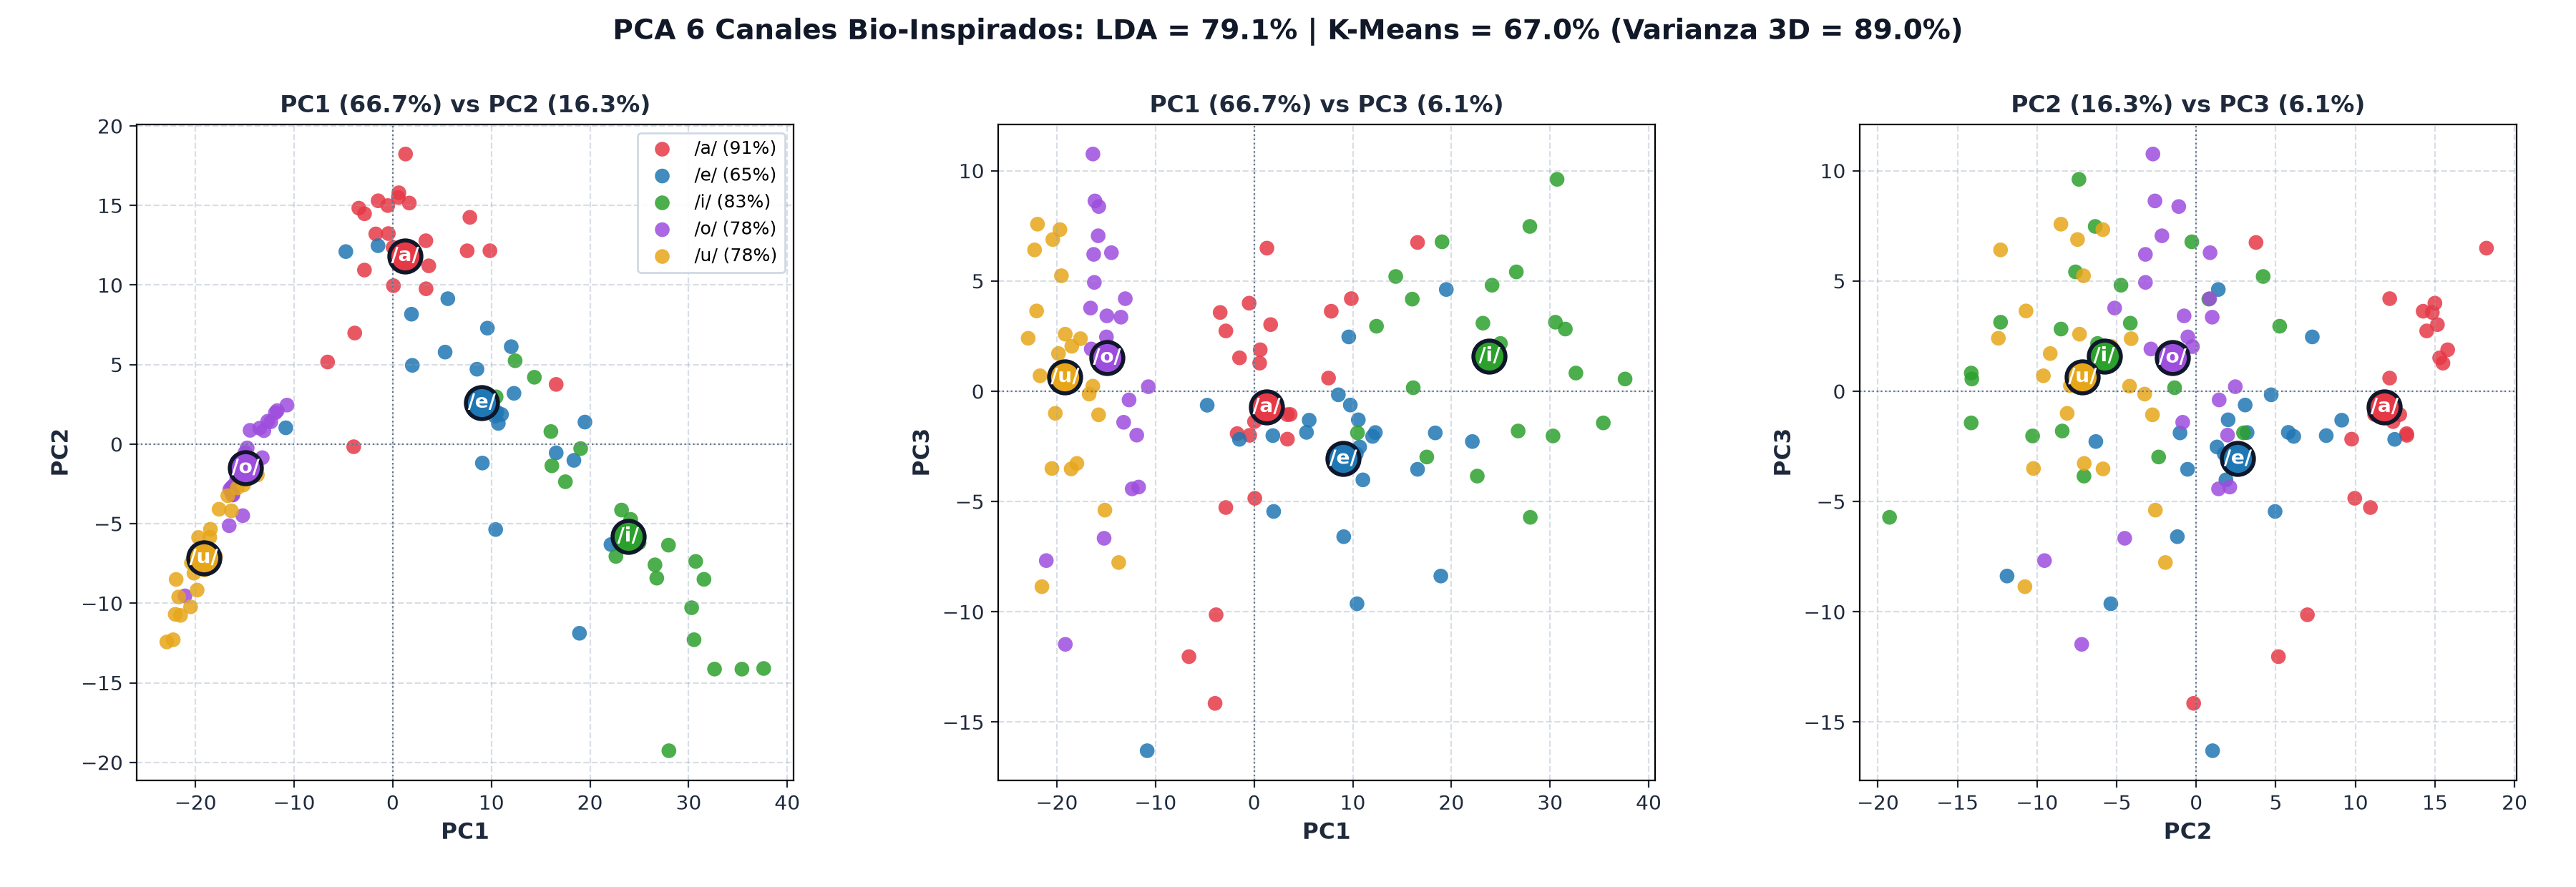
\includegraphics[width=\textwidth]{figuras/exp1/pca_6canales_oficial.png}
    \caption{Espacio PCA 3D (6 canales bio-inspirados) - Bloque 1: Hiperarticulado 24 BPM.}
    \label{fig:pca3d_6ch_exp1}
\end{figure}

\begin{figure}[htbp]
    \centering
    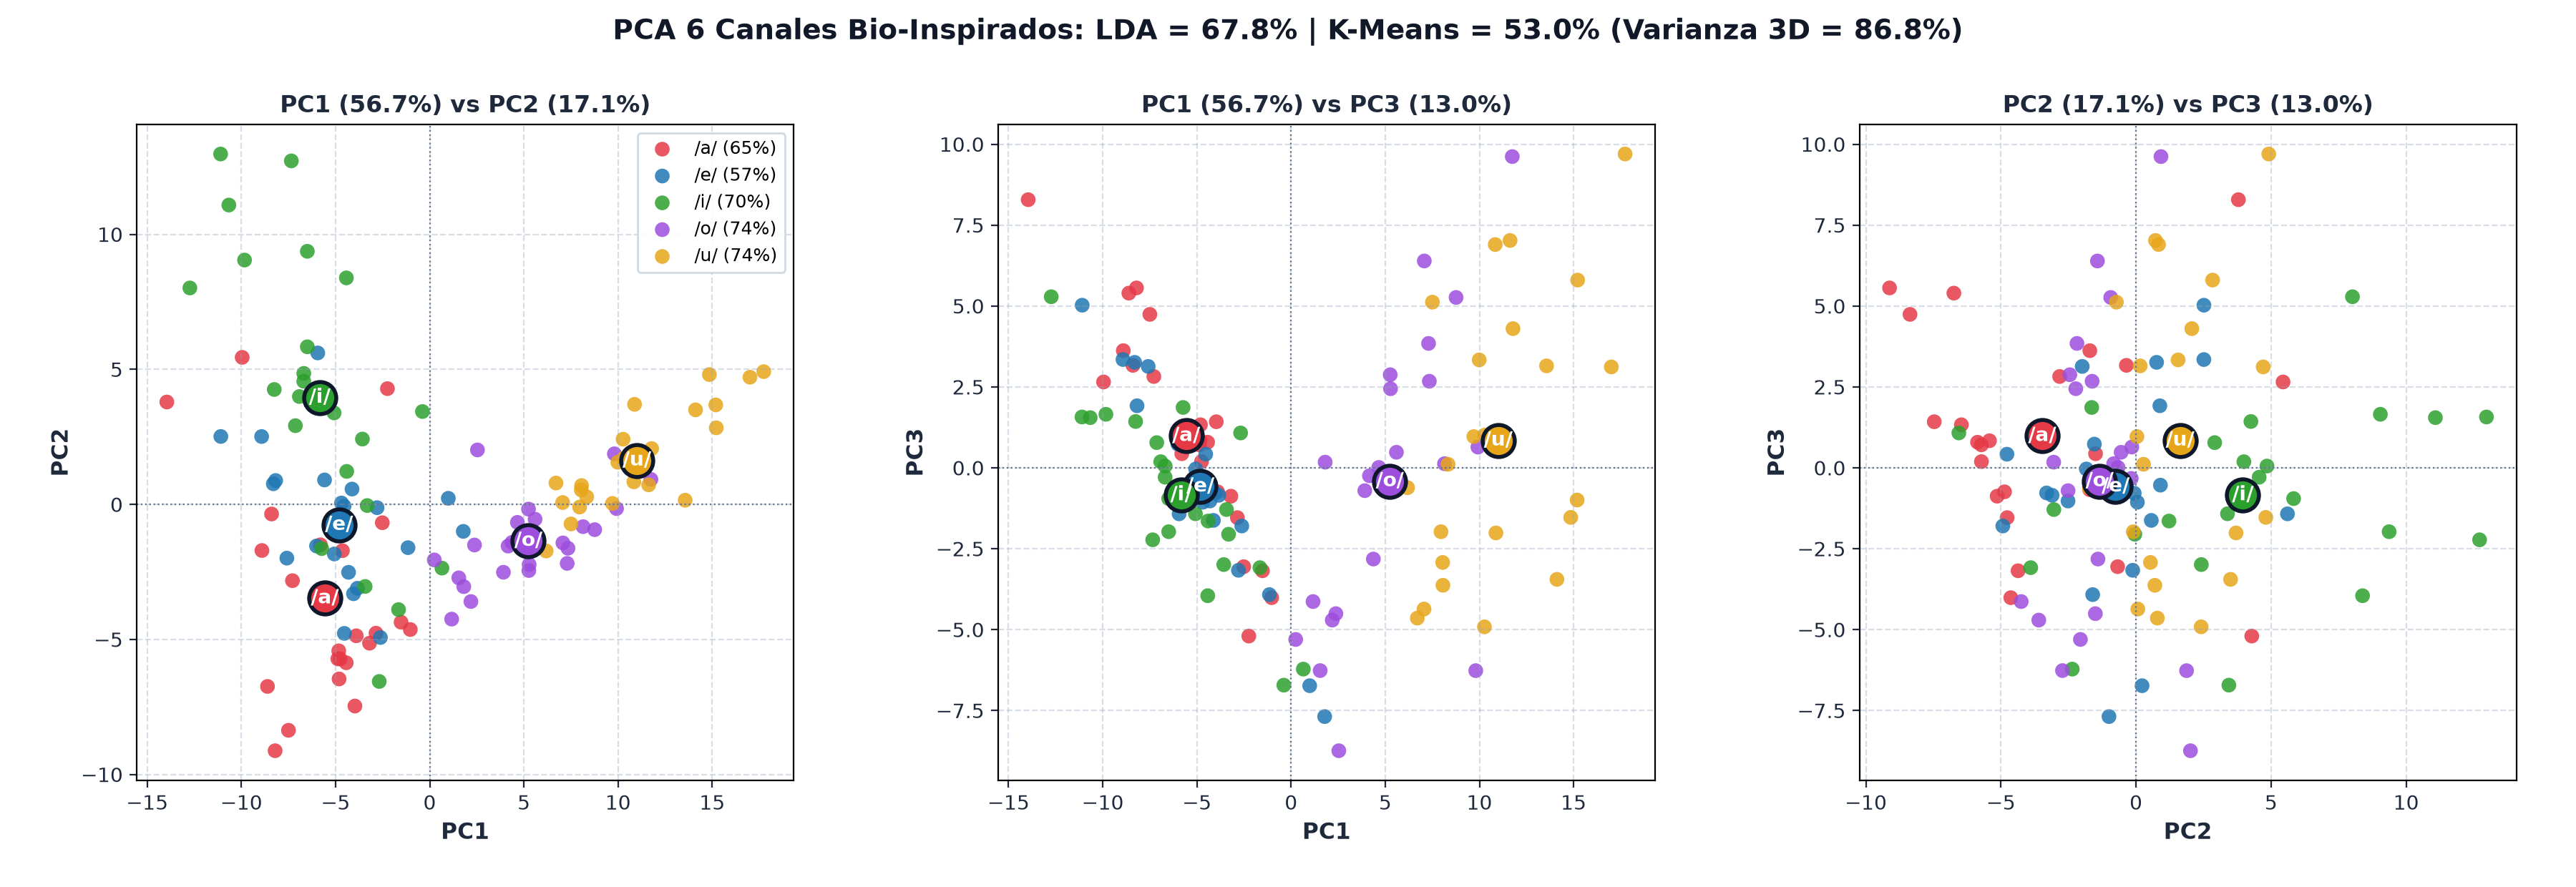
\includegraphics[width=\textwidth]{figuras/exp2/pca_6canales_oficial.png}
    \caption{Espacio PCA 3D (6 canales bio-inspirados) - Bloque 2: Cadencia Natural 30 BPM Jitter 15\%.}
    \label{fig:pca3d_6ch_exp2}
\end{figure}

\begin{figure}[htbp]
    \centering
    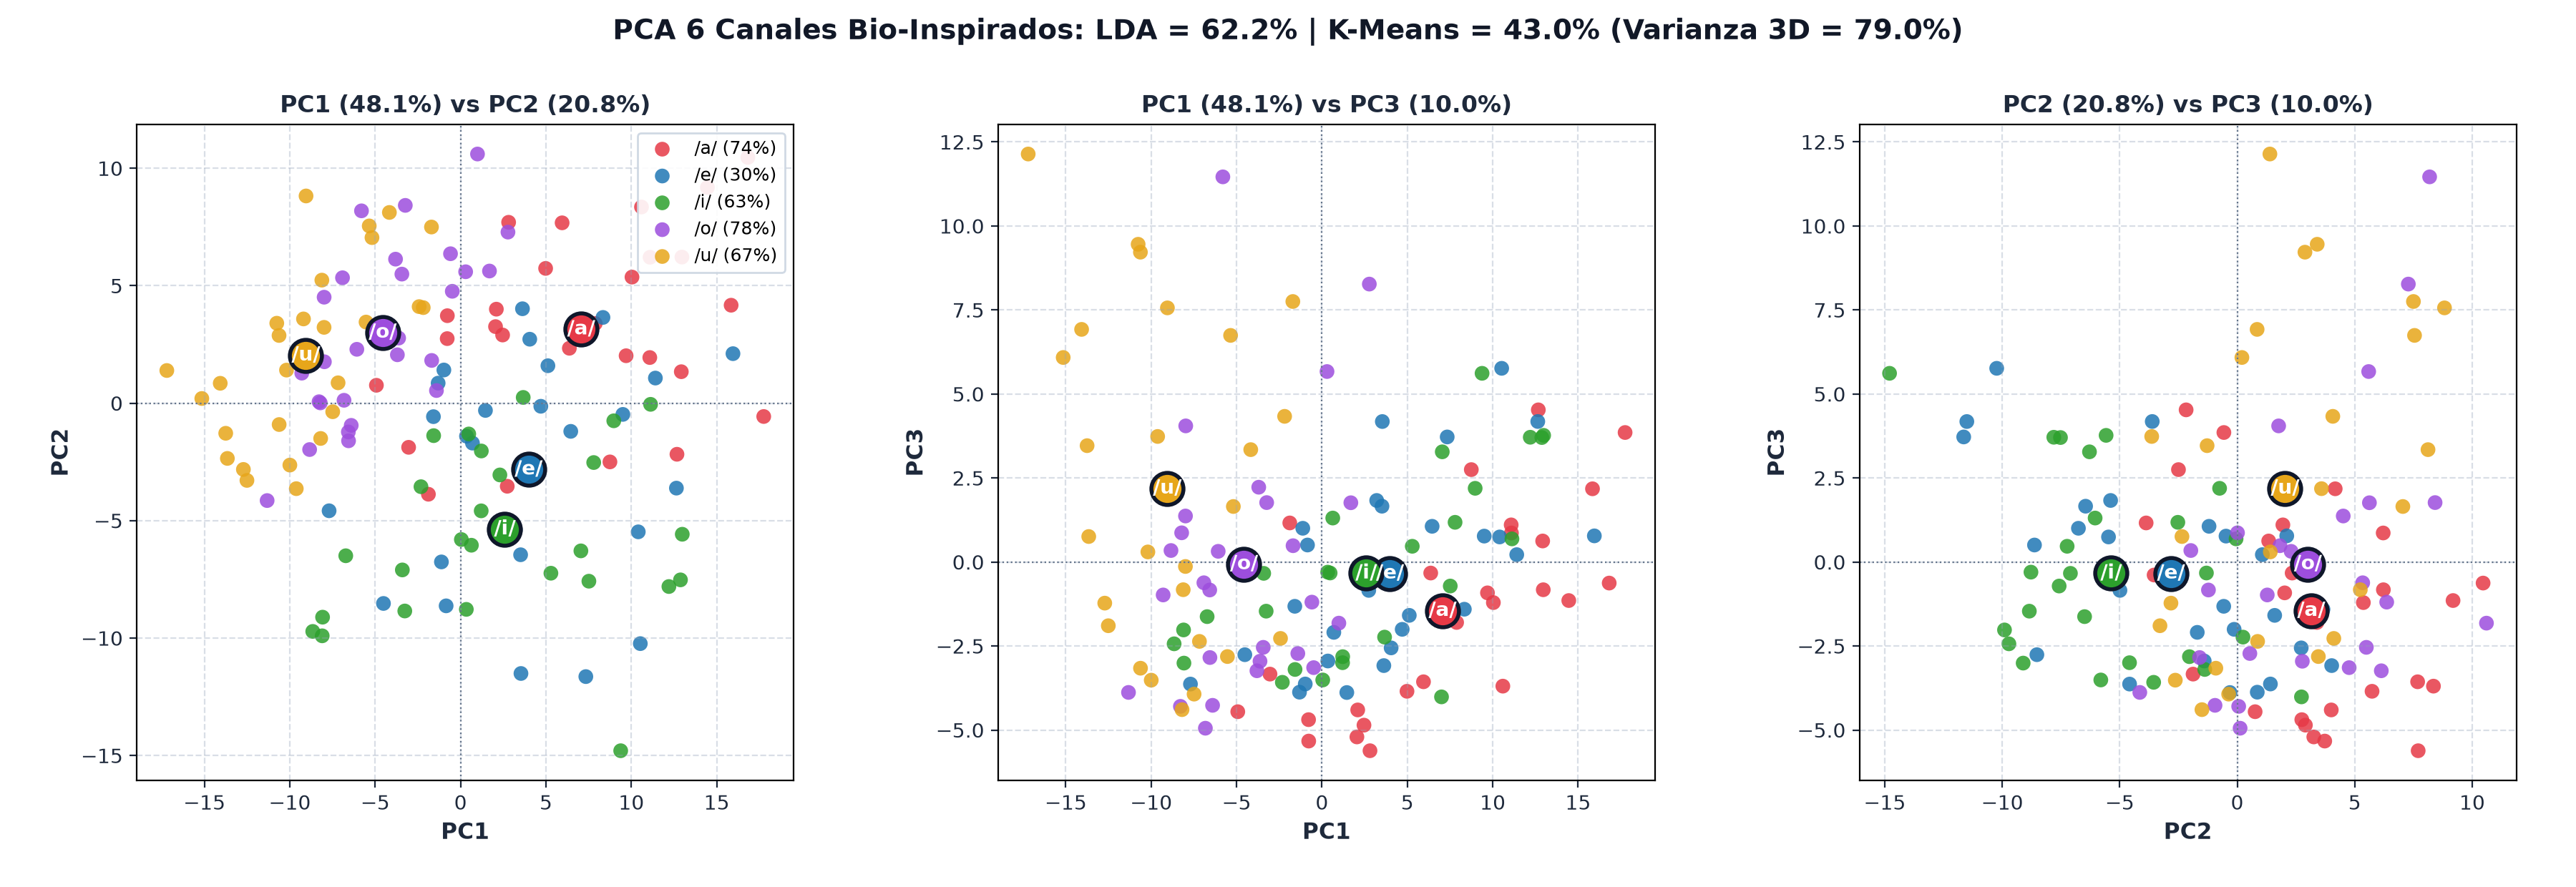
\includegraphics[width=\textwidth]{figuras/exp3/pca_6canales_oficial.png}
    \caption{Espacio PCA 3D (6 canales bio-inspirados) - Bloque 3: Cadencia Rápida 40 BPM Jitter 20\%.}
    \label{fig:pca3d_6ch_exp3}
\end{figure}

\begin{figure}[htbp]
    \centering
    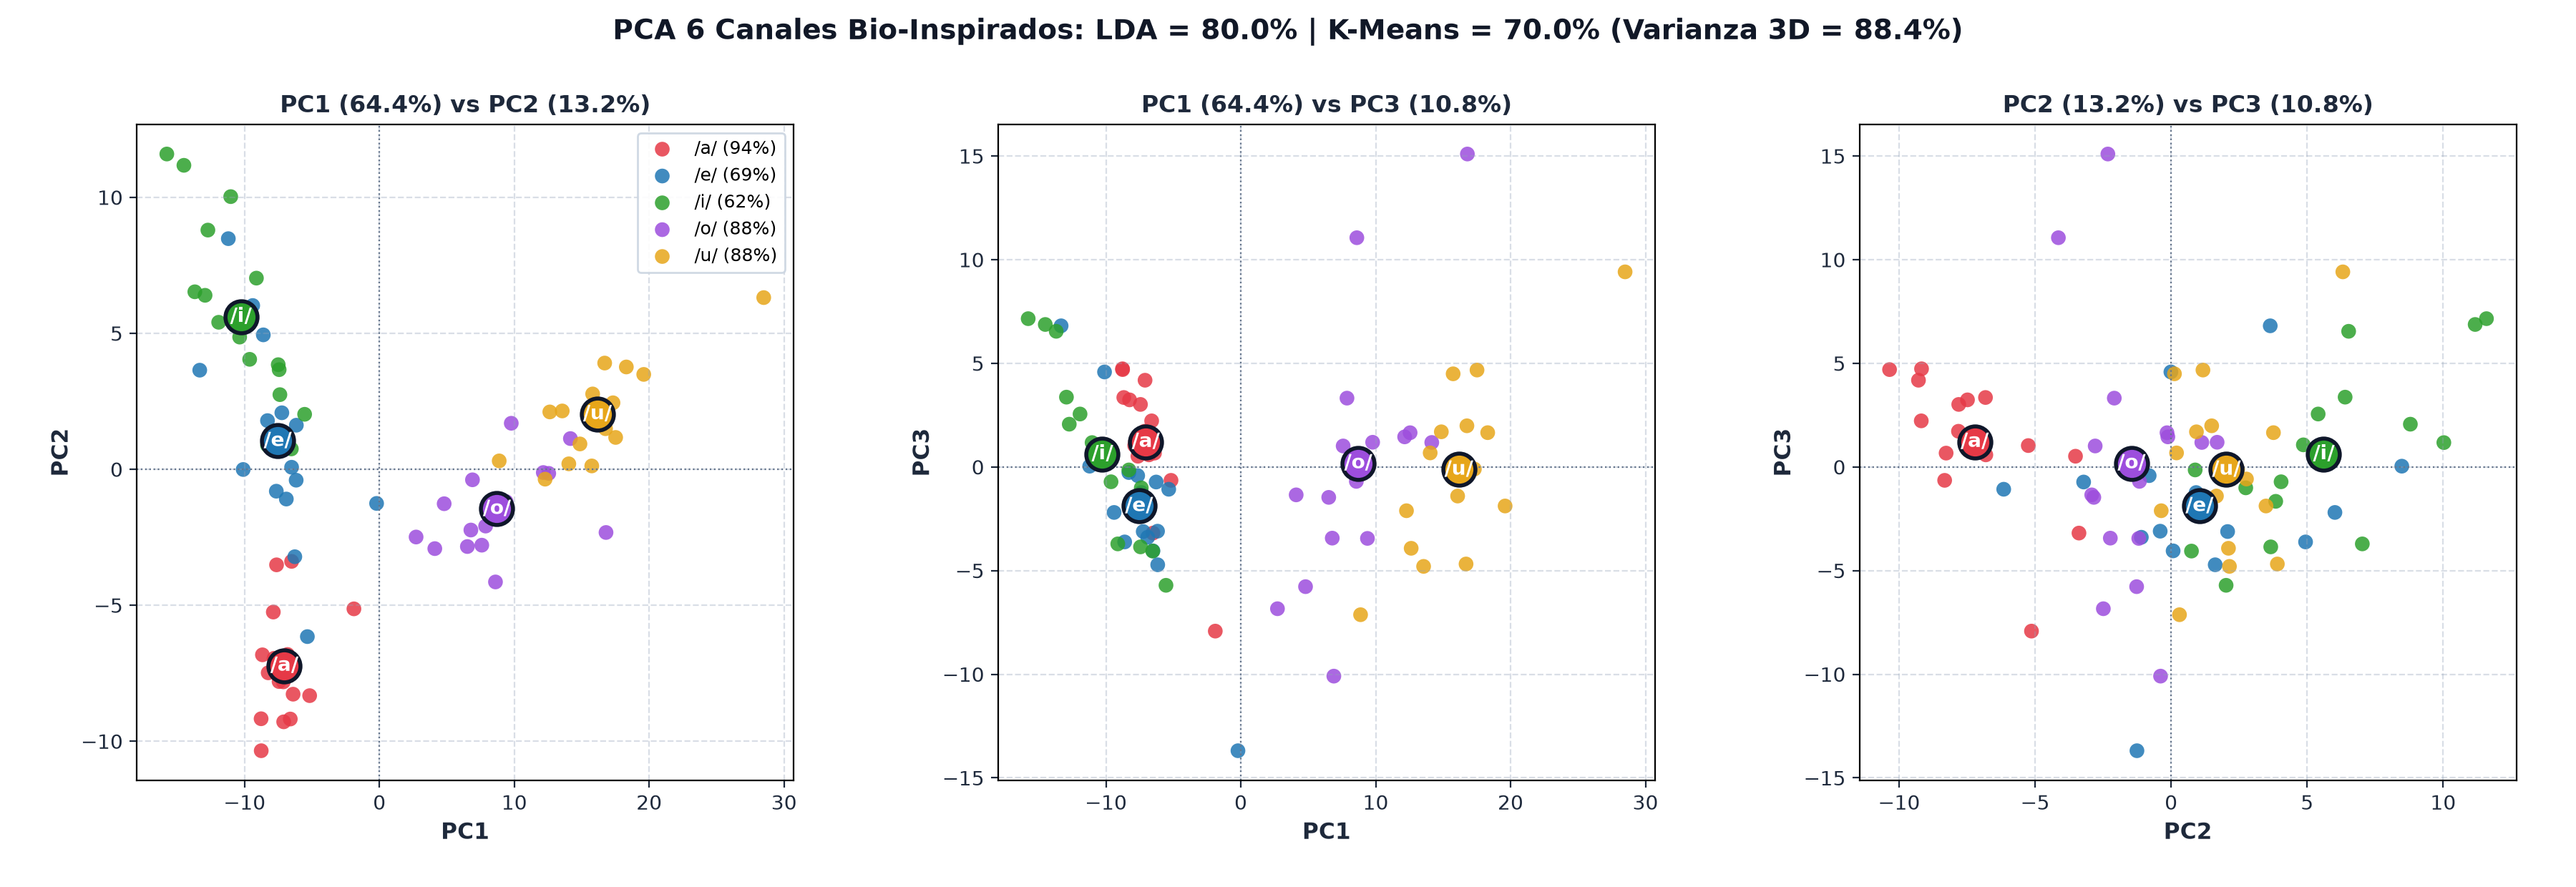
\includegraphics[width=\textwidth]{figuras/exp4/pca_6canales_oficial.png}
    \caption{Espacio PCA 3D (6 canales bio-inspirados) - Bloque 4: Invarianza a Distancia Focal y Rotación de Pose.}
    \label{fig:pca3d_6ch_exp4}
\end{figure}

\clearpage
\subsection{Variedades Geodésicas No Lineales: Isomap 2D}
Para evaluar la estructura no lineal intrínseca del manifold articular facial, se computaron las variedades Isomap en 2D con parámetro de conectividad óptimo $k=18$. En cada panel se contrasta lado a lado la proyección obtenida a partir de los 3 canales directos frente a la obtenida con los 6 canales bio-inspirados, incluyendo la métrica de decodificación lineal LDA en 2D.

\begin{figure}[htbp]
    \centering
    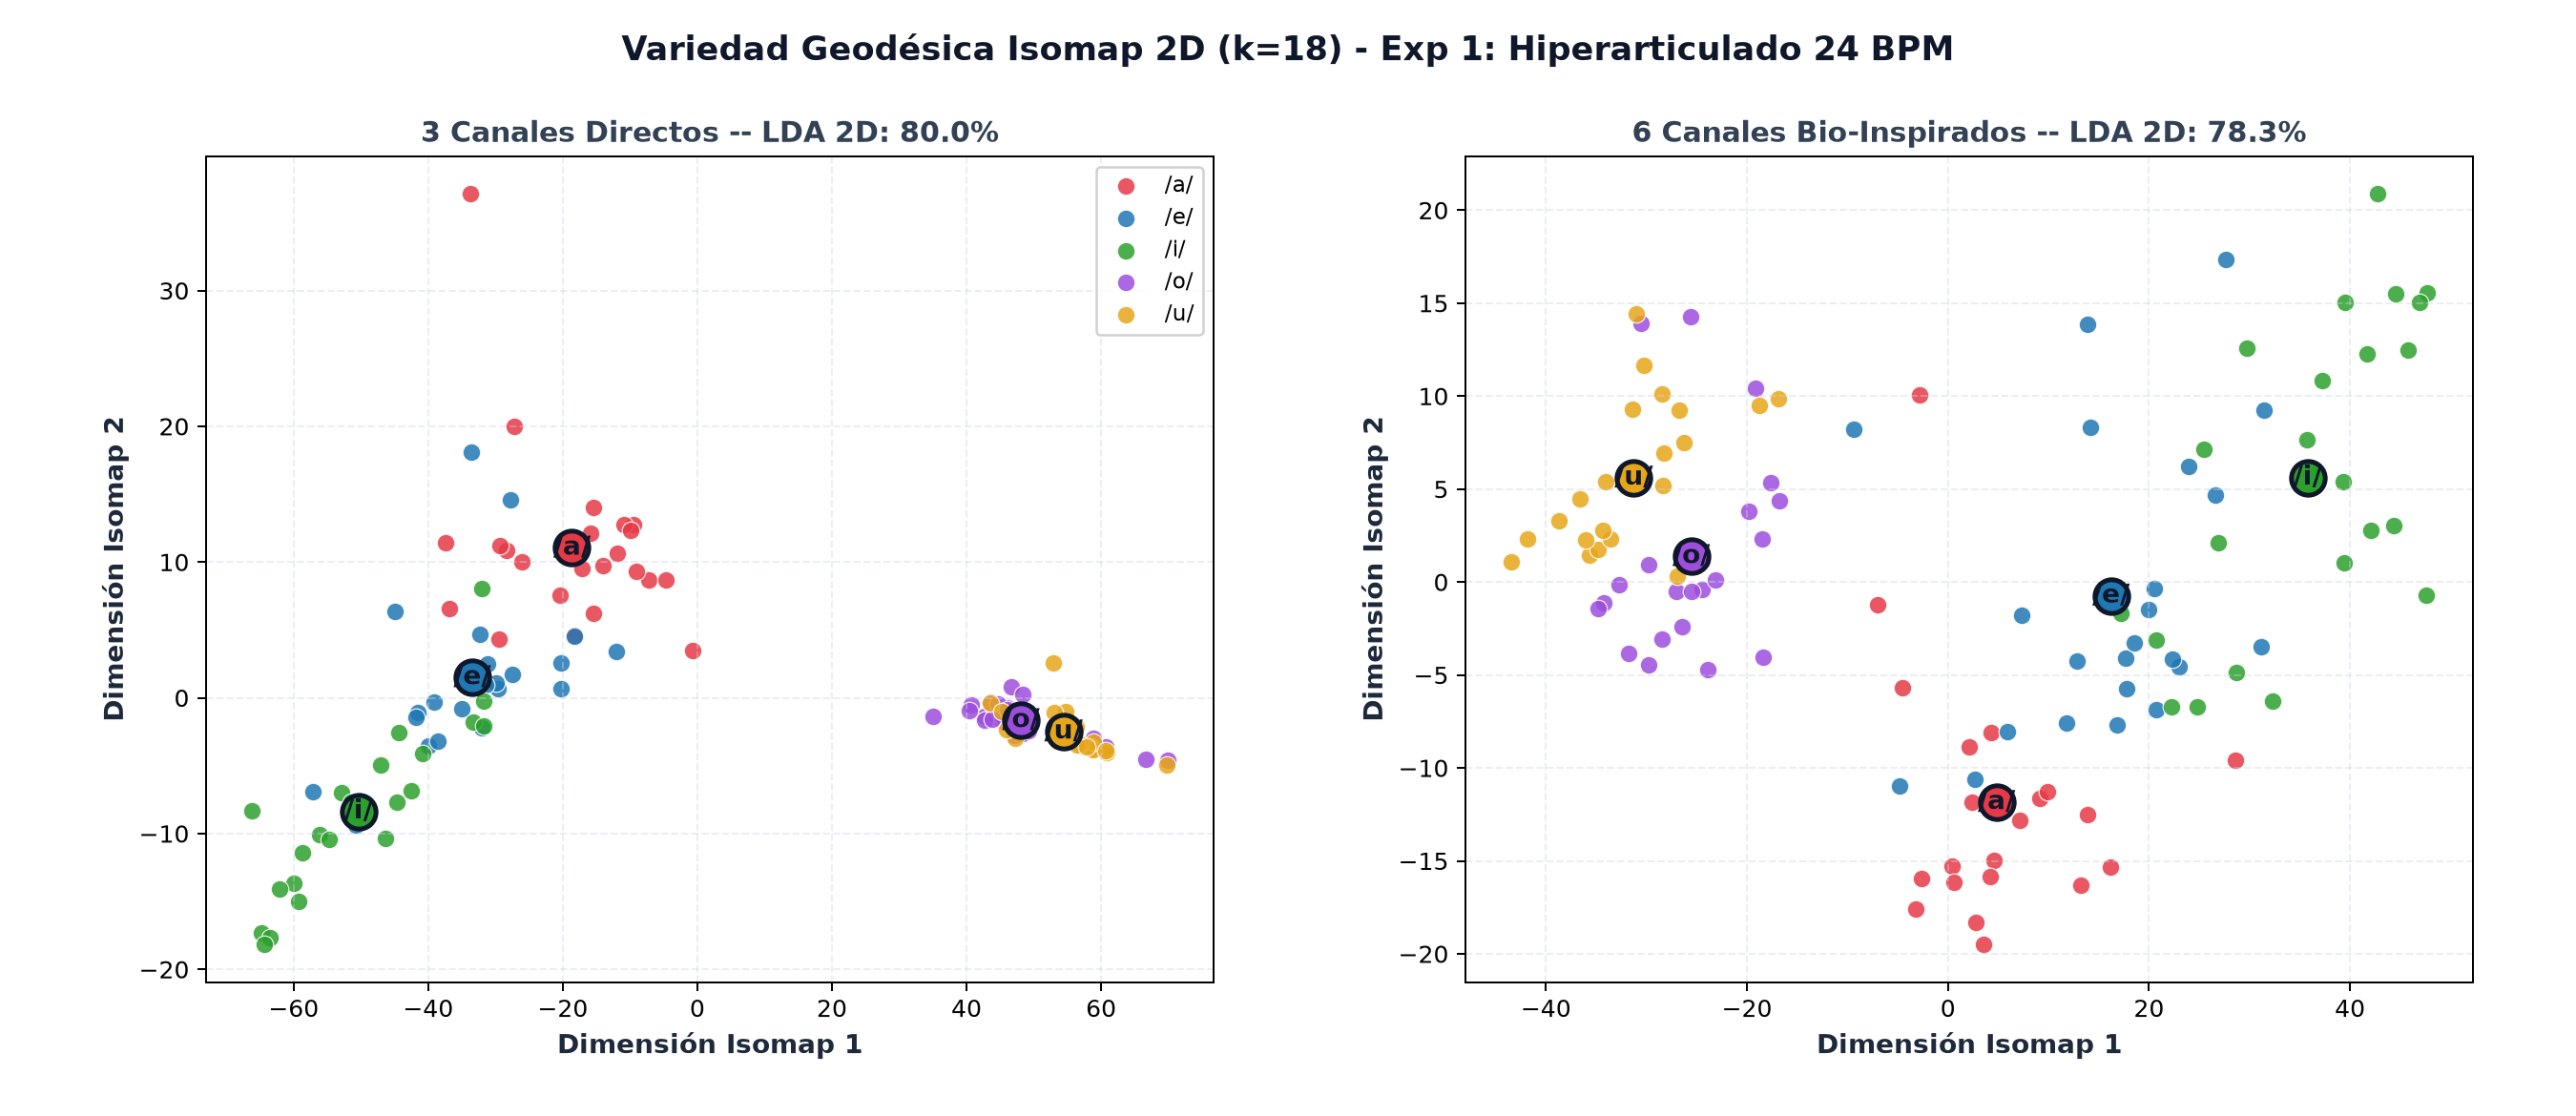
\includegraphics[width=0.95\textwidth]{figuras/exp1/isomap_2d_comparativa.png}
    \caption{Variedad Geodésica Isomap 2D ($k=18$) comparativa 3 canales vs 6 canales - Bloque 1: Hiperarticulado 24 BPM.}
    \label{fig:isomap2d_exp1}
\end{figure}

\begin{figure}[htbp]
    \centering
    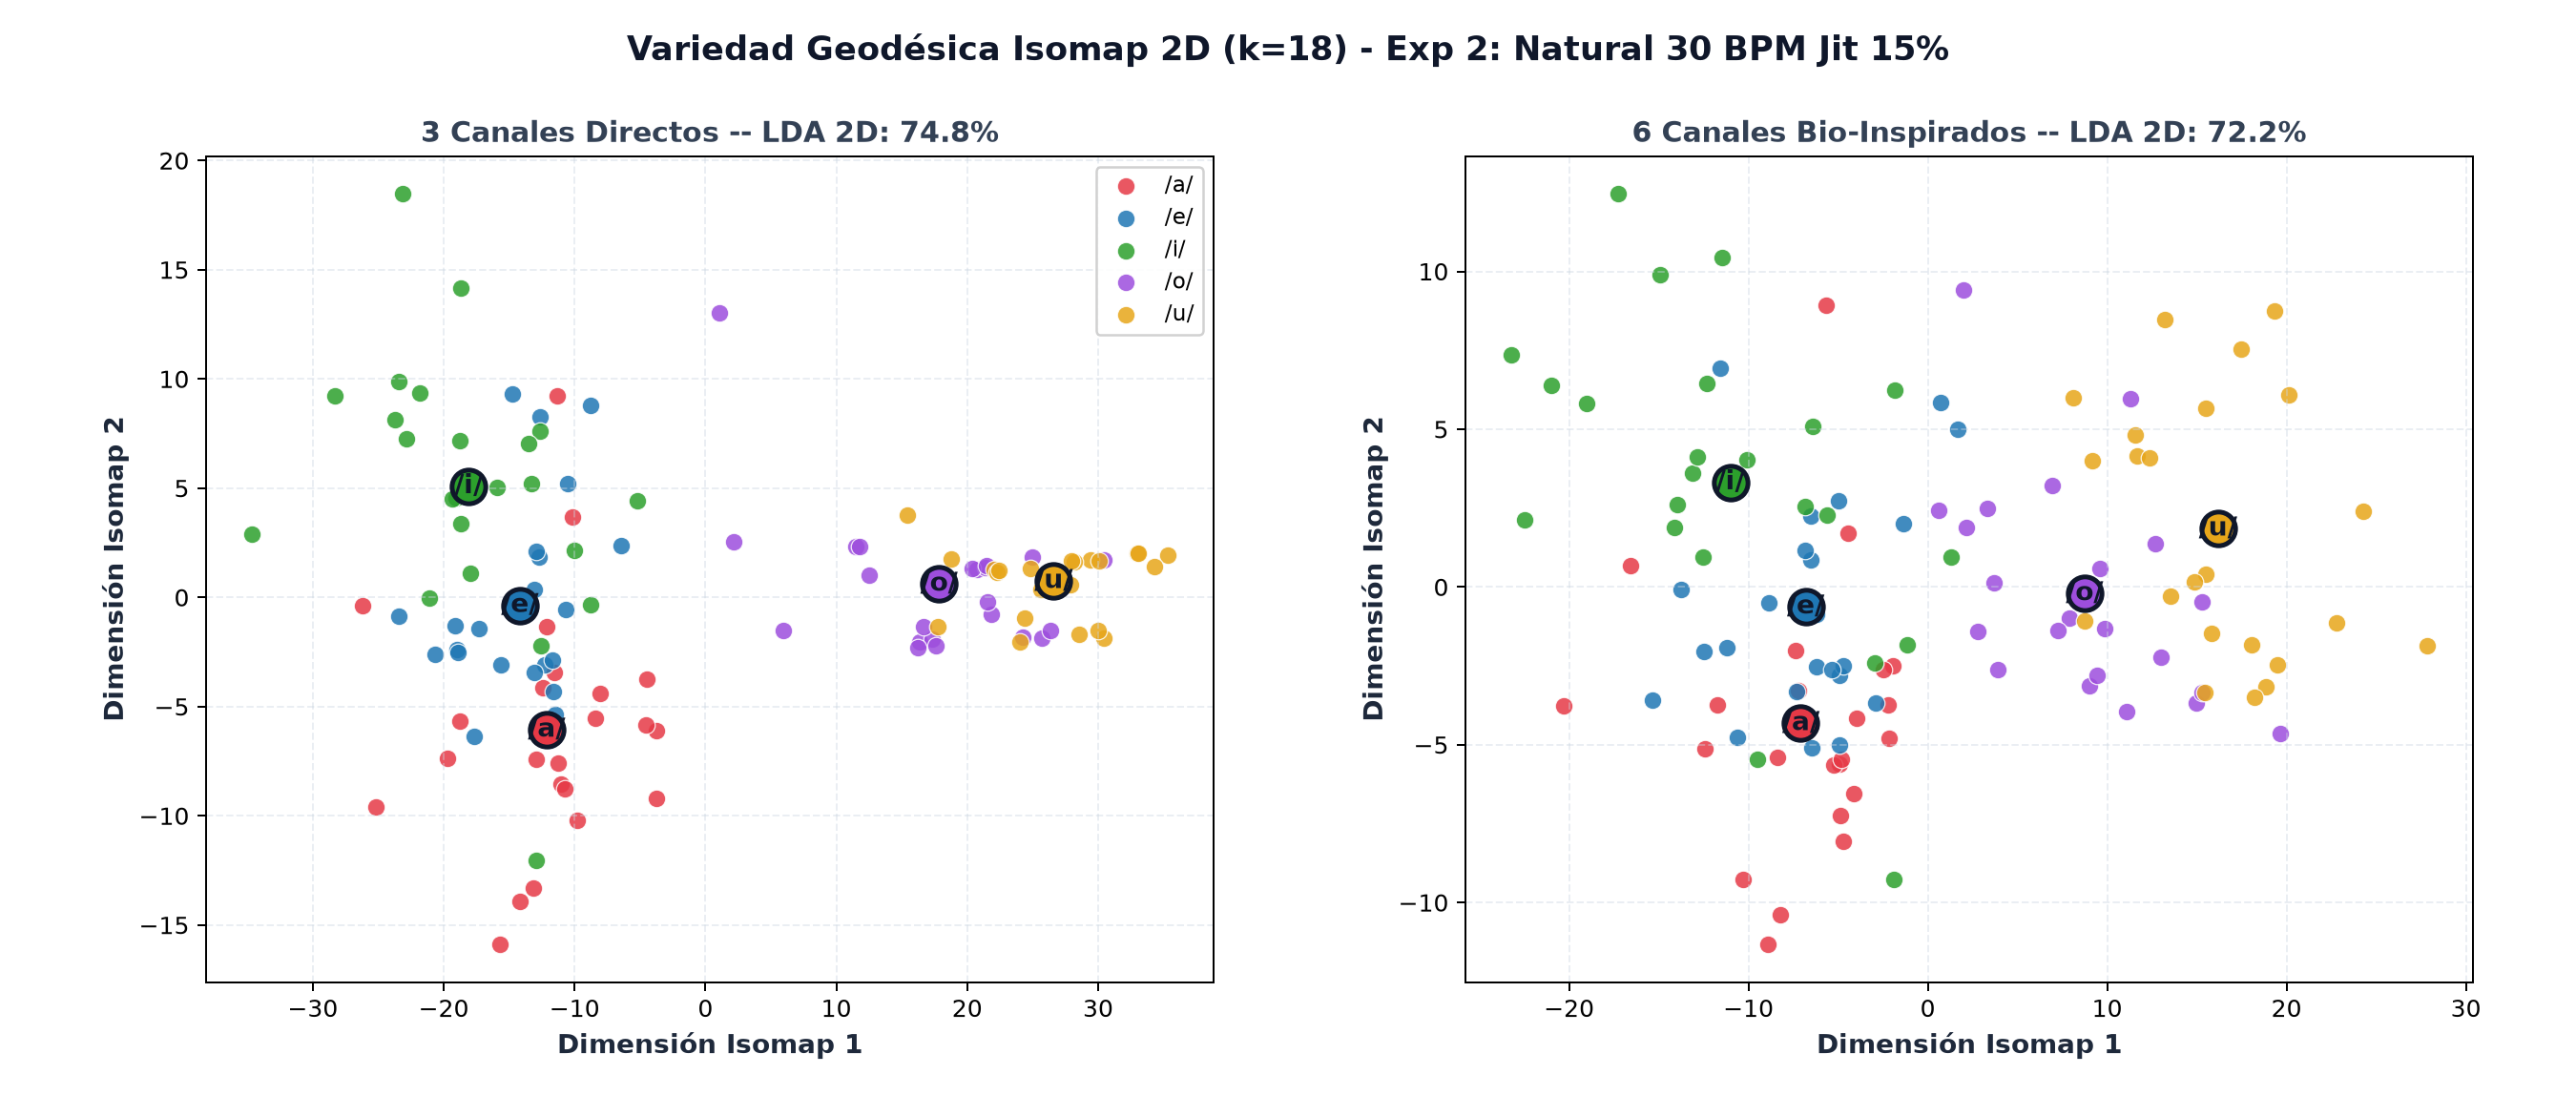
\includegraphics[width=0.95\textwidth]{figuras/exp2/isomap_2d_comparativa.png}
    \caption{Variedad Geodésica Isomap 2D ($k=18$) comparativa 3 canales vs 6 canales - Bloque 2: Cadencia Natural 30 BPM Jitter 15\%.}
    \label{fig:isomap2d_exp2}
\end{figure}

\begin{figure}[htbp]
    \centering
    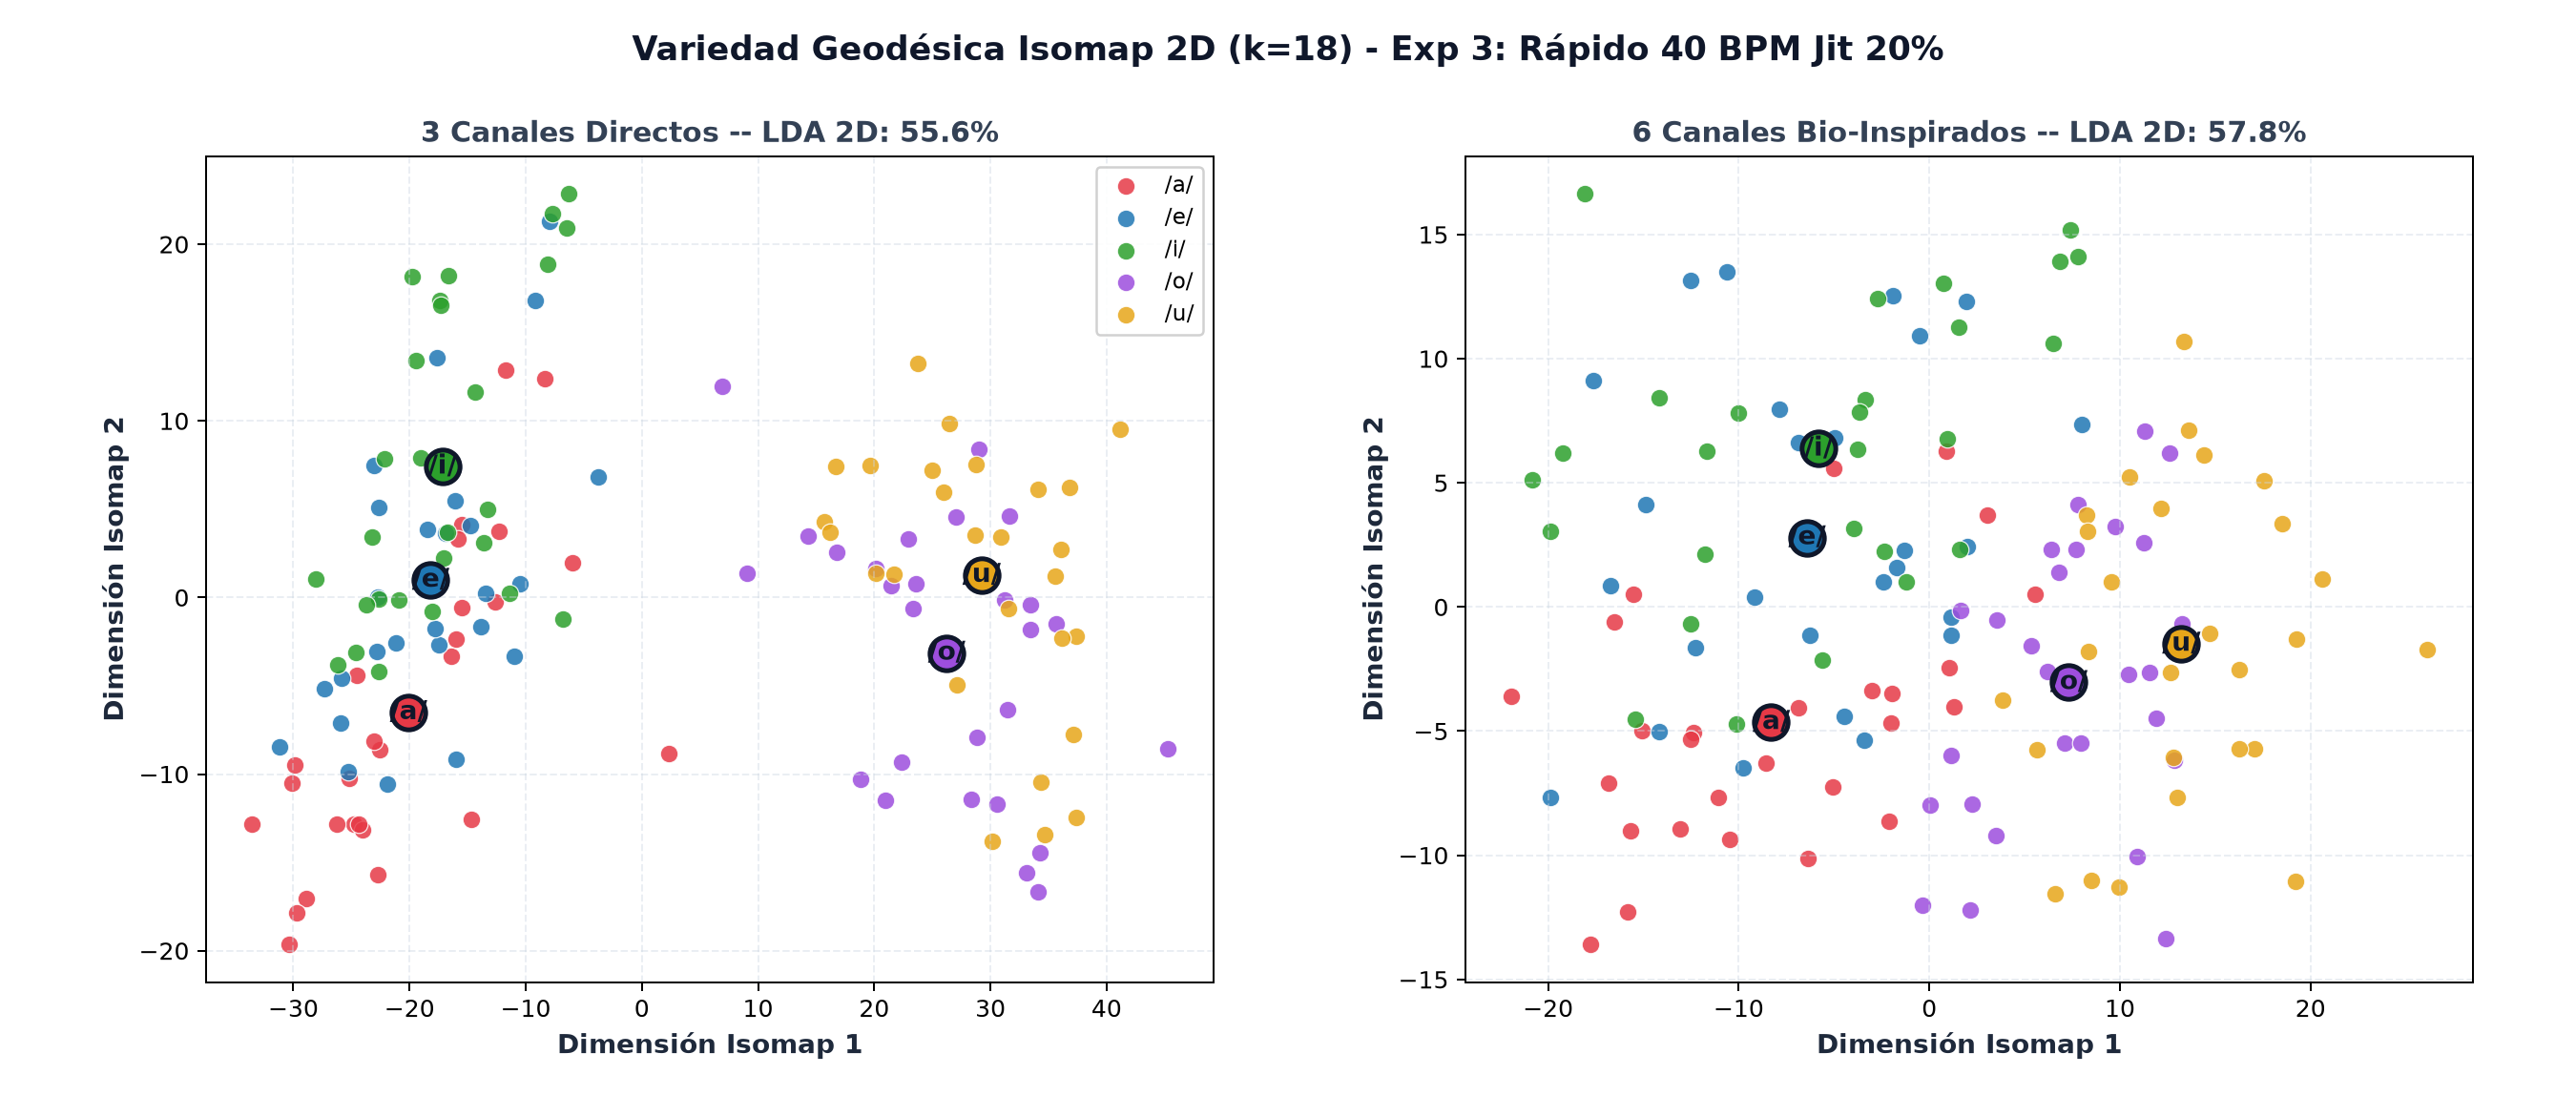
\includegraphics[width=0.95\textwidth]{figuras/exp3/isomap_2d_comparativa.png}
    \caption{Variedad Geodésica Isomap 2D ($k=18$) comparativa 3 canales vs 6 canales - Bloque 3: Cadencia Rápida 40 BPM Jitter 20\%.}
    \label{fig:isomap2d_exp3}
\end{figure}

\begin{figure}[htbp]
    \centering
    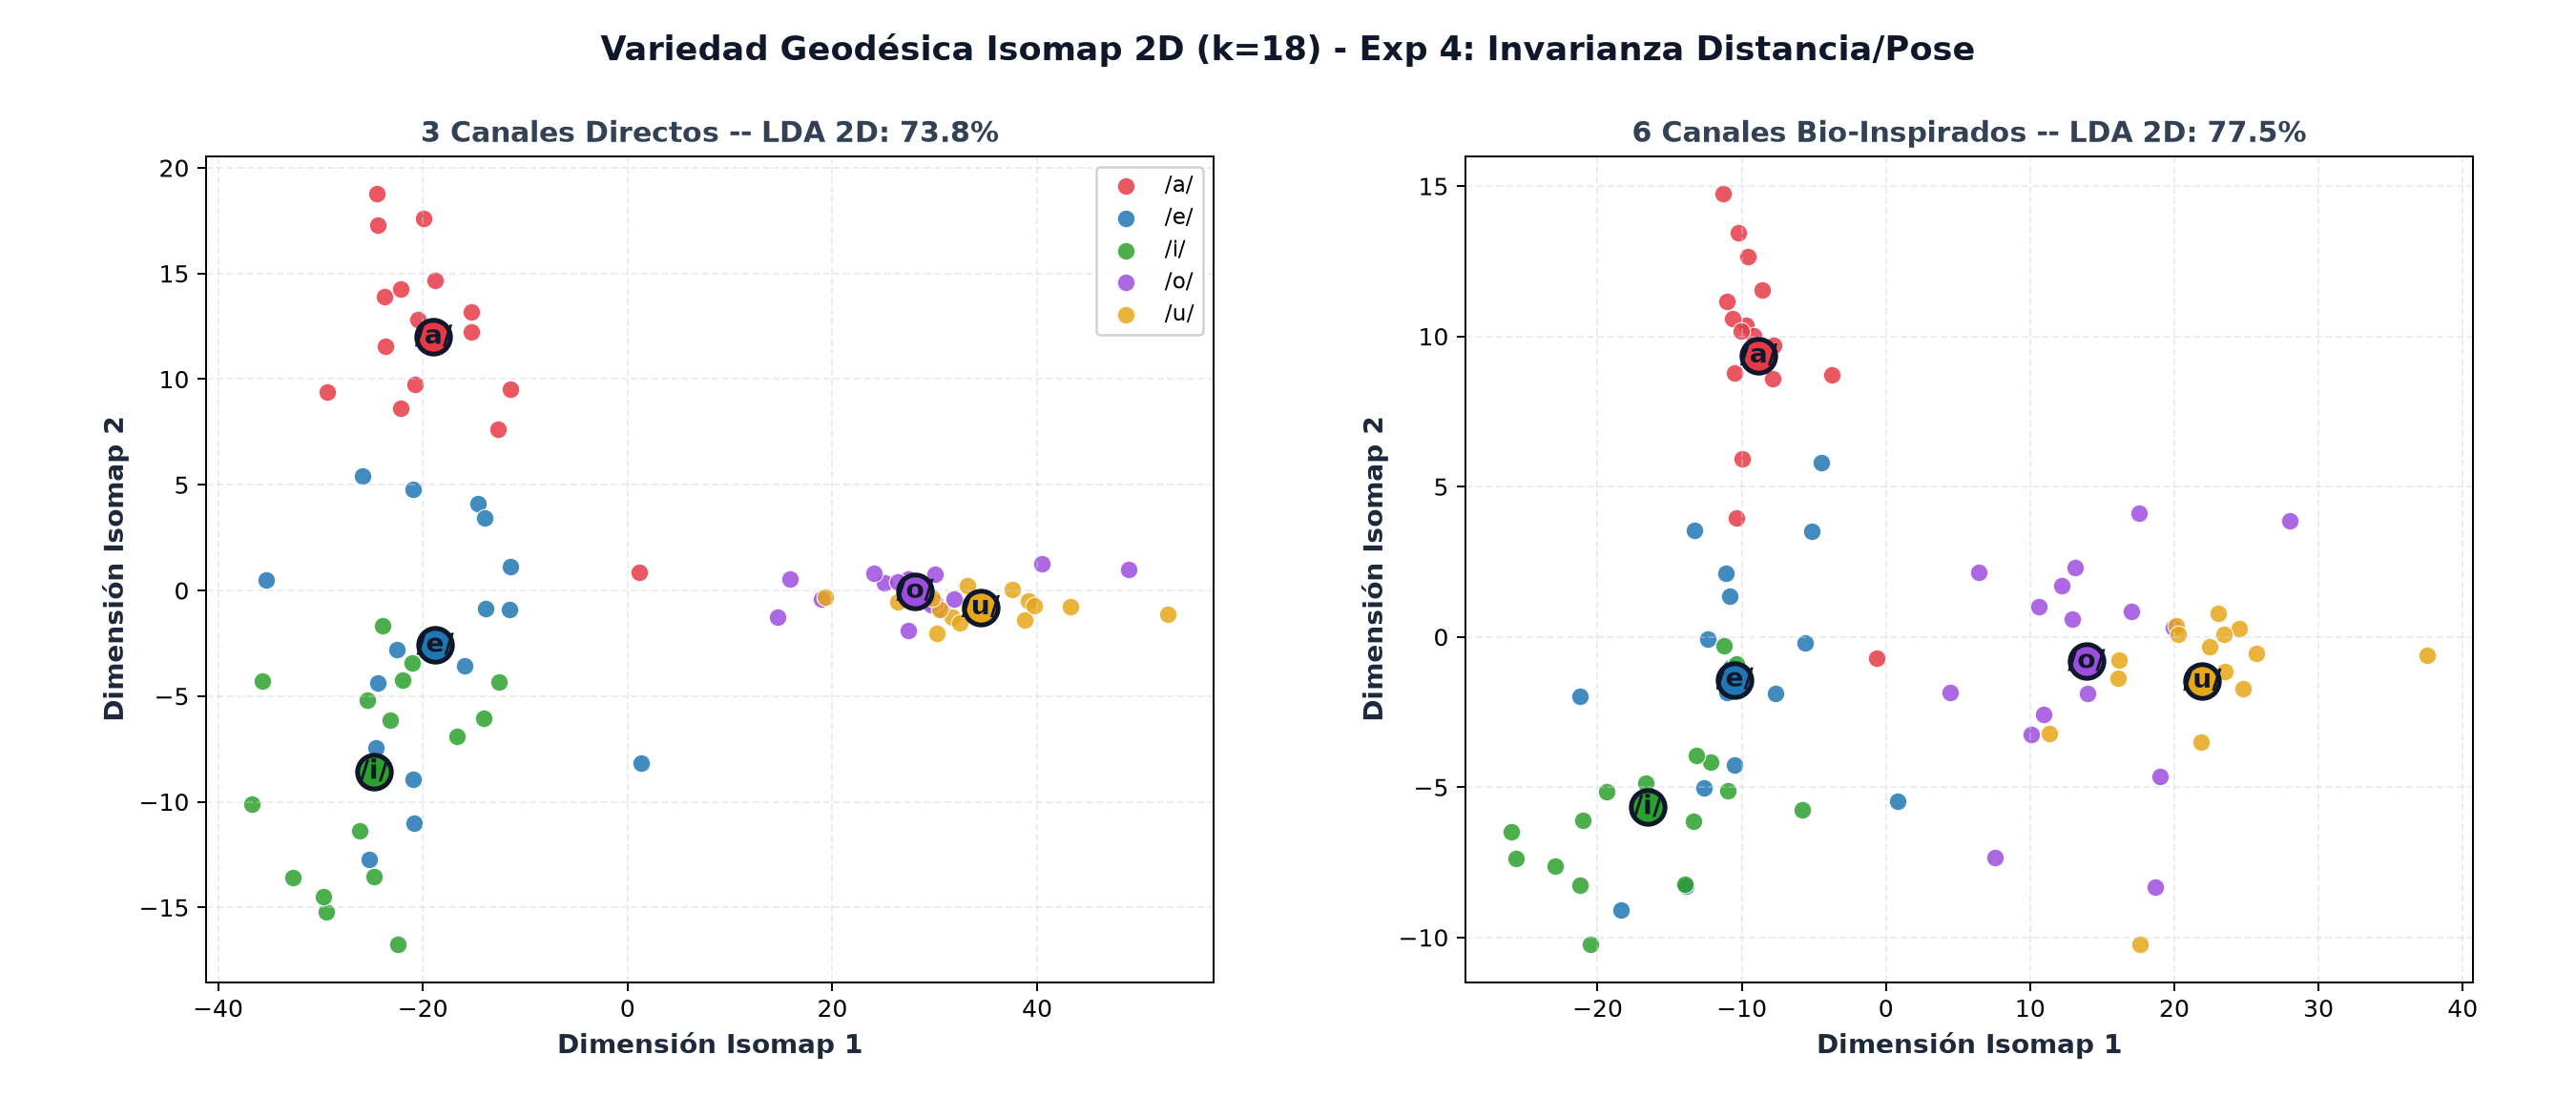
\includegraphics[width=0.95\textwidth]{figuras/exp4/isomap_2d_comparativa.png}
    \caption{Variedad Geodésica Isomap 2D ($k=18$) comparativa 3 canales vs 6 canales - Bloque 4: Invarianza a Distancia Focal y Rotación de Pose.}
    \label{fig:isomap2d_exp4}
\end{figure}

\subsection{Hallazgos Principales}
\begin{enumerate}
    \item \textbf{Efecto de Hipo-Articulación Mandibular por Cadencia:} A 24 BPM, la apertura mandibular en /a/ alcanza picos superiores a los $18.5\,\text{mm}$ con una precisión de clasificación de $81.7\%$. A 40 BPM, el hablante contrae el rango articular externo a un tercio, compensando fonéticamente con la cavidad oral interna y el cuerpo lingual, lo que reduce la separabilidad lineal puramente óptica a $65.9\%$.
    \item \textbf{Robustez del Marco Fiduciario Ortogonal:} El Bloque 4 confirma que las perturbaciones intencionales de distancia focal y rotación cefálica no degradan el clasificador cinemático, manteniendo una exactitud de $80.0\%$, idéntica a la condición hiperarticulada estática.
    \item \textbf{Complementariedad con sEMG:} La cinemática óptica provee una observación precisa de la deformación superficial del labio y mentón, sirviendo como fuente multimodal idónea para complementar las señales mioeléctricas profundas en el decodificador fonético continuo.
\end{enumerate}

\end{document}
